%%%%%%%%%%%%%%%%%%%%%%%%%%%%%%%%%%%%%%%%%%%%%%%%%%%%
% Document type, global settings, and packages
%%%%%%%%%%%%%%%%%%%%%%%%%%%%%%%%%%%%%%%%%%%%%%%%%%%%

\documentclass[12pt]{report}   %12 point font for Times New Roman
\usepackage{graphicx}  %for images and plots
\usepackage[letterpaper, left=1.5in, right=1in, top=1in, bottom=1in]{geometry}
\usepackage[doublespacing]{setspace}  %use this package to set linespacing as desired
\usepackage{times}  %set Times New Roman as the font
\usepackage[explicit]{titlesec}  %title control and formatting
\usepackage[titles]{tocloft}  %table of contents control and formatting
\usepackage[backend=bibtex, sorting=none]{biblatex}  %reference manager
\usepackage[bookmarks=true, hidelinks]{hyperref}
\usepackage[page]{appendix}  %for appendices
\usepackage{rotating}  %for rotated, landscape images

% added later below
\usepackage{tabularx}
\usepackage{amsmath}
\usepackage{subfigure}
\usepackage{multirow}
\usepackage{booktabs}
\usepackage{amssymb}
\usepackage{graphicx}
\usepackage{enumitem}
\usepackage{url}
\usepackage{xcolor}

%%%%%%%%%%%%%%%%%%%%%%%%%%%%%%%%%%%
% Bibliography
%%%%%%%%%%%%%%%%%%%%%%%%%%%%%%%%%%%

%Add your bibliography file here
\bibliography{refs}
% prevent certain fields in references from printing in bibliography
\AtEveryBibitem{\clearfield{issn}}
\AtEveryBibitem{\clearlist{issn}}

\AtEveryBibitem{\clearfield{language}}
\AtEveryBibitem{\clearlist{language}}

\AtEveryBibitem{\clearfield{doi}}
\AtEveryBibitem{\clearlist{doi}}

\AtEveryBibitem{\clearfield{url}}
\AtEveryBibitem{\clearlist{url}}

\AtEveryBibitem{%
  \ifentrytype{online}
    {}
    {\clearfield{urlyear}\clearfield{urlmonth}\clearfield{urlday}}}

%%%%%%%%%%%%%%%%%%%%%%
% Start of Document
%%%%%%%%%%%%%%%%%%%%%%

\begin{document}
%\doublespacing  %set line spacing

%%%%%%%%%%%%%%%%%%%%%%%%%%%%%%%%%%%%%
% Title Page
%%%%%%%%%%%%%%%%%%%%%%%%%%%%%%%%%%%%%
\currentpdfbookmark{Title Page}{titlePage}  %add PDF bookmark for this page
%% Define your thesis title, your name, your school, and your month and year of graduation here
\newcommand{\thesisTitle}{Data-driven pitch correction for singing}

\newcommand{\yourName}{Sanna Catherine de Treville Wager}
\newcommand{\yourDepartment}{Luddy School of Informatics, Computing, and Engineering}
\newcommand{\yourSchool}{Indiana University Bloomington}
\newcommand{\yourMonth}{February}
\newcommand{\yourYear}{2021}

%%%%%%%%%%%%%%%%%%%%%%%%%%%%%%%%%%%%%%%%%%%%%%%%%%%%%%%%%
% Do not edit these lines unless you wish to customize
% the template
%%%%%%%%%%%%%%%%%%%%%%%%%%%%%%%%%%%%%%%%%%%%%%%%%%%%%%%%%



\begin{titlepage}
\newgeometry{top=2in}
\begin{center}

{\large \MakeUppercase{\thesisTitle}}\\
\vspace{7\baselineskip}
\yourName\\
\vfill
Submitted to the faculty of the University Graduate School\\
in partial fulfillment of the requirements\\
for the degree\\
Doctor of Philosophy\\
in the Department of \yourDepartment,\\
\yourSchool\\
\yourMonth{} \yourYear{}

\end{center}
\restoregeometry
\end{titlepage}


%%%%%%%%%%%%%%%%%%%%%%%%%%%%%%%%%%%%%
% Approval Page
%%%%%%%%%%%%%%%%%%%%%%%%%%%%%%%%%%%%%
\pagenumbering{roman}
\setcounter{page}{2} % set the page number appropriately based on the number of intro pages
\newpage
%% Define your committee members. If you have less than 6, simple delete/comment the unused lines

\newcommand{\committeeChairpersonTypedName}{Minje Kim}
\newcommand{\committeeChairpersonPostNominalInitials}{Ph.D.}

\newcommand{\committeeMemberTwoTypedName}{Daniel J. McDonald}
\newcommand{\committeeMemberTwoPostNominalInitials}{Ph.D.}

\newcommand{\committeeMemberThreeTypedName}{Christopher Raphael}
\newcommand{\committeeMemberThreePostNominalInitials}{Ph.D.}

\newcommand{\committeeMemberFourTypedName}{Donald S. Williamson}
\newcommand{\committeeMemberFourPostNominalInitials}{Ph.D.}

% Uncomment to add another committee member
%\newcommand{\committeeMemberFiveTypedName}{Name}
%\newcommand{\committeeMemberFivePostNominalInitials}{Post-Nominal Initials}

\newcommand{\myRule}{\rule{0.5\textwidth}{0.4pt}}

\newcommand{\approvalDay}{10}
\newcommand{\approvalMonth}{01}
\newcommand{\approvalYear}{2020}

%%%%%%%%%%%%%%%%%%%%%%%%%%%%%%%%%%%%%%%%%%%%%%%%%%%%%%%%%
% Do not edit these lines unless you wish to customize
% the template
%%%%%%%%%%%%%%%%%%%%%%%%%%%%%%%%%%%%%%%%%%%%%%%%%%%%%%%%%


\newgeometry{left=1in}

\begin{center}
 
Accepted by the Graduate Faculty, Indiana University, in partial fulfillment of the requirements for the degree of Doctor of Philosophy.

\end{center}

\vspace{2\baselineskip}

\ifdefined\committeeMemberFourTypedName
Doctoral Committee\\

\null\hfill \myRule\\
\null\hfill \committeeChairpersonTypedName, \committeeChairpersonPostNominalInitials\\
\null\hfill \myRule\\
\null\hfill \committeeMemberTwoTypedName, \committeeMemberTwoPostNominalInitials\\
\null\hfill \myRule\\
\null\hfill \committeeMemberThreeTypedName, \committeeMemberThreePostNominalInitials\\
\null\hfill \myRule\\
\null\hfill \committeeMemberFourTypedName, \committeeMemberFourPostNominalInitials\\

\ifdefined\committeeMemberFiveTypedName
\null\hfill \myRule\\
\null\hfill \committeeMemberFiveTypedName, \committeeMemberFivePostNominalInitials\\
\fi

\fi
\vfill
Date of Defense: \approvalMonth/\approvalDay/\approvalYear
\restoregeometry


%%%%%%%%%%%%%%%%%%%%%%%%%%%%%%%%%%%%%
% Copyright
%%%%%%%%%%%%%%%%%%%%%%%%%%%%%%%%%%%%%
\newpage
%%%%%%%%%%%%%%%%%%%%%%%%%%%%%%%%%%%%%%%%%%%%%%%%%%%%%%%%%
% Do not edit these lines unless you wish to customize
% the template
%%%%%%%%%%%%%%%%%%%%%%%%%%%%%%%%%%%%%%%%%%%%%%%%%%%%%%%%%

\clearpage
\begin{center}

\vspace*{\fill}
Copyright \copyright{} \yourYear{}\\
\yourName
\vspace*{\fill}

\end{center}
\clearpage


%%%%%%%%%%%%%%%%%%%%%%%%%%%%%%%%%%%%%
% Dedication
%%%%%%%%%%%%%%%%%%%%%%%%%%%%%%%%%%%%%
\newpage
% Define your dedication statement here

\newcommand{\yourDedication}{To my family.}

%%%%%%%%%%%%%%%%%%%%%%%%%%%%%%%%%%%%%%%%%%%%%%%%%%%%%%%%%
% Do not edit these lines unless you wish to customize
% the template
%%%%%%%%%%%%%%%%%%%%%%%%%%%%%%%%%%%%%%%%%%%%%%%%%%%%%%%%%

\begin{center}

\vspace*{\fill}
\yourDedication\\
%Multiple design decisions lie behind any sound that reaches our ears. Given the current design of processors, contDesign starts with the way a continuous, acoustic signal is represented as a discrete sequence of  is built on multiple design decision, ranging from the 
%We interact with digital music on a regular basis, through music recordings and streaming, electric instruments, and tools such as microphones and recording devices.  


%Through college, my music making was first and foremost in the acoustic realm. I was trained in the Western Classical tradition, first on piano, then on bassoon. Even then, I interacted with digital music on a daily basis, through the radio, music streaming apps, electric keyboards, and tools such as microphones, tuners, and recording devices. In college, I grew curious about the representations of music as data in the digital realm. I became aware of how behind all of them were design decisions by audio and software engineers. I wished to understand how these representations could affect our experience of music, for the better, for the worse, or some of both. Conveniently, a graduate degree existed for this, named music informatics. 

%The question arises of what place apps hold in the world of music making. Apps can easily come across as toys, too musically limiting to enable the user's lifelong pursuit of excellence that is music learning. At the 2017 Audio Developer Conference keynote,\footnote{``Julian Storer - Keynote: Does your code actually matter? (ADC’17).'' YouTube Video, 0:00. Posted November 17, 2017. https://youtu.be/Yd0Ef6uzJb0} Julian Storer described how even engineers working on digital audio processing tools for professional musicians sometimes wondered whether they were building gadgets.\footnote{Thank you to Google and my intern host, Glenn Kasten, for funding my trip to the Audio Developer Conference.}

%During my internship with Smule, Inc.---a singing app---in 2018, I learned how some users will take a ten-minute break in their car in the middle of a workday to sing. Many have written to the company to thank it for bringing them joy and relief from stress. For some people, these ten-minute breaks are all the music that they have the time to make on a regular basis. This is one example of how apps have the potential to play a significant role in one's musical experience, and that with high-quality technology these experiences can be musically rich. Having personally started singing during graduate school, I found that Smule provided a good framework for learning songs, and was inspired by the experience. For some, an app can serve as an entryway into music. Especially in the case of people who do not grow up with much exposure to music, or do not have acoustic musical instruments easily available, digital audio and apps might be the main way to interact with music. The quality of the sound and musical richness in these apps might even influence whether a person develops a deeper interest in music making or gives it up. 

\vspace*{\fill}

\end{center}

%%%%%%%%%%%%%%%%%%%%%%%%%%%%%%%%%%%%%
% Acknowledgments
%%%%%%%%%%%%%%%%%%%%%%%%%%%%%%%%%%%%%
\newpage
\phantomsection
\addcontentsline{toc}{chapter}{Acknowledgements}
\begin{centering}
\textbf{ACKNOWLEDGEMENTS}\\
\vspace{\baselineskip}
\end{centering}

%Insert your dedication text here
Lorem ipsum dolor sit amet, consectetur adipiscing elit, sed do eiusmod tempor incididunt ut labore et dolore magna aliqua. Ut enim ad minim veniam, quis nostrud exercitation ullamco laboris nisi ut aliquip ex ea commodo consequat. Duis aute irure dolor in reprehenderit in voluptate velit esse cillum dolore eu fugiat nulla pariatur. Excepteur sint occaecat cupidatat non proident, sunt in culpa qui officia deserunt mollit anim id est laborum.



%%%%%%%%%%%%%%%%%%%%%%%%%%%%%%%%%%%%%
% Abstract
%%%%%%%%%%%%%%%%%%%%%%%%%%%%%%%%%%%%%
\newpage
\phantomsection
\addcontentsline{toc}{chapter}{Abstract}
%%%%%%%%%%%%%%%%%%%%%%%%%%%%%%%%%%%%%%%%%%%%%%%%%%%%%%%%%
% Do not edit these lines unless you wish to customize
% the template
%%%%%%%%%%%%%%%%%%%%%%%%%%%%%%%%%%%%%%%%%%%%%%%%%%%%%%%%%
\newgeometry{left=1in}

\begin{center}

\yourName\\
\MakeUppercase{\thesisTitle}

\end{center}

\vspace{1.5\baselineskip}

%Insert your abstract here



In this thesis, I introduce a data-driven algorithm for pitch correction of monophonic singing performances. The algorithm uses reference pitches in the accompaniment track to predict shifts in the vocals track. It involves a deep neural network model that learns musical intonation patterns from 4,702 amateur karaoke performances selected for accuracy. The model is exposed both to incorrect intonation, for which it learns a correction, and intentional pitch variation, which it learns to preserve. The proposed algorithm represents pitch as a continuous value, differing from existing commercial systems, where vocal track notes are usually mapped to one of the twelve equal-tempered scale degrees. In this thesis, I argue---based on evidence from musical studies and from theoretical writings on musical intonation---that few musical traditions fit the equal-tempered scale. Deviations from the scale are often a crucial musical component, and the model can be trained on music from a given culture to preserve its deviations. I argue further in favor of a data-driven approach to digital music processing over a model-based approach, prioritizing expressivity over control and interpretability. The proposed deep neural network with gated recurrent units on top of convolutional layers shows promising performance on the real-world score-free singing pitch correction task. 



\ifdefined\committeeMemberFourTypedName

\null\hfill \myRule\\
\null\hfill \committeeChairpersonTypedName, \committeeChairpersonPostNominalInitials\\
\null\hfill \myRule\\
\null\hfill \committeeMemberTwoTypedName, \committeeMemberTwoPostNominalInitials\\
\null\hfill \myRule\\
\null\hfill \committeeMemberThreeTypedName, \committeeMemberThreePostNominalInitials\\
\null\hfill \myRule\\
\null\hfill \committeeMemberFourTypedName, \committeeMemberFourPostNominalInitials\\

\ifdefined\committeeMemberFiveTypedName
\null\hfill \myRule\\
\null\hfill \committeeMemberFiveTypedName, \committeeMemberFivePostNominalInitials\\
\fi

\fi
\restoregeometry



%%%%%%%%%%%%%%%%%%%%%%%%%%%%%%%%%%%%%
% Table of Contents
%%%%%%%%%%%%%%%%%%%%%%%%%%%%%%%%%%%%%

% Format for Table of Contents
\renewcommand{\cftchapdotsep}{\cftdotsep}  %add dot separators
\renewcommand{\cftchapfont}{\bfseries}  %set title font weight
\renewcommand{\cftchappagefont}{}  %set page number font weight
\renewcommand{\cftchappresnum}{Chapter }
\renewcommand{\cftchapaftersnum}{:}
\renewcommand{\cftchapnumwidth}{5em}
\renewcommand{\cftchapafterpnum}{\vskip\baselineskip} %set correct spacing for entries in single space environment
\renewcommand{\cftsecafterpnum}{\vskip\baselineskip}  %set correct spacing for entries in single space environment
\renewcommand{\cftsubsecafterpnum}{\vskip\baselineskip} %set correct spacing for entries in single space environment
\renewcommand{\cftsubsubsecafterpnum}{\vskip\baselineskip} %set correct spacing for entries in single space environment

%format title font size and position (this also applys to list of figures and list of tables)
\titleformat{\chapter}[display]
{\normalfont\bfseries\filcenter}{\chaptertitlename\ \thechapter}{0pt}{\MakeUppercase{#1}}

\renewcommand\contentsname{Table of Contents}
\currentpdfbookmark{Table of Contents}{TOC}
\begin{singlespace}
\tableofcontents
\end{singlespace}


\clearpage

%%%%%%%%%%%%%%%%%%%%%%%%%%%%%%%%%%%%%
% List of figures and tables
%%%%%%%%%%%%%%%%%%%%%%%%%%%%%%%%%%%%%
\phantomsection
\addcontentsline{toc}{chapter}{List of Tables}
\begin{singlespace}
\setlength\cftbeforetabskip{\baselineskip}  %manually set spacing between entries
\listoftables
\end{singlespace}

\clearpage

\phantomsection
\addcontentsline{toc}{chapter}{List of Figures}
\begin{singlespace}
\setlength\cftbeforefigskip{\baselineskip}  %manually set spacing between entries
\listoffigures
\end{singlespace}

\clearpage

%%%%%%%%%%%%%%%%%%%%%%%%%%%%
%
% Chapters
%
%%%%%%%%%%%%%%%%%%%%%%%%%%%%

%%%%%%%%%%%%%%%%%%%%%%
% formatting
%%%%%%%%%%%%%%%%%%%%%%

% resume page numbering for rest of document
\clearpage
\pagenumbering{arabic}
\setcounter{page}{1} % set the page number appropriately

% Adjust chapter title formatting
\titleformat{\chapter}[display]
{\normalfont\bfseries\filcenter}{\MakeUppercase\chaptertitlename\ \thechapter}{0pt}{\MakeUppercase{#1}}  %spacing between titles
\titlespacing*{\chapter}
  {0pt}{0pt}{30pt}	%controls vertical margins on title
  
% Adjust section title formatting
\titleformat{\section}{\normalfont\bfseries}{\thesection}{1em}{#1}

% Adjust subsection title formatting
\titleformat{\subsection}{\normalfont\bfseries}{\thesubsection}{1em}{#1}

% Adjust subsubsection title formatting
\titleformat{\subsubsection}{\normalfont\itshape}{\thesubsubsection}{1em}{#1}

%%%%%%%%%%%%%%%%
% Chapter 1
%%%%%%%%%%%%%%%%

\chapter{Introduction}
\label{chap:thesis-intro}
%\section{Post-processing of user-generated audio: An overview}
%\label{sec:challenges-intro}
%1. Introduction to the introduction. 
%    1. Deep autotuner
%        1. Automatic pitch correction system (define)
%        2. DNN
%        3. data-driven (define)
%        4. relationship between spectrograms/time-frequency transformations (define)
%        5. trained on real-world singing
%        6. can be adapted to musical genres w/o equal-tempered
%        7. no musical score: harmonize improvise
%        8. respect nuanced variations of sung pitch 
%        9. estimates amount of unintended pitch shift
Digital music builds on a rich music tradition in the acoustic realm, but also differs from it by nature. Before digital music can reach our ears, it needs to be represented as data that a computer can process. Design and engineering decisions lie behind this representation, from the sound wave itself---stored as a sequence of numbers---to musical structure, including melody, harmony, and rhythm. This thesis focuses on the question of representation of musical pitch in the digital realm, in the context of a pitch correction algorithm for singing voice. The way musical pitch is represented will affect how the notes are adjusted, and by extension the listener's musical experience. This thesis covers studies of how physical measures of pitch, such as frequency and timbre, map to what we hear through a complex psychoacoustic process influenced by our musical upbringing, and determine whether we consider a note to be ``in tune'' or not. It introduces a pitch correction algorithm design that strives to relate digital representation to the complex and rich way we experience pitch.

Music making with family, friends, and the wider community is one of the universally enjoyed activities across the world. In recent years, digital options have emerged in applications such as Smule, Spotify, Cadenza, YouTube, and TikTok. These enable people to share their recordings with their peers in other locations, and provide tools for collaboration and audio processing that are only possible in the digital realm. One category of tools is post-processing, which involves editing the track after it has been recorded to make it the best possible quality. Automatic pitch correction to make a performance sound in tune falls into this category. 

Why not just leave the recording unaltered? As anyone who has tried to photograph a beautiful landscape might relate to, capturing the natural colors, beauty, and atmosphere of the scene is very challenging. Image post-processing might actually make the outcome more realistic or, alternatively, focus the viewer on aspects of the landscape that would not have stood out when present in person. In the same way, a performance heard live versus recorded can be a substantially different artistic experience, where the listener is hearing the performance through the recording and playback pipeline, outside the original acoustic setting. Post-processing of audio can enhance the listening experience. 

The process of producing a digital recording can range from professional to recreational. The professional kind involves use of professional audio-editing software, high-end microphones, and recording spaces with good acoustics, all of which require considerable time and resources. It results in a high-quality, polished result. The recreational kind often involves multipurpose recording devices such as smartphones, and typically involves less time and resources. Music apps can serve as a platform for recreational music making. Apps can provide a meaningful musical opportunity. During my internship with Smule, Inc, a singing app, I heard about users who would take a ten-minute break in their workday to sing, then would write to the company sharing how that short singing break brought them joy and reduced their stress. Recreational musicians may not wish to spend much time editing their recording, or have the resources or training to do so, but still wish use post-processing tools built into the app that apply automatic pitch correction or other effects such as reverb. These post-processing tools do not replace professional audio editing, but are recognized as improving the quality of the recording with remarkably little effort or cost. Although post-processing tools fall short of bring a recording up to a professional level, they may well make it more pleasing to a listener. A parallel can be seen when a person uses a spell-checker to improve the quality of their writing, even when writing simple text such as an email. The ability of the spell-checker to remove minor errors produces a more polished result, which can make a big difference, especially given the high stakes of sharing content in a recorded format.

Digital apps may be the primary way that many people interact actively with music, or the first approach people try when getting started with music. The quality of the experience and its potential to lead to musical growth may determine whether a user keeps making music or gives it up.

\section{Overview}
This thesis addresses the task of developing a data-driven algorithm for automatic pitch correction. Existing commercial systems usually discretize the pitch to a small number of values \cite{antares:2016}. Vocal track notes are usually shifted to be centered around pitches in a user-defined score, or mapped to the closest pitch among the twelve equal-tempered scale degrees. The resulting model of pitch does not reflect the smooth variation of pitch in continuously controlled instruments such as voice or violin, and can produce a robotic-sounding result. The proposed pitch correction system uses a deep neural network trained to predict pitch shifts based on audio patterns in real-world singing examples. Through these examples, the system is exposed to both incorrect intonation, for which it learns a correction, and intentional pitch variation, which it learns to preserve. It treats pitch as a continuous value rather than a discrete set of notes and does not rely on a musical score, thus allowing for improvisation and harmonization in the singing performance. The fact that it is not bound to a discrete set of notes also means that it can be adapted to many different musical cultures, regardless of the scales used in these cultures. 

%\section{Background}
%2. Personal background: overarching topic
%    1. Technology and music have traditionally built on each other. 
%    - Undergraduate acoustic intrument, rich sounds, 
%    - Inspired by renaissance choir music
%    - Pythagoras, ratio theory, harmony of the spheres inspired me in intonation endeavors, 
%    - Stories of choirs shifting global pitch down over time to sound in tune
%    - Magic of a violin solo in Thais Massenet that hit just the right pitches
%    - jazz, always one note off. Classical music: anxious of making a mistake that would ruin the magic. Brick in a giant building of sound, didn’t want to be the one that made it tumble over
%    - Soundgarden and imperfection
%    - Magic of pitch bending in bollywood music
%    - I also found intonation very difficult: my bassoon professor McLean described how a bad timbre can make a note sound out of tune even though the tuner measures the correct frequency
%    - Bassoonist Diego Chenna had a story of a wind player who was out of tune with the rest of the orchestra, but pointed at his tuner and said he was right because the light was green
%    - Personally struggled with intonation, ear infection that shifted my perfect pitch, still confused sometimes.
%    - No easy way of reconciling all these ideas, but they all brought richness
%    - Got into music informatics, a few years later this is the overarching theme of the thesis
%    - Also enjoyed pop music, digital effects, fascinating timbres
%    - love-hate relationship with auto-tune, sometimes wonderful, sometimes left me feeling empty
%    - Not many other systems
%    - Would not have expected that auto-tuning would end up being my thesis topic

\section{Contribution}
%Deep autotuner is 
%    1. Auto-Tune vs autotune
%    6. Tools for amateur musicians to develop their singing within a musical culture, refine ear
%    7. 
%    8. Can a DNN learn intonation patterns from a time-frequency transformation and use those to predict %pitch corrections
%    9. Can the DNN preserve intended pitch variation while detecting unwanted?
%    10. Can the DNN make predictions without a musical score?
%    11. Automatic pitch correction system 
%    12. DNN
%    13. data-driven
%    14. relationship between spectrograms
%    15. trained on real-world singing
%    16. can be adapted to musical genres w/o equal-tempered
%    17. no musical score: harmonize improvise
%    18. respect nuanced variations of sung pitch 
%    19. estimates amount of unintended pitch shift
%    20. post-processing
%    21. Contribution
%        1. prototype model for the task
%        2. Spectrogram-based sequential pitch correction predictions
%        3. DNN model
%        4. Present a data collection technique for subjective task
%            1. Can be used for other collection
%        5. Explore how this system could be turned into a usable system in practical situations

The work in this thesis contributes to the recent field of music information retrieval, which lies in the intersection of music and technology. The automatic pitch correction system proposed in this thesis is developed in the context of the following questions: How can recent technological advances be used in the service of music and art in general? How does this system fit into the context of millenia of music theory? How can we incorporate music theory into music technology, and how can technology provide new means for artistic expression and development? How does a data-driven approach relate to existing systems such as Antares Auto-Tune? 

As far as I know, the automatic pitch correction system proposed in this thesis is the first one that incorporates concepts from psychoacoustics, physics of sound, and cultural practices regarding musical intonation into its design. Its contributions include:
\begin{itemize}
    \item Predictions of pitch corrections based on the time-frequency content of the vocals and backing tracks i.e., the alignment of the harmonics
    \item Use of the backing track chord progression to predict pitch shifts that make the vocals sound in tune
    \item A data-driven approach that is designed to preserve intended pitch variation while detecting unwanted deviations
    \item An adaptation of the deep neural network architecture including convolutional layers for feature extraction and recurrent layers for sequential processing to the task of automatic pitch correction
    \item Adaptability to any musical culture, as long as training data is available
    \item No need for a musical score
    \item An note boundary detection system
    \item A first step towards a data-driven approach to automatic pitch corection. Existing approaches tend to be model-driven.
    \item The ``Intonation'' dataset of in-tune singing performances, including the time-frequency magnitude transformation of the backing tracks and other metadata
    \item A commentary on how this system could be turned into a usable system in practical situations, despite the fact that it will make mistakes
\end{itemize}

\section{Challenges in generating a natural sounding result}

Automatic singing pitch correction is a commonly desired application for digital recordings of singing. However, making a singer's pitch track sound more in tune is not always straightforward. A human listener with a moderate level of musical understanding can often detect the out-of-tune notes and predict the amount and direction of the pitch shift required to bring the note back in tune, all without requiring access to the musical score. However, commercially available pitch correction software depends on a synchronized score for the target pitch \cite{antares:2016}. The lack of knowledge about the target pitch of the sung melody can make a potential automated system suffer in the pitch correction task.

The priority with both is to output a result that sounds natural and aesthetically pleasing. If this is not the case, the user will prefer the unprocessed recording. 

Realistic data is hard to generate. The first challenge is collecting examples of in-tune singing: Publicly available datasets of singing performances typically mix performances of all levels of singing. The second challenge---if using supervised training---is to design data pairs where, for example, each pair is identical except for the vocals pitch. Such pairs are difficult to come across naturally, making realistic data synthesis a viable approach.

\section{Scope}
%4. Scope of the topic
%    1. Post-procesing
%    2. amateur singing
%    3. smartphone app
The proposed system is designed for amateur singing and focuses on situations where a singer wishes to apply simple post-processing---for example, on their smartphone---without using professional audio editing software. It requires for the vocals and backing track to be separate, and for the vocals to be monophonic and free of noise. The system is designed to be used as a post-processing tool. It may be adapted for real-time processing, but the task is out of the scope of this thesis.

The system is built on some strong assumptions, which might not be accurate. First, that the backing track has clearly identifiable pitches---a chord progression---which serves as a reference for the vocals. Second, that a singer targets a specific frequency per note, around which all pitch variations are centered. Third, that the dataset used to train it is in-tune enough for this prototype, despite consisting of amateur singing. %tune
%5. Outline your epistemological and ontological position
%    1. In this thesis, compare a model-driven approach to the selected data-driven approach, describe how %each contributes to increased knowledge, and why I chose a data-driven approach
%    2. Address issues that can come up when a data-driven approach outputs an error
%6. State the hypotheses (if you are using any)
%    1. backing track has clearly identifiable pitches---a chord progression---which serves as a reference %for the vocals
%    2. a singer targets a specific frequency per note, around which all pitch variations are centered: can %shift frequency by note
%    3. Assumption that the dataset we collect is in-tune enough for this prototype, despite not being in %tune
%    4. Built within context of mostly Western music, but show that it can be customized to many musical cultures
\section{Main findings}
The proposed deep neural network is trained in a supervised manner on pairs on in-tune versus out-of-tune performances. Generating these pairs required de-tuning the in-tune performances to synthesize out-of-tune singing. In this thesis, I train multiple model configurations on the task of correcting the synthetically de-tuned singing. I compare different approaches to splitting a pitch track into notes, different random distributions for de-tuning the notes, and different architectures. I find that the configuration that produces the most accurate results splits notes based on where there is silence, uses a Hidden Markov Model \cite{rabiner1989tutorial} to generate pitch deviations, and is limited to a single Gated Recurrent Unit \cite{chung2014empirical} layer per note instead of adding an additional layer that would provide more temporal context. I compare results by plotting histograms of pitch deviations both on synthetically de-tuned data and on real-world performances by amateur singers from the MIR-1K dataset \cite{hsu2009improvement}. The histogram based on the selected model's outputs most resembles the ground-truth training data. A qualitative subjective listening test finds that the proposed approach surpasses the performance of a baseline, which shifts the median of each note to the nearest equal-tempered scale degree. Comparing the proposed approach with the original test performances, the proposed corrections lead listeners to confidently prefer the edited version in approximately half of ten samples, and to ambiguity in many of the remaining samples.

%    2. Subjective test finds that …  
%7. Briefly describe your methodology
%    1. The proposed deep neural network consists of convolutional layers for feature extraction followed by %gated recurrent units for sequential processing.
%    2. Supervised training: synthesize de-tuned
%8. Discuss the main findings
%    1. Find that DNN reduces average prediction loss to … cents on synthesized out-of-tune singing
%    2. Subjective test finds that … 

\section{Outline}
The layout of the thesis is as follows.
%9. Discuss the layout of the thesis
%    1. 2: musical intonaton: ratio-based, empirically derived, auto-tune, conceptualization in this thesis
%    2. 3: model free: music representation in software, model-driven vs model-free approaches, concepts of %control, interpretability, and expressivity, reason behind DNN
%    3. 4: technical presentation: related work in MIR, DL, ASP, proposed system, and experimental %configuration
%    4. 5: dataset generation, Smule 
%    5. 6: results
%    6. 7: conclusion and future work

\subsection{Chapter \ref{chap:intonation}}
Chapter \ref{chap:intonation} provides a musical background for the design of the proposed system. It places it in the discussion on musical intonation over millenia. It then introduces two standard conceptualizations of musical intonation, relevant definitions, and musical cultures that use intonation in different ways. This chapter also introduces Antares Auto-Tune, one of the music industry standards for pitch correction, discussing its advantages and disadvantages, and what can be learned from it when developing the proposed system.

\subsection{Chapter \ref{chap:tech-background}}
%    2. 3: model free: music representation in software, model-driven vs model-free approaches, concepts of %control, interpretability, and expressivity, reason behind DNN
Chapter \ref{chap:tech-background} discusses the technical background. It provides an overview of music representation in software and compares model-driven approaches to music technology data-driven approaches, including how they affect control, interpretability, and expressivity of the programs. It concludes with reasons behind the choice of a deep neural network for the task of automatic pitch correction.

\subsection{Chapter \ref{chap:thesis-autotuner}}
Chapter \ref{chap:thesis-autotuner} provides a technical presentation of the proposed system. It starts with an overview of related work in music information retrieval, deep learning, and audio signal processing. It then describes in detail the proposed system. This includes note boundary detection techniques, pitch de-tuning techniques, model architecture choices, and the experimental configuration.
%    3. 4: technical presentation: related work in MIR, DL, ASP, proposed system, and experimental %configuration

\subsection{Chapter \ref{chap:thesis-damp}}
Chapter \ref{chap:thesis-damp} describes how the ``Intonation'' dataset was collected, details about the dataset, and how the collection technique can be used to generate datasets for other tasks where the target is subjective---as it is in the case of musical intonation. It also describes shortcomings related to genre bias in the current dataset, and how this issue can be fixed in future work.

\subsection{Chapter \ref{chap:results}}
Chapter \ref{chap:results} describes results both on the synthesized test set and the real-world dataset. It includes a comparison of the results using pitch deviation histograms. It also includes a comparison of the pitch deviation histograms of the selected model with the ground truth ``Intonation'' dataset, a professional dataset, the real-world test dataset before corrections, and the synthetically de-tuned data. This analysis is followed by a qualitative listening test that provides insights into the way the model works. The analysis indicates that the proposed approach is more reliable than a conceptually and computationally simple baseline. It also indicates that the proposed approach effectively utilizes pitch content from the backing track when this is close to the melody.

\subsection{Chapter \ref{chap:conclusion}}
Chapter \ref{chap:conclusion} concludes the thesis, providing a summary of the takeaways from this thesis. It presents the proposed automatic pitch correction as a prototype, describes its current limitations, and how these might be addressed in future work.


%    4. 5: dataset generation, Smule 
%    5. 6: results
%    6. 7: conclusion and future work




%%%%%%%%%%%%%%%%
% Chapter 2
%%%%%%%%%%%%%%%%

\chapter{Musical intonation: What we learn from Auto-Tune and millenia of Western music history}

\section{Adjusting musical intonation}
This chapter provides an overview of the concept of musical intonation. It start with a loose definition, then describes two main approaches to conceptualizing intonation---ratio based and empirically derived---and how these have been debated for millenia. It then introduces Antares Auto-Tune and the underlying assumptions about musical intonation that informed its design. It shows that Auto-Tune falls strictly into the ratio-based side of the debate. This raises the question of how an autotuner could be designed using an empirical approach, and what advantages such a design might bring. Finally, it explores how Auto-Tune has been used in professional and amateur music since it became widely available in 1997. It describes positive, negative, and surprising outcomes. Chapter \ref{chap:ibr} takes this further by placing design of music technology into the framework of intervention-based design, an approach to design that develops by confronting theory with reality when implementing new technologies.

\subsection{What is musical intonation?}
Before defining musical intonation, we start with two definitions that are essential: \textit{frequency} and \textit{pitch}. Cambridge Dictionaries online (6/14/2020) define frequency as: the number of times that a wave, especially a sound or radio wave, is produced within a particular period, especially one second. Parncutt \textit{et al.} define pitch by comparing it to frequency: ``In general, [pitch] is not the same as [frequency]. We use the term ``pitch'' in the psycho-acoustic sense of the experience of how high or low a tone sounds. It is a purely subjective parameter---an experience of the listener that can depend on several different physical parameters.'' \cite{parncutt2018psychocultural}

Cambridge Dictionaries online (6/12/2020) defines musical intonation as: the degree to which the notes of a piece of music are played or sung exactly in  tune,  e.g.,  ``The  violinist  had  good  intonation,  and a wonderful pure tone.''. It defines \textit{in tune} as: singing or playing notes that are at the right pitch (= level) or that agree with others being sung or played. 

While the definition in Cambridge Dictionaries focuses on the listener's perspective, Parncutt \textit{et al.} define intonation as musicians' actions: the real-time adjustment of (fundamental) frequencies in music performance.'' They elaborate this definition by describing limits of auditory perception, inharmonicity of musical tones, pitch as a subjective value versus frequency as an objective metric, and complexity and subjectivity in music \cite{parncutt2018psychocultural}.

From these definitions, we can see that precisely and comprehensively defining the concept of musical intonation is challenging. First, the subjective component makes it difficult to directly measure intonation without feedback from listeners. Second, a performer dynamically adjusts intonation over time. In some musical contexts such as jazz improvisation, a musician can transform locally bad intonation into globally good intonation. Bassist Victor Wooten famously teaches this concept to students. He uses an exercise where, if they play a note that sounds out of key, they simply need to slide it over a half step in either direction for the result to sound good. ``You’re never more than a half step away from a right note,'' he says. ``It keeps them from being afraid of being wrong. And if they are wrong, it’s only the note, not everything else. The music doesn’t have to stop.'' \cite{Freddy2020}

Both definitions of intonation apply to our autotuning goal. We wish to adjust the fundamental frequency of the singing voice recording so that, in its temporal context, it agrees with the audio content in the backing track and its pitches sound correct to the listener. The practical implementation of this type of adjustment requires many music-related decisions, each of which will have an impact on how the program behaves. Decisions include determining the amount of context to use to determine a proper adjustment, choosing which audio features to use to predict corrections, and whether to apply corrections continuously, i.e., frame by frame, or constantly to a unit such as a note. This thesis describes one set of decisions, and the results it produced, but by no means provides the only way to approach the problem.

\subsection{Studies on musical intonation}
Musical intonation has the subject of research and debate throughout history. This section focuses on models in Western music as these are most directly tied to the way Auto-Tune is designed. Later sections, though, argue that the proposed program can work both in Western and non-Western musical contexts. 

Musical intonation is relevant, by definition, when two or more pitches are played together, either simultaneously or in succession. A key to studying intonation is to develop a way of measuring the interval, i.e. the relationship between the pitches. 

\subsubsection{Ratio-based measures of intonation}
\label{sec:ratio}
One natural approach to measuring an interval is to calculate the ratio between their fundamental frequencies. Pythagorean and just intonation are two ratio-based systems that define intervals as in tune, or \textit{pure}, when they minimize the length of the shared period of two sine tones at the given frequencies. Small-integer ratios minimize \textit{roughness} and \textit{beats}: periodic oscillations in amplitude caused by constructive and destructive interference of the signals, considered undesirable. An octave has a ratio of 2:1, and a fifth a ratio of 3:2, making these two intervals the most pure after the unison. This powerful concept formed the basis of Western tonality. As music became more complex, keeping all co-occuring intervals pure became mathematically impossible. Various compromises were invented. The equal-tempered scale is one such compromise, invented in the late 18th century \cite{equaltemperament}. Designed for fixed-pitch instruments, it sets the same ratio between all twelve semitones. The ratios are irrational, $2^{1/12}$, so none are pure, but all are considered close enough to sound in tune for most purposes. 

\subsubsection{Empirically derived measures of intonation}
\label{sec:empirical}
An alternative to the ratio-based conceptualization of musical intonation, as old as its counterpart, is the empirical approach. Aristoxenus wrote three books entitled ``Elements of Harmony'', where he ``argued on the basis of musical experience and intuition that the basic elements of musical structure---intervals, scales, tuning, melody---do not depend on arithmetic  proportions, as the Pythagoreans claimed, but on what we today would call auditory psychology: processes of auditory perception, cognition, memory, and recall. To understand music, we have to perceive it. To understand the musical effect or function of an interval, we have to listen to it, not make abstract calculations. To understand how melodies work, we have to perceive, remember, and reproduce them. Musicians are not aware of ratios as they perform melodies. Interval sizes vary on a continuous scale and do not generally correspond to mathematically idealized ratios'' \cite{parncutt2018psychocultural}. 

Parncutt \textit{et al.} argue in favor of the empirical approach. This section lists some of the arguments, but the reader is encouraged to refer to the article for a comprehensive list \cite{parncutt2018psychocultural}. 

First, studies measuring interval sizes in Western tonal musical performances show much variety in musical interval sizes both above and below the equal-tempered intervals. For example, Devaney \textit{et al.} find such results in polyphonic choral music performed by professional-level musician. More generally, studies tend to report normal, unimodal distributions around the twelve equal divisions of the octave. The theoretical Just and Pythagorean variants are found to lie well within the distributions. Furthermore, the octave that is divided into twelve is slightly larger than 2:1, as is found in piano tuning. The studies have also show that performers stretch larger intervals, compress smaller intervals, and play sharper if they are soloists. This indicates that performers might exaggerate intonation patters for stylistic purposes. 

Second, physical, fundamental frequency and perceived pitch differ most of the time. One reason for this is nonlinearity in the cochlea’s spectrum analysis. However, perceived pitch also changes based on intensity, register, timbre, and masking effects when multiple sounds are played simultaneously. Perceived pitch can differ from frequency by up to two semitones. 

Third, rich timbres, inharmonicity (the fact that the overtone frequencies are often not exact integer ratios of the fundamental frequency), and randomization of phase via overlapping of the direct sound and its reflections make most of the beats and roughness inaudible in practice.

Fourth, there are physical limits in how precisely the human auditory system can detect pitch, for example, if a note is short. Physical limits also apply to how precise a performer can be.

Fifth, a performer's pitch can drift over time, either on purpose or through random variation. This means that the ratio between frequencies is changing over time, not locked into a specific value.

Parncutt \textit{et al.} conclude that ``[m]usical intervals are not ratios, nor are they magical mathematical entities. They are learned, approximate, perceptual distances. They emerge from a multi-generational perceptual-historical process, mediated by the physical properties of musical tones and the physiological and psychological properties and limitations of the human auditory system.''

\subsubsection{How does Auto-Tune work?}
We next summarize the functionality of Auto-Tune so that we can understand how it models musical intonation. The Auto-Tune Pro Manual \cite{antares:2018} describes this in detail. We focus the features that are relevant to this thesis. Though Auto-Tune features two modes of operation---Auto Mode, which is optimized for real-time pitch correction and effects, or for automatic adjustments, and Graph Mode, which provides a user interface for precise, manual editing of the pitch and timing---we focus on the Auto Mode. Whereas the Graph Mode enables the user to be as musically refined and nuanced as he or she wishes to be, Auto Mode is designed to be used in a similar context to the proposed program.   

Auto-Tune in Auto Mode takes as input a well-isolated, monophonic sound source. It continuously adjusts the input pitch towards a target pitch. The target pitch is the closest scale tone as determined by the current scale settings. The default scale is the chromatic, equal-tempered scale, but the user can customize the set of notes that is used by specifying the key and the scale. These can also be automatically detected using MIDI. Furthermore, the user can customize the (fixed) frequency of every note.

One of the most important parameters in Auto-Tune is the Retune Speed, which controls how rapidly the pitch correction is applied to the incoming audio. The units are milliseconds. If set to zero, the pitch is immediately moved to the target pitch, completely suppressing any vibrato or deviations in pitch. A setting between 10 and 50 milliseconds is commonly used for producing a more natural sounding effect. There is always a tradeoff between remaining close to the scale and preserving pitch variation. Some additional functionalities help reduce unwanted artifacts. One is the Humanize function, which adjust Retune Speed based on the length of the note. The Retune Speed is reduced on longer notes to prevent a static pitch, but kept fast for the short notes so that the melodic contour is accurate. Another is Flex-Tune. This control helps note transitions be less abrupt by only applying pitch correction when the performer approaches the target note. Controls also exist to amplify existing vibrato or to add a synthesized one. Finally, controls exist to preserve the singer's formant or even change it to sound like they have a longer or shorter throat. Voices are put into five categories: Soprano, Alto/Tenor, Bass, Instrument, Bass Instrument. This categorization also helps preserve a natural formant. 

\subsubsection{How conceptualization of musical interval affects the design of an autotuner}
\label{sec:interval-conceptualization-design}
Auto-Tune's model of pitch shows that it is designed based on the ratio conceptualization of intervals. From sections \ref{sec:ratio} and \ref{sec:empirical}, we can deduce a set of assumptions that underlie the way the program applies corrections. First, perceived pitch and fundamental frequency can be treated as equivalent. This assumption is evident in the fact that Auto-Tune is described as a pitch correction program instead of a fundamental frequency correction program \cite{antares:2018}, meaning that the corrections apply at the perceptual level. Second, proximity to a small set of frequencies---by default, the twelve notes in the equal-tempered scale---can be considered accurate or, by extension, decent intonation. Third, masking and interference from the backing track does not provide essential information for the pitch corrections. Fourth, the center pitch in every note remains constant throughout, except during note transitions at the beginning and end. 

While the simple model behind Auto-Tune makes it possible to design a program that consistently produces reliable results, it is worth pondering what nuances are lost in the process.\footnote{Parncutt \textit{et al.} recommended that ``Computer scientists [...] resist the temptation to develop and implement models of musical structure based on frequency ratios.'' I personally spent much of my early PhD thinking about how such a model could be developed, but found the task difficult. I synthesized four-part harmony with intervals based on just or Pythagorean intonation and only produced dissonant results.}. First, while the concept of intervals as ratios is useful, shifting frequencies so that the ratios of their fundamental frequencies exactly correspond to the small number of acceptable values removes the pitch variations that deviate from these values. One can argue that, in the process, part of the social phenomenon that is music is lost: the part of music that consists of a shared auditory culture, where artists and listeners learn to appreciate specific pitch patterns in specific concepts, and become part of a musical community. Second, results of psychoacoustics are ignored in favor of theoretical models of musical intonation that do not correspond to what proficient musicians do in practice. Third, the richness of vocal timbre and of interaction between the vocals and backing track are ignored. 

Early reception of the Auto-Tune program showed concern for these reasons. As described in \textit{Encyclopaedia Britannica}, ``Critics noted that Auto-Tune had disrupted a long and important history of intentional off-key singing, a technique that was particularly prevalent in the blues, a style that became the backbone of much of popular music in the present day. Blues singers traditionally played with pitch to express feelings such as longing or yearning, to punch up a nastier lyric, or to make the lyrics sound more suggestive. For example, Mick Jagger’s vocals on \textit{Sweet Virginia,} from the seminal Rolling Stones album \textit{Exile on Main Street}, were sung almost totally flat for the purpose of achieving a certain effect.'' \cite{autotuneBritannica}
 
While there is ample reason to consider an empirical approach to automatic pitch correction, or to develop a more complex model, one question occurs. Does moving towards an empirical representation of musical intonation force us to discard an elegant mathematical and physical theory? Parncutt \textit{et al.} argue that this is not the case. ``Physics is often thought of as an 'exact science' because it is dominated by mathematical theory. But mathematics is also an excellent tool for dealing with inexactness. Music theory is often considered mathematical and therefore exact. In fact, the quantities considered in applied mathematics vary along a spectrum from very exact to very approximate. The number ratios that correspond to musical intervals also lie somewhere along that spectrum.''

\subsection{misc}

crude comparison: make all people have the same height. Uncanny. All would have reasonable height, but put together, something is wrong. Music shows a distribution but the individual choices are complex. Pasta cooking. Miss the crunchy results and soggy ones, but also the al dente vs softer, depending on sauce. Digestible but not pleasing. The raw material: rice, water, cooking utensils, are all different. Personal individual preferences. Cooking skills. Simple model for when rice is cooked. No failed rice, but not satisfying.

\subsection{Story: what we learned from Antares}

For two decades, Antares Auto-Tune has been the world standard for professional pitch correction. We note that other tools exist, such as Melodyne. However, the way that these tools model pitch is not significantly different from how it is modeled in Auto-Tune. \cite{eckard2016}

Andy Hildebrand founded Jupiter Systems, which later became Antares Audio Technology, in 1997. He got his PhD in electrical engineering at the University of Illinois, where he got a PhD in signal processing. His full-time job involved signal processing on seismic data for oil exploration. He wrote: ``Around 1995 I was at a trade show, it was me and a couple partners, and we were with a person who was distributing our products. His wife was there, and we were talking about what products would be interesting to do next. His wife said, ``Well, Andy, why don't you make me a box that would have me sing in tune?'' I looked around at the table, and everyone just stared at their lunch plates, they didn't say a word.

So I thought, ``boy, that's a lousy idea.'' About eight or nine months into the year, I'd gone to work for a different project, and I came back to that idea, I said, ``you know, that's pretty straightforward to do, I'll do that.'' At the same trade show a year later I had producers ripping it out of my hands.'' In the interview, Hildebrand expressed surprise at the fact that artists did not simply use the Auto-Tune software as intended, to discretely fix a singer's pitch, but instead used extreme settings that produce a robotic effect. He described Western music as having a long history of innovations, and placed Auto-tuning into that continuum. 

\subsubsection{Used by professional artists}
\textit{Sunday Morning} Maroon 5 or \textit{Toxic} by Britney Spears both used Auto-tune in the expected manner. Easy to not notice unless one puts some thought into it. 

Initial goal: not everyone can sing in tune. How about if we automatically fix it? simple, not always satisfying, led to new musical style. \textit{Buy U a Drank (Shawty Snappin')} by T-Pain (feat. Yung Joc) starting at 0:02. \textit{Die For You} by The Weeknd, i.e., at 1:24 (rich voice at 0:28), or \textit{What The Price} by Migos, i.e., at 0:17 or especially 0:26, 0:44. Electropop. \textit{Anything could happen} by Ellie Goulding compare 0:00 to 0:08 to 2:28 Ke\$ha \textit{Die Young} with auto-tuning versus reconstructed. Miley Cyrus \textit{Party in the USA} 0:09 subtle versus 0:43 effect electropop versus her natural voice \textit{The Backyard Sessions - ``Jolene''} \url{https://youtu.be/wOwblaKmyVw}. Criticism, e.g., \url{https://theblackandwhite.net/36566/opinion/blogs/artists-should-stay-acoustic-auto-tune-too-often-artificial-and-overused/}. Daft Punk \textit{Harder, better, faster, stronger} 1:37 Dance/Electronic. \textit{Work} by Rihanna, Drake, 0:09 discrete, 1:00 extreme, sounds like a theremin. R\&B. 

\subsection{What do we want? My research question} A program that automatically adjusts pitch of singing voice given a fixed backing track. It should sound more in tune after the adjustment without sacrificing the overall quality of the sound. This leaves many open questions. What is in tune? What aspects of overall quality do we wish to preserve? What is automatic?

Use patterns from performances. What is the best way for the program to access audio features and context to make good predictions? How do we evaluate? How should we represent pitch: notes, frames? How do we apply the shifts? How do we preserve natural sound? What is our scope? Hobby karaoke, post-processing.

% This is a figure in landscape orientation
%\begin{sidewaysfigure}
%\includegraphics[width=\textwidth]{figures/exampleFigure.png}
%\caption{This is another example Figure, rotated to landscape orientation.}
%\label{LandscapeFigure}
%\end{sidewaysfigure}


%%%%%%%%%%%%%%%%
% Chapter 3
%%%%%%%%%%%%%%%%

\chapter{Towards data-driven automatic pitch correction}
\label{chap:tech-background}
The previous chapter provided a musical background for designing an automatic pitch correction system based on an empirical perspective on musical intonation. This chapter addresses the practical and technical aspects of implementing such a system. It focuses on the current state of music and audio representation in software, and on the state of data science with respect to complex problems such as music. One choice that needs to be made is how to represent music and audio data in the program. Should the program process thousands of audio samples per second, or abstractions such as notes? This chapter provides an overview of recent advancements in computation power and machine learning that make possible rich music representations. A second choice that needs to be made is whether to adopt a model-based or a model-free approach. This chapter compares the two and hybrids that lie in-between. When using a model, one requires thorough understanding of the task, or abstraction and simplification of the task until it becomes manageable. When using a model-free approach, one relies on data to automatically learn meaningful patterns, but often needs to work with less understanding. This chapter discusses successful examples of both types, showing how they contribute to greater understanding in audio and related fields. It also considers what a model-driven versus a model-free approach to automatic pitch correction would look like. It relates Pythagorean and Just ratio-based conceptualizations of musical intonation to a model-driven approach, and argues that Antares Auto-Tune is model-driven. It then considers how difficult it would be to formulate the empirically derived conceptualization as a model. This discussion belongs to the wider theme of how much one should prioritize controllability, expressivity, and interpretability in a given program. Tradeoffs between the three are often required. This chapter provides examples where, model-driven approaches tend to provide more control and interpretability, but model-free approaches are more expressive when applied to complex tasks. This chapter considers how important these features are in the case of automatic pitch correction and what type of program might be appropriate for the task. It provides grounds for the choice in this thesis to use a model-free approach---specifically, a deep-learning program. 

\section{Music representation in software}
Technical writer Jaron Lanier wrote in 2010 about the invention of the \textit{Musical Instrument Digital Interface}, or \textit{MIDI}: \begin{quote}One day in the early 1980s, a music synthesizer designer named Dave Smith casually made up a way to represent musical notes. It was called MIDI. His approach conceived of music from a keyboard player's point of view. MIDI was made of digital patterns that represented keyboard events like ``key-down'' and ``key-up''. 

That meant it could not describe the curvy, transient expressions a singer or a saxophone player can produce. It could only describe the tile mosaic world of the keyboardist, not the watercolor world of the violin. But there was no reason for MIDI to be concerned with the whole of musical expression, since Dave only wanted to connect some synthesizers together so that you would have a larger palette of sounds while playing a single keyboard. In spite of its limitations, MIDI became the standard scheme to represent music in software. Music programs and synthesizers were designed to work with it, and it quickly proved impractical to change or dispose of all the software and hardware. MIDI became entrenched, and despite Herculean efforts to reform its on many occasions by a multi-decade-long parade of powerful international commercial, academic and professional organizations, it remains so. \cite[p.~7]{lanier2010you}\end{quote}

A decade later, the state of music and audio technology looks somewhat different. MIDI is still a very common tool. However, audio technologies such as phase vocoding and deep learning have become available alternatives. Section \ref{sec:control-interpret-express} provides examples of programs that use them. These technologies make it possible to process audio at the level of the spectrogram frame or sample, preserving as many nuances as desired. In later sections, I provide examples of such technologies. Discretization of musical events in MIDI can be compared to the discretization of musical intervals in the ratio conceptualization of musical intonation discussed in Section \ref{sec:ratio}. Both provide a simple and elegant framework for structuring music. Both discard nuances. It is up to the programmer's or designer's discretion to choose which type of representation to use. As described in more detail in later sections and chapters, the automatic pitch correction system proposed in this thesis combines some MIDI-like discretization with a continuous-valued pitch shift representation, combining some of the advantages---and disadvantages---of both.

\section{Model-driven approaches}
A common debate in multiple research areas including audio and music is whether to use a model-driven or a data-driven approach for making predictions. This section explores the model-driven approach and discusses its advantages and limitations. 

When developing a model of musical intonation, one needs to explicitly define a set of variables that affect how in tune an interval sounds. One also needs to define the function that maps the variables' values to pitch correction predictions. One needs to understand the process well enough to organize the variables and functions, or simplify the process to a level of abstraction where one is able to organize it. The assumptions one makes and the variables one choose to include in the model can stem from one's place in space and time and to values one holds about the world \cite{bacharach1989organizational}. In fact, ``multiple models for the same target system do not generally stand in a deductive relationship, as they often contradict each other.'' \cite{sep-models-science} 

One might ask, is a model worth using even though it does not capture the full complexity of the real world? The Stanford Encyclopedia of Philosophy entry on models in science describes how \begin{quote}models are vehicles for learning about the world. Significant parts of scientific investigation are carried out on models rather than on reality itself because by studying a model we can discover features of, and ascertain facts about, the system the model stands for. [...] Learning about a model happens in two places: in the construction of the model and in its manipulation (Morgan 1999). There are no fixed rules or recipes for model building and so the very activity of figuring out what fits together, and how, affords an opportunity to learn about the model. Once the model is built, we do not learn about its properties by looking at it; we have to use and manipulate the model in order to elicit its secrets. \cite{sep-models-science}\end{quote} Furthermore, the entry describes how models typically provide a distorted or idealized representation of their targets, or at least one that is only approximately true. Elgin argues that learning occurs not despite, but because, of models being false \cite{elgin2017true}. 

The Encyclopedia entry provides reasons for why models help us organize our knowledge of the world and confront it with reality. Given this capability, models are useful for building more sophisticated understanding over time, and can even lead to theory development \cite{sep-models-science}.

Pythagorean and Just conceptualizations of musical intervals as ratios can be formulated as a model: Good intonation is produced between two notes---when they are played consecutively or simultaneously and both are audible---by shifting their fundamental frequencies so that their ratio is one of a set of specified values: 1:1, 2:1, 3:2, etc...because these ratios minimize shared period length, eliminating roughness and beats. This model is very elegant and provides a high level of abstraction. For example, it applies to all musical contexts and all timbres. Furthermore, it can be confronted with reality via empirical studies of musical intonation, leading to scientific knowledge. Finally, this model has provided the basis for much learning---e.g., development of sophisticated Classical Western tonality---despite the fact that it does not correspond to results of empirical studies. 

\subsection{Auto-Tune as a model}
Section \ref{sec:interval-conceptualization-design}, which describes in detail the assumptions behind Auto-Tune, argues that Auto-Tune's design is based on the ratio conceptualization of musical intervals. This means that it is a model-based program. In practice, implementing the ratio model is often mathematically impossible, as described in section \ref{sec:ratio}. To fix this issue, Auto-Tune moves from Pythagorean and Just intonation to the equal-tempered scale, a the compromise that makes the model usable in practice, while sacrificing some of the purity of the intervals.

\subsection{The proposed system as a model}
\label{sec:proposed-as-model}
When building a model based on psychoacoustics and on results from empirical studies of intonation, the number of variables increases---or explodes. This section lists some possible features that might be relevant to determining whether a note is likely to sound in tune as judged by a listener. The list is not comprehensive, but provides a general idea.

The first set of features relates to the music. It includes the genre of the piece being performed (including stylistic choices common for the genre, such as pitch bending), backing track instrumentation (number of instruments, timbre, relative amplitude), global and local tempo, duration of the given note, harmonic and melodic context.

The second set of features relates to the singer. It includes vocal type (soprano, alto, tenor, bass), vocal characteristics (timbre, breathiness) fundamental frequency characteristics (vibrato rate, vibrato depth, and jitter \cite{devaney2020new}), vocal training (years of training, genre e.g., classical, jazz, rock), general musical training (not related to singing), vocal ability (range, stability, expressiveness), personal aesthetics, amount of vibrato, ADSR envelope of the given note, musical choices and successful and undesired outcomes during the note and earlier in the performance.

The third set of features relates to the listener. It includes musical background (musical genre familiarity and affinity, culture, musical training, hearing ability, subjective preference), audio quality (live, analog, digital, compression, sample rate, bit depth, speaker quality, number of channels), room acoustics (reverberance, distance from the source to the listener), perceived intonation accuracy of previous notes, relationship of listener to performer (self, teacher, parent, fan, audience member who bought an expensive ticket).

More generally, the theory should include aspects of what is known about the the physics of sound and psychoacoustics, cochlea structure, masking, etc...

Given all of these features, many of which are hard to quantify or measure objectively, and their complex interactions, a model that encompasses the psycho-cultural aspect of musical intonation is challenging to develop. This provides one reason for considering a model-free approach.

\section{Model-free approaches}
\label{sec:pretheory}
Taking a model-free---or data-driven---approach makes it possible to incorporate a large number of variables without fully understanding how they interact, and therefore to build a program that is better aligned with the real world than what we are explicitly able to explain. Section \ref{sec:control-interpret-express} discusses this tradeoff between understanding and expressivity. Moving from a model-driven to a data-driven approach has often ultimately led to improvement in modeling, and vice versa. An example of the former is the SIFT feature representation from computer vision, which inspired an encoder-decoder based feature extractor with a similar structure to SIFT, but learned abstract parameters, which produced higher accuracy \cite{zheng2017sift}. An example of the latter, from natural language processing, is the invention of a linguistically motivated, count-based approach to word vector embedding \cite{pennington2014glove}, which was inspired by \texttt{word2vec}, a deep learning model that had outperformed previous model-based approaches \cite{mikolov2013efficient}. These examples illustrate how a data-driven approach can help move beyond arbitrary decisions such as SIFT feature extraction parameters, and can also demonstrate through its high accuracy how well a model has the potential to perform if formulated properly, inspiring the design of better models.

This toggling between model-driven and data-driven approaches relates to how we interact with music, both in its acoustic and digital forms. Music is not considered something that we, as humans, understand deeply or can model, despite the mature field of music theory and the existence of multiple sub-models and sub-theories that address various aspects of how music works. This has not stopped humanity from developing musical instruments and making music. Development of models of harmony has lead to innovation by composers, and when composers have broken ``the rules''---for example, when European Medieval singers added less pure intervals to their musical vocabulary of octaves and fifths---this has led to new models. Continuing this tradition in music technology might lead to new means of musical expression, new developments in music theory, or both of the above.

\section{Developing music technology: Control, interpretability, and expressivity}
\label{sec:control-interpret-express}
When developing music technology, one needs to make choices regarding how much control the programmer has over the output, how interpretable the program's actions are, and how complex functions the program can express. These features tend to come at the expense of one another. This section describes the three features and considers which ones should be prioritized for the proposed automatic pitch correction system. 

\subsection{Control}
Programmers usually provide a computer with exact, step-by-step instructions. The computer then executes these exactly, with no ability to deal with ambiguity. When designing music technology, a natural, naive approach is to provide the computer precise instructions for what to output under a comprehensive list of circumstances. This approach provides exact control over the output. However, formulating this set of instructions is developing a fully deterministic model. As described in section \ref{sec:ratio}, this tends to result in simplifications and loss of richness. One can note that Auto-Tune is one example of a program that provides full control over the output.

Developments in machine learning and deep learning have provided a framework for inserting randomness into music technology---both into model and data-driven approaches. Specifically, they utilize computers' capacity to generate random numbers and to follow statistical distributions. They also provide a framework for computers to detect or learn patterns in data. Incorporating randomness into music technology removes some control. Music Plus One \cite{raphael2010music}, a musical accompaniment system, provides an example. The accompaniment track dynamically adjusts tempo based on a soloist's actions. The adjustments are based on real-time score matching using a hidden Markov model and future note timing prediction based on a Kalman filter-like model. Though the structure of these models is precisely determined by the programmer, and therefore controlled, the actual values adopted during a performance are out of the programmer's control. The result is much more dynamic than an alternative, where the programmer would have enforced specific tempi under specific circumstances. 

Other machine learning programs provide less control than Music Plus One. Non-negative matrix factorization (NMF) \cite{LeeDD2000nips}---used, e.g., for magnitude spectrogram processing---is one such example. A NMF program represents a matrix as a set of basis vectors and activations. It iteratively minimizes the error between the input and reconstruction. The outcome is partially under the programmer's control, as the program enforces desired characteristics such as non-negativity. However, the model can converge to multiple different results, and this aspect cannot be pre-determined. A deep neural network (DNN) is by default even less controllable. The programmer can design the input and target data to the program and train the model to output data that is similar to the target, but has little control over the weights that the model learns. The programmer also has little control over what the program will output given previously unseen input data. Using a DNN, however, does not necessarily result in full loss of control. Examples in later sections illustrate how a programmer can use knowledge about a task to structure and regularize a DNN in a way that restores some amount of control. 

\subsection{Interpretability}
\label{sec:interpretability}
When weights learned by the program can be explained---connected to understandable features such as fundamental frequency or spectrogram amplitude---a program is interpretable. A linear model is one example of such a program. A ``black box'' program, where the weights take on an abstract meaning, is difficult to interpret. 

Interpretability is often desirable when developing machine or deep learning models, as described by Molnar \cite{molnar2020interpretable}. Interpretability makes it easier to understand why the program fails under certain conditions. This leads to the ability to debug and to build safety measures. Interpretability also can be used to ensure only relevant features are used for predictions, building reliability and addressing problems such as bias against minority populations. Furthermore, it can build trust among users, especially when stakes are high, e.g., in the medical field. Finally, it makes it possible to ask \textit{Why} instead of \textit{What}, leading towards development of new theories. 

Interpretability is not as crucial when the stakes are low or when the problem is well studied. One example of such a problem is optical character recognition, where there is enough practical experience with the model and shortcomings have been addressed over time. Furthermore, even in the case of models that are not directly interpretable, other techniques are being developed to methodically detect and remove bias e.g., \cite{jiang2019identifying}.

\subsection{Expressivity}
A third concept useful for characterizing a program for music technology is its expressivity. The model's structural properties determine which functions it is able to compute. Higher expressivity can come at the expense of some control and interpretability. Wager provides an example in the context of causal inference, describing how machine learning can be used to avoid extraneous modeling assumptions. Approaches using easily interpretable models (e.g., linear regression), often make strong but powerful assumptions. Some assumptions, though, are neither scientifically nor methodologically motivated. A partially linear model is more expressive and enables addressing more complex situations such as treatment heterogeneity, which would have been outside the family of functions expressible by the linear model. Its parameters can be estimated using generic machine learning tools. \cite{wager2019causal} 

In the case of DNNs, complexity of the computed function has been shown to grow exponentially with depth \cite{raghu2017expressive}. Even a single-layer network can theoretically express any function as long as it contains enough weights. DNNs are often highly expressive but notoriously difficult to control or interpret. They are sometimes referred to as \textit{black boxes}, when the processing that occurs between the input and the output is not understood. \textit{Conv-TasNet} is one example of such a network \cite{luo2019conv}. It is designed for source separation and takes as input the time-domain audio signal without any pre-determined feature extraction such as a short-time Fourier transform (STFT). A time-domain signal is harder to interpret than a time-frequency signal, where separation of the signal into its frequency  components corresponds to the way the human auditory system processes sound. Trained people might even decipher music or speech from a spectrogram \cite[][Ch.~3, p.~41]{raphael-i547}. In the time domain, many audio signals that look quite different can sound the same to the listener, because the only difference is the phase offset \cite{engel2020ddsp}. \textit{Conv-TasNet}, instead of a STFT, uses multiple convolutional filtering layers that are trained to produce an optimal feature extraction for the task of source separation. The large number of filtering layers are hard to interpret, especially because of non-linear activation functions applied to the outputs, such as parametric rectified linear units---a ramp function where the negative side is modified to have small nonzero weights \cite{he2015delving}. After these layers of filtering, the signal is processed in an unknown embedding space, which is again useful for the task but hard to interpret.

Though more expressive models are not always fully interpretable, increasing interpretability is an active research area. The boundary between understandable and \textit{black box} models is not fixed. Examples of techniques that increase understanding involve examination of what deep convolutional neural networks learn by visualizing inputs that maximize the activation of the filters \cite{qin2018convolutional}; restructuring of convolutional neural networks as probabilistic models \cite{patel2016probabilistic}; and research on interpretable parameters in reinforcement learning \cite{verma2018programmatically}. 

\subsection{Priorities in the proposed system}
How important is it for the proposed system to be controllable, interpretable, and expressive?
%The proposed deep neural network autotuning, which I describe in detail in later chapters, provides a relatively low amount of control or interpretability, but is much more expressive than existing approaches.

Section \ref{sec:pretheory} briefly argues that a high level of control over exactly what should happen musically under a comprehensive list of circumstances is not necessary for music making. That might actually be misaligned with how even top musicians perform. Though a top musician has technical mastery of their musical instrument, much randomness can occur during a performance, and the musician is reacting spontaneously to other musicians' actions and other factors such as the mood they are in. Such reactions are not fully controlled by the musician. Furthermore, thinking back to a performance, the musician is likely not able to comprehensively interpret which factors led to specific successful or unsuccessful artistic decisions. 

Expressivity, on the other hand, is what the proposed approach strives to offer more than Auto-Tune. The proposed system strives to predict pitch shifts in the context of physics of sound, psychoacoustics, and musical cultures. Section \ref{sec:proposed-as-model} describes the large number of moving parts in the empirical approach. Given empirical studies of intervals in musical performances, it should predict pitch corrections on a continuous scale instead of mapping frequency to a discrete set of values. It should apply to musical genres and cultures that do not use the equal-tempered scale. Furthermore, given that it builds on psychoacoustics, it strives to utilize the full vocals and backing track timbres to make predictions instead the fundamental frequency extracted from the vocals. These goals result in an automatic pitch correction system that takes more complex data as input and outputs more complex predictions. It likely requires a very expressive system.

The requirements for expressiveness, however, to not require removing all control and interpretability. The proposed system can still use a time-frequency transformation as a pre-processing step instead of directly process the time-domain audio signal. It can also use MIDI-like abstractions of notes, processing notes instead of audio samples. As described in detail in later chapters, the proposed model applies a constant transformation to every note, restricting its outputs compared to a model that could transform every sample. This design decision prevents undesirable artifacts from occurring during a note. It increases control, and decreases expressiveness. Later chapters also compare this approach to an end-to-end model, where both the input and output are time-domain signals. 

\subsection{What happens when the pitch correction fails?}
When working with a model that is not fully controllable or interpretable, it is important to consider what types of erroneous output or bias the program might produce, consider how to prevent it, and determine how much to prioritize minimizing these wrong outputs compared to expressivity. An example where avoiding wrong outputs is the top priority is the design of self-driving cars, where a physical risk is involved, or a credit score predictor, where bias can impact an individual's economic status. 

The effect of an automatic pitch correction error depends on the context in which the program is used. The context for the proposed program is as a post-processing tool for an amateur, karaoke-style performance. If the user applies the plug-in, and a note gets worse, one can imagine two negative outcomes. One is that the user notices the mistake and decides not to use the plug-in, even if it might improve other notes. Another is that a user with low confidence in their ability to hear pitch assumes the program is correct, and as a result feels less confident or accepts a bad result. However, a solution to both negative outcomes would be to design the program to be interactive, and to make clear to the user that, as a machine-learning model, the system sometimes makes mistakes. The interaction would, for example, let the user listen to ``before'' and ``after'' segments and decide note by note whether or not to accept the result. Optionally, the user could even adjust the prediction. Framed in this way, the program might actually serve as an ear training tool, which lets singers refine their ability to hear subtle pitch shifts and how these affect intonation. With excellent design, detecting mistakes might actually make the program more fun to interact with and musically stimulating than a program that enforces its model of in-tune singing on the user's performance and ``considers'' itself to always be correct. Ideally, the program could even learn from user feedback to avoid repeating mistakes and become tailored to individual preferences and styles.

As described in later chapters, bias can an issue for this program, especially in the context of less common musical genres. Training a model on pop will likely make it unusable for Classical Indian music or blues because the singing styles are very different. Just as singers develop a style within a specific musical style, and build on a specific musical culture, the model should be trained on the appropriate dataset. It is also important to include a variety of vocal timbres and even accents because vowel formant affects timbre. 

What becomes clear is that, in deploying the proposed automatic pitch correction system, it is important to involve professional designers and/or music theorists or musicologists to ensure a positive user experience and to make sure that musical genres and singing styles are properly represented.

\subsection{The usefulness of deep learning for automatic pitch correction}
In the field of audio processing, deep learning has proven to be a technology that lets us represent audio in a richer manner than abstract notes---as in MIDI---processing audio at the level of the sample or spectrogram bin. The software and hardware developed for deep learning tasks are powerful enough to process audio data in its full complexity. Deep learning methods have been shown to produce impressive, and state-of-the-art results on ill-defined audio tasks such as generating natural-sounding speech for home assistants \cite{oord2016wavenet}, pitch detection \cite{bittner2017deep} or dereverberation \cite{su2020hifi}. The first example, \textit{Wavenet} is a deep generative model of raw audio waveforms. It was shown to reduce the gap with human performance by over 50\% compared to the state of the art in Text-to-Speech systems. The model is fully probabilistic and autoregressive. Oord \textit{et al.} write that it is able to produce natural sounding speech based on its training on tens of thousands of samples of audio per second. The DNN structure, in this case, provides the ability to work efficiently at the level of the audio sample on speech, which is a complex signal. The second example uses a deep convolutional network to extract features from a time-frequency representation of polyphonic audio. Extracting pitch information when there are multiple instruments is challenging, but the large number of filtering layers provides the model the ability to extract useful information from a complex signal. The third example is based on \textit{Wavenet}, takes as input reverberant audio, and outputs a dryer version of the signal. In this case, the DNN provides the ability to work with raw audio, not discarding much of the richness of the signal despite removing room reflections.

The automatic pitch correction task has similar goals to the above examples. It aims to extract frequency and interval information from vocals and backing tracks, and to process complex audio and music data. The success of DNNs in audio provides a reason for considering using on for the given task.

%%%%%%%%%%%%%%%%
% Chapter 4
%%%%%%%%%%%%%%%%

\chapter{The data-driven pitch correction algorithm}
\label{chap:thesis-autotuner}
This chapter provides details of the algorithm \cite{wager2020deep}. It begins with related work, and then moves to the neural network structure. It also covers the data preparation steps including pitch de-tuning and feature extraction, the training configuration, and the experimental setup. 




\section{Open-source repository}
%- code is available
I released an implementation of the algorithm in Python using the Pytorch framework for deep learning. The repository is available at \url{https://github.com/sannawag/autotuner}\footnote{Note that the algorithm used to be named \textit{Deep Autotuner}, but I have modified the name when possible to avoid confusion with the trademarked term \textit{Auto-Tune} by Antares.}. Users have the option of training the model on their own dataset or of downloading the parameters of the model that provided the best test results. The repository also includes code for a baseline automatic pitch correction algorithm introduced in \ref{sec:subjective-test}, and an implementation of the \gls{psola} algorithm \cite{charpentier1986diphone}. A standalone implementation of \gls{psola} is available at \url{https://github.com/sannawag/TD-PSOLA}. The dataset used to train the model is available upon request via \url{https://ccrma.stanford.edu/damp}. Note that the \gls{cqt} parameters used in the published dataset are different from those referred to in this chapter.

\begin{figure}[t!]
    \centering
    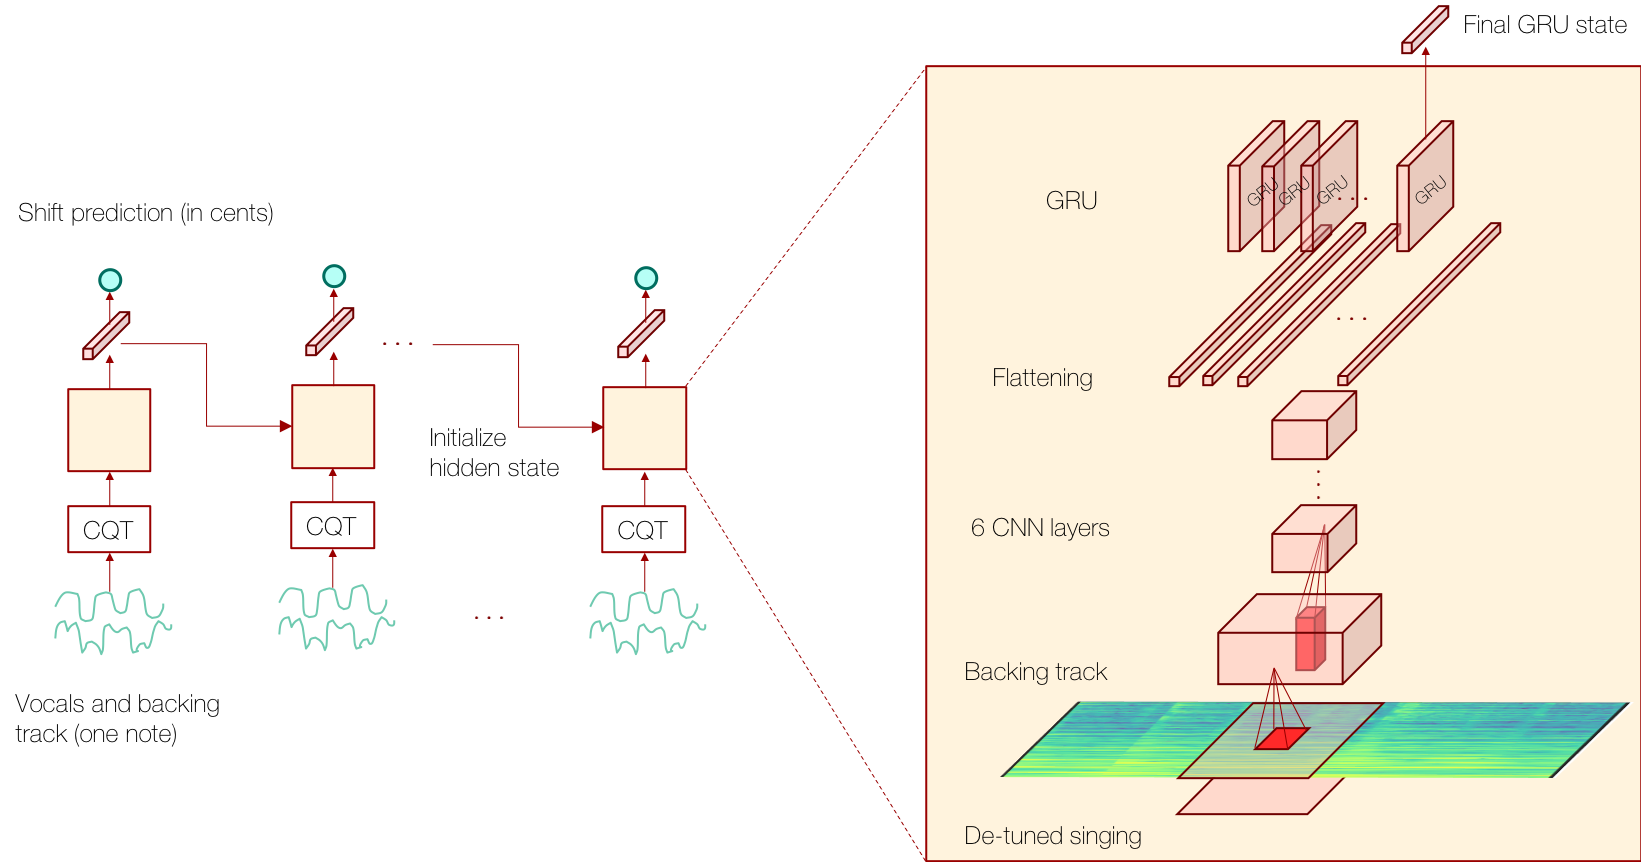
\includegraphics[width=\columnwidth]{images/model_outline.png}
    \caption{Program overview. The program processes one note at a time, and predicts a constant shift for the note's duration. The proposed \gls{dnn} architecture includes convolutional layers for feature extraction followed by \gls{gru}s for sequential processing.}
    \label{fig:model_outline}
\end{figure}

\section{Related work}
%related work
%pitch correction
%- mention antares
The first commercial pitch-correction technique, Antares Auto-Tune \cite{antares:2016}, is also one of the most commonly used. Section \ref{sec:autotune} describes how it is designed. Auto-Tune measures the fundamental frequency of the input monophonic singing recording, then re-synthesizes the pitch-corrected audio signal. In recent work on continuous score-coded pitch correction \cite{salazar2015continuous}, as in Auto-Tune, each vocal note is pitch shifted to the nearest note in a user-input set of pitches (scale) or to the note in the score if it is known. The default musical scale is the equal-tempered scale, in which each pitch $p$ belongs to the set of \gls{midi} pitches $[0, 1, ..., 127]$ and its frequency in Hertz is defined as $440*2^{\frac{p-69}{12}}$. Some users prefer a finer resolution and include more than twelve pitches per octave, or use intervals of varying sizes between pitches. In every case, the fundamental frequency is discretized to a small set of values, around which every note is shifted to be exactly centered. Hence, the pitch shifts tend to ignore a singer's intentional expressive gestures and might not easily apply to musical traditions with different scales or more fluidly varying pitch. The proposed algorithm accommodates a variety of frequencies by letting the fundamental frequency take any value along a continuous scale, and by shifting every note by a constant without modifying internal pitch variation.

%- other pitch correction programs
Recent style-transfer-based work modifies amateur performances to mimic a professional-level performance of the same song. Luo \textit{et al.} proposed to match the pitch contour of the professional-level performance while preserving the spectral envelope of the amateur performance \cite{luo2018singing}. Meanwhile, Yong and Nam proposed to match both the pitch and amplitude envelopes \cite{yong2018singing}. The proposed approach is similar in the sense that it also uses features gathered from high-quality performances \cite{wager2018intonation}. However, the proposed model does not necessitate a ``target" performance of the same song during testing. Instead, it learns from many in-tune singing voice examples and their backing tracks, and then generalizes to unknown songs, while preserving the original singer's style.

\subsection{Music information retrieval}
%pitch detection
%    - pitch detection (ok)
%    - \gls{cqt} (ok)
\gls{mir} research on related tasks such as pitch detection provides a useful background for this thesis. Gomez {\it et al.}\cite{gomez2018deep} provide an overview of recent developments in deep learning for singing processing, ranging from pitch detection to singing separation and synthesis. We focus here on pitch detection as it is particularly relevant to automatic pitch correction. It also aims to extract harmonic patterns from the audio, which correspond to perceived pitch. In the case of pitch detection, the perceived pitches are often manually annotated. 

Bittner \textit{et al.} introduce a fully convolutional \gls{dnn} for polyphonic pitch transcription. The input is the magnitude \gls{hcqt} of the audio. The \gls{cqt} is a time-frequency transformation suitable for a convolutional neural network. It can be contrasted to the Fourier transform, which has linearly spaced center frequencies $f_n = n * \frac{SR}{N}$, where $n$ is the frequency bin index, $SR$ is the sampling rate, and $N$ is the dimension of the transformation space. The \gls{cqt} instead has logarithmically spaced center frequencies $f_j = f_{min} * 2^{\frac{j}{b}}$ where $f_{min}$ is a pre-defined minimum frequency and $b$ determines the number of bins per octave. The fact that the center frequencies are logarithmically spaced results in the audio representation being translationally invariant, meaning that shifting a musical interval up or down will not change the discance between the harmonics in the \gls{cqt}. This enables a \gls{cnn} filter to discover harmonic patterns across the full range of frequencies. Another advantage of the \gls{cqt} representation is that its resolution resembles that of the human auditory system, with high resolution in the lower frequencies and wider bins in the higher frequencies. The downside of using \gls{cqt} is that it cannot benefit from the Fast Fourier transform optimization, so is computationally expensive, $\mathcal{O}(N^2)$ instead of $\mathcal{O}(N \log (N))$. Bittner \textit{et al.} add more resolution by computing multiple, overlapping \gls{cqt}s, each starting at a different frequency. This technique is called \gls{hcqt}. The \gls{cnn} structure includes four lower layers with small filters of dimension $5 \times 5$ or $3 \times 3$ to detect small-scale patterns. The fifth layer, instead, uses a filter that spans an octave of audio. This layer increases the relevant receptive field of each output state---the context in the input \gls{hcqt} it can access---without needing to make the network very deep. The sixth layer uses a $1 \times 1$ filter to combine all the learned features and output a pitch activation map \cite{bittner2017deep}. The \gls{dnn} proposed in this thesis utilizes CNN layers whose structure is closely based on this network. Since the pitch correction task is sensitive even to a small amount of pitch shift, I also choose to use the \gls{cqt} for its finer resolution in the lower frequencies. 

Basaran {\it et al.} add a \gls{gru} layer \cite{chung2014empirical, ChoK2014arxiv} to the pitch detection \gls{cnn} described above in order to model the sequential nature of \cite{basaranmain} audio and music signals. The network estimates the main melody in polyphonic audio signals in the \gls{cqt} representation. 

\subsection{Deep learning}
%deep learning and audio
%    - Amazon paper for CNN + rnn structure + pre-training (ok)
Research in the larger fields of deep learning and audio signal processing also provides a useful background for the task. Wager \textit{et al.} improve the performance of a \gls{dnn} with multiple layers by first training the lower layers on a smaller task, then initializing the corresponding the full network with the trained weights. The network---designed for automatic speech recognition---has a similar structure to the one proposed in this thesis, with linear lower layers for feature extraction followed by recurrent layers for sequential processing \cite{wager2020fully}.
%    - WaveNet
\textit{Wavenet} is a highly expressive model that can synthesize or transform sound at the level of the sample \cite{oord2016wavenet}. The \textit{Wavenet}-based dereverberation network introduced in \cite{su2020hifi} demonstrates that it is able to learn a transformation for a highly complex task. The network is trained in an adversarial manner \cite{goodfellow2014generative} to help the results retain the nature of the original signal. It provides inspiration for moving to a sample-by-sample model. Though this thesis does not include experiments using such a model, the concept of moving to a more fine-grained representation is worth investigating.

\subsection{Audio signal processing}
%pitch shifting
Monophonic pitch detection and transposition techniques provide tools for feature extraction and post-processing. The \gls{pyin} \cite{mauch2014pyin} is used as a benchmark for measuring frequency in monophonic music signals \cite{devaney2020new}. Unlike other state-of-the-art algoritms, including CREPE \cite{kim2018crepe}, its resolution is not limited to a margin such as 20 cents. While this precision is suitable for \gls{mir} tasks such as music recommendations, in the case of musical intonation, 20 cents can make the difference between being in tune or out of tune. The \gls{pyin} algorithm, like the pitch detection algorithm used for Antares Auto-Tune, is based on autocorrelation for periodicity detection. Autocorrelation alone is not always reliable: It might find a stronger periodicity at a harmonic---for example, the octave---or choose a maximum periodicity at value 0, when the signal is not shifted. The \gls{pyin} algorithm is based on the YIN pitch detection algorithm \cite{de2002yin}, which adds steps after the autocorrelation computation to reduce error from 10 per cent to 0.5 per cent. These steps include a weighting of the autocorrelation output to reduce periodicity at harmonics, and a cumulative normalization that discourages selection of the 0-lag periodicity without a need for an arbitrary threshold. It also includes linear interpolation to further refine the pitch estimate. The \gls{pyin} algorithm applies a \gls{hmm} to the output of YIN, using a set of candidate periodicities instead of selecting the maximum one. This results in a smoother output. Both YIN and \gls{pyin} output 0 when they do not detect a period, making the output suitable for voice activity detection and note boundary analysis. The precision of the pitch measurement combined with the voice activity detection make \gls{pyin} ideal for the automatic pitch correction task. As described in \ref{sec:notes}, the \gls{hmm} used in \gls{pyin} inspires the \gls{hmm} explored in this thesis for detecting note boundaries. 

%- PSOLA: TD-PSOLA algorithm 
Another useful tool is \gls{psola}, a pitch shifting algorithm \cite{charpentier1986diphone}. Similarly to YIN, it starts by detecting periodicity in audio. It then splits the audio signal into individual periods, and shifts these slightly in time to produce the effect of shorter or longer periods. It uses cross-fading to avoid clipping. \gls{psola} is suitable for the task because it produces a natural sounding result. Unlike other pitch-shifting techniques such as resampling, it does not modify the structure of the waveform except at the edges of audio windows. This minimizes changes to the formant---the harmonic structure of the sound---so that the timbre is not modified along with the pitch. 
% probabilistic YIN --> also inspires own approach to \gls{hmm} note parsing

\begin{figure*}[t]
\subfigure[]{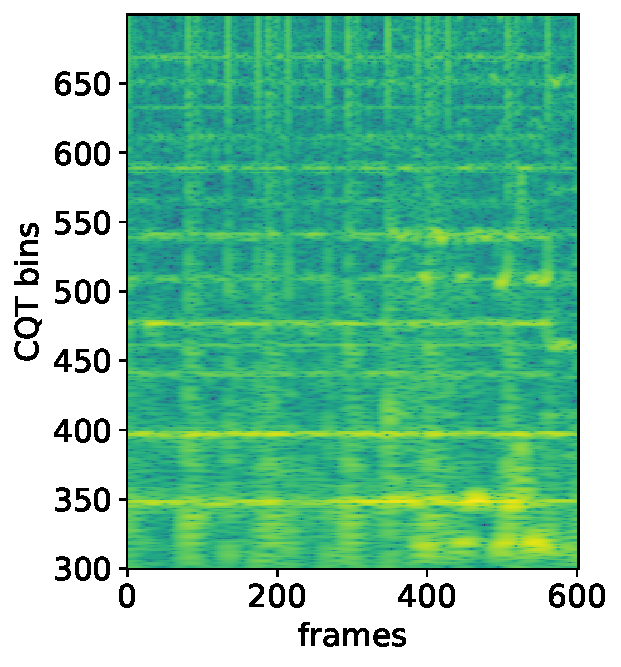
\includegraphics[height=1.625in]{figures/cqt_comparison_1.pdf}}\hspace{-.15in}%\vspace{-.03in}
\subfigure[]{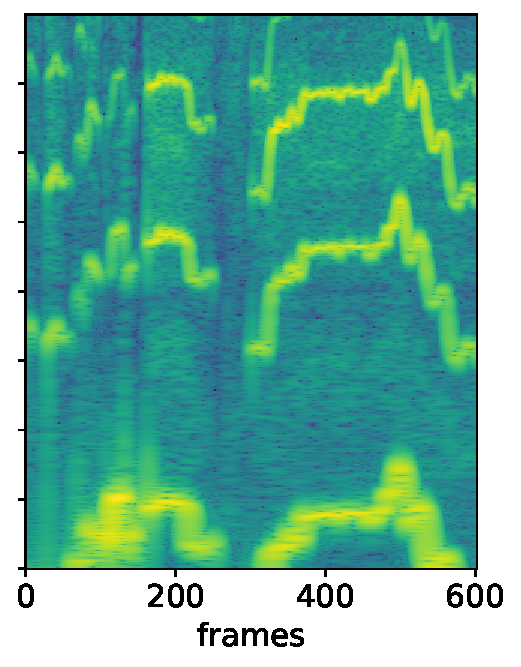
\includegraphics[height=1.625in]{figures/cqt_comparison_2.pdf}}\hspace{-.15in}%\vspace{-.03in}
\subfigure[]{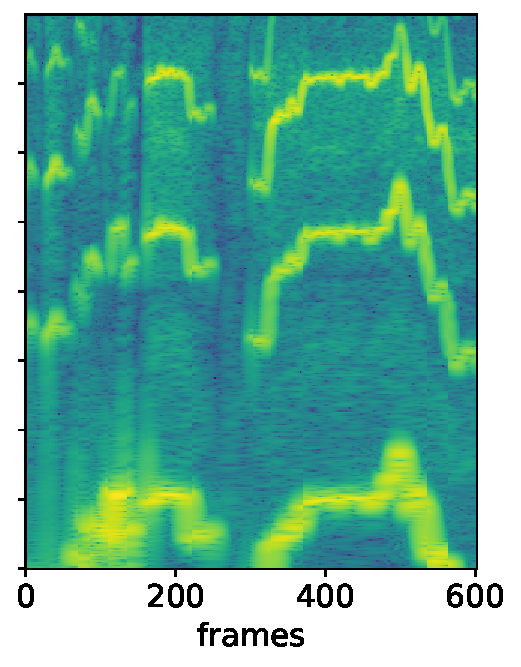
\includegraphics[height=1.625in]{figures/cqt_comparison_3.pdf}}\hspace{-.15in}%\vspace{-.03in}
\subfigure[]{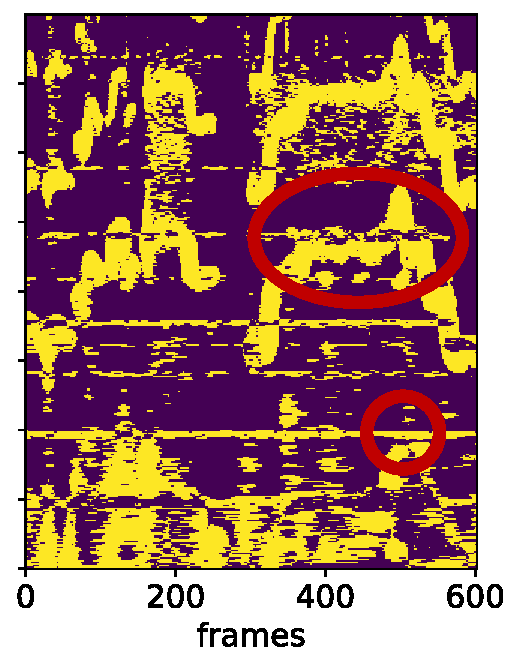
\includegraphics[height=1.625in]{figures/cqt_comparison_4-2.pdf}}\hspace{-.15in}%\vspace{-.03in}
\subfigure[]{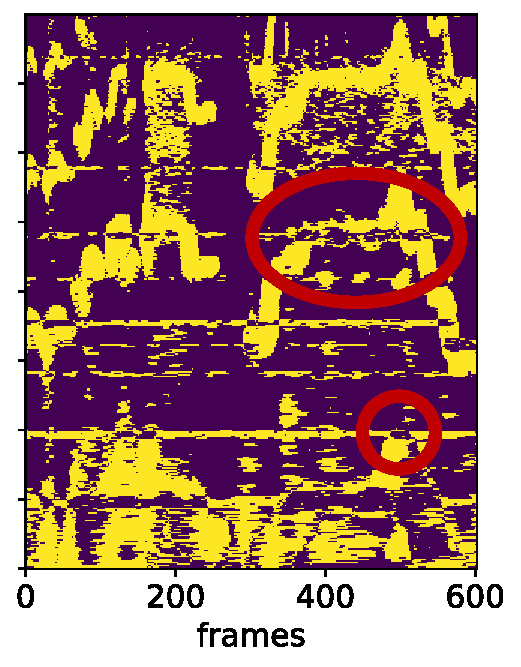
\includegraphics[height=1.625in]{figures/cqt_comparison_5-2.pdf}}\hspace{-.15in}%\vspace{-.03in}
    \caption{
    \gls{cqt} of the vocals and backing tracks computed using Librosa \cite{mcfee2015librosa}. The plot focuses in on frequency bins 300 through 700 out of 1024 for better visibility. (a) shows the \gls{cqt} of the backing track. The horizontal lines are due to constant pitches, which indicates that a chord is being played. (b) and (c) show the \gls{cqt} of the vocals before and after the correction, respectively. (d) and (e) show the superposed vocals and backing track before and after corrections. The \gls{cqt}s are binarized by the mean of their amplitude, which makes the louder components stand out for visibility (see Section \ref{sec:data-format-autotune}). In this example, we see that the correction shifted the pitch of the vocals up and centered it around the desired harmonics of the backing track (red circles).
    }
    \label{fig:model-input-autotune}
\end{figure*}

%Proposed model
\section{The proposed algorithm}
\label{sec:proposed-autotune}
%- harmonic alignment (ok)

\begin{figure}[t!]
    \centering
    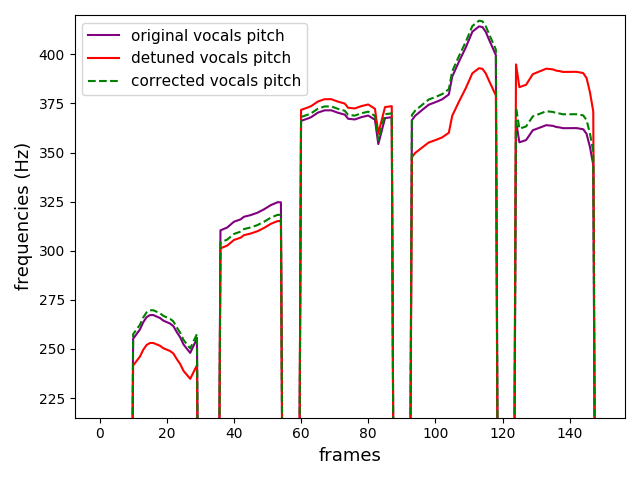
\includegraphics[width=12cm]{images/pitch_before_detuned_after.png}
    \caption{Training technique for the model using synthesized in tune versus out-of-tune data pairs. The program first detunes the original singing. As a result, the measured pitch moves from the purple line to the red line. The deep neural network takes as input the detuned signal, and predicts shifts that will restore the original pitch. The result of the predicted corrections is in green.}
    \label{fig:results}
\end{figure}

The proposed model predicts pitch correction based the \gls{cqt} of the monophonic vocals and the backing track (also called accompaniment). Its structure is built on the assumption that the backing track has clearly identifiable pitches---a chord progression---which serve as a reference for the vocals. The program can then use the harmonic alignment between the vocals and backing tracks to make its predictions. Figure \ref{fig:model-input-autotune} shows the \gls{cqt} of vocals and backing track excerpts of a few notes before and after applying predicted pitch corrections. In the excerpt, the backing track pitches are mostly constant, meaning that a chord is likely being held. After the correction, the vocals appear to be more closely aligned with the backing track, as can be seen in a \gls{cqt} combining the two tracks. The shifts are subtle enough that they are difficult to see in the separate tracks. Note that the algorithm only shifts the vocals, and does not modify the backing track. 

%- supervised training pairs. discuss this in data sec. (ok)
The model is trained in a supervised manner. Training data consists of pairs of performances that are identical except for the vocals pitch. The backing track remains fixed, as it is when the singer performs in a karaoke setting. The input-target pairs, while required to train the model, are difficult to come across naturally. Hence, I synthesize them by detuning high-quality singing performances to construct the input signals, and then train the \gls{dnn} to predict the shifts that recover the original pitches. Section \ref{sec:data-format-autotune} describes the de-tuning process.
\begin{figure}[t!]
    \centering
    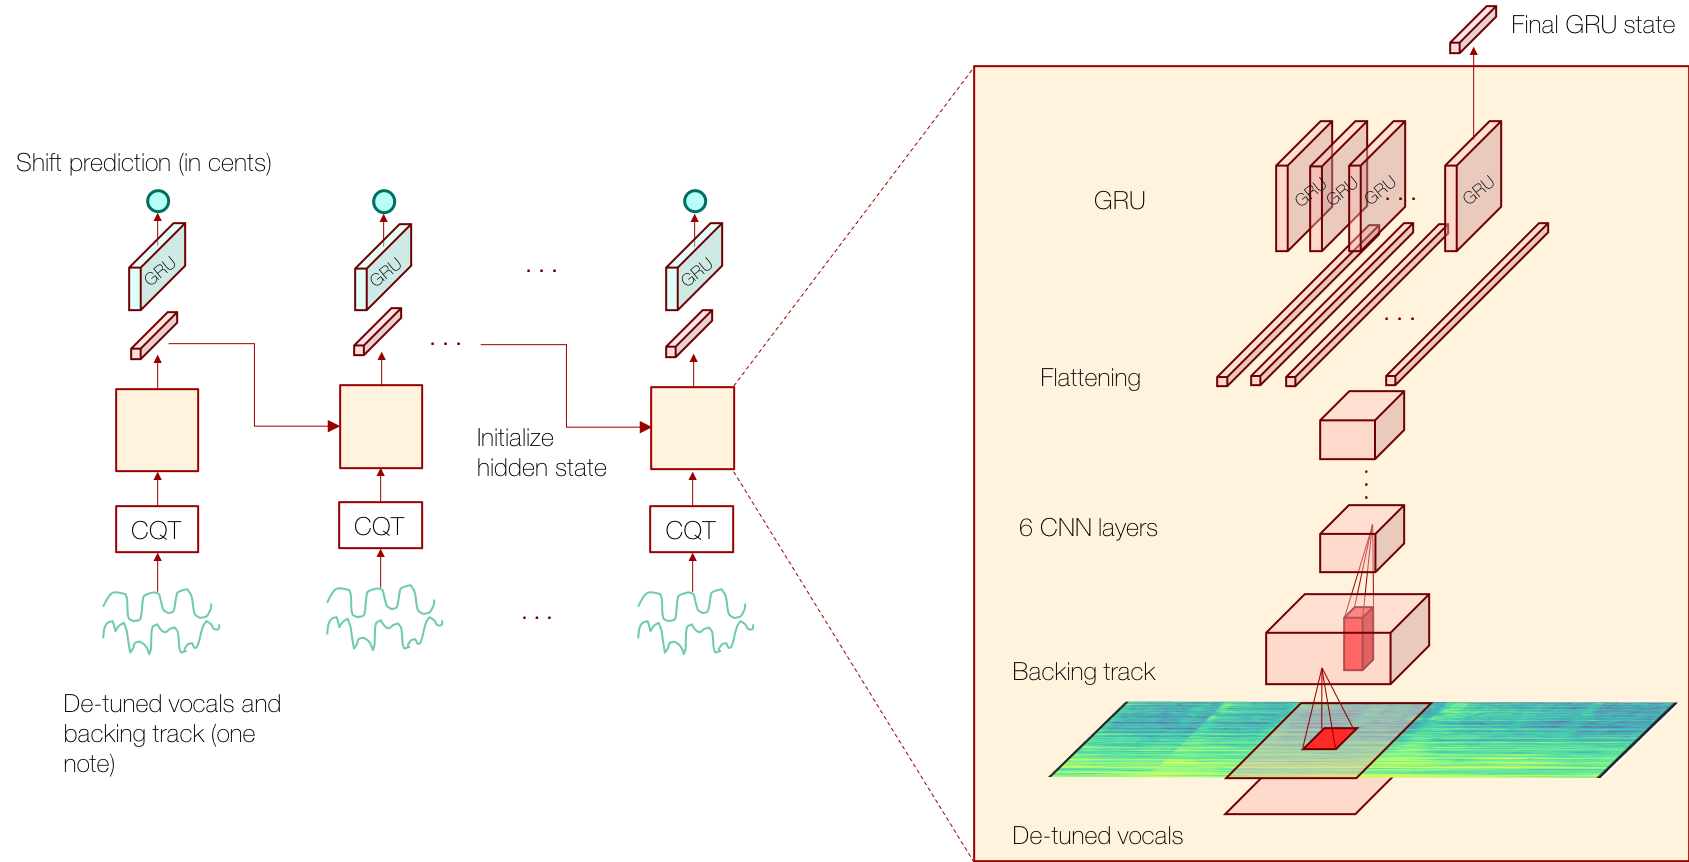
\includegraphics[width=\columnwidth]{images/model_outline_extension.png}
    \caption{Model architecture with extension layer. A \gls{gru} sequentially processes the outputs for each note from the original \gls{dnn}  and is followed by a linear layer that outputs note-wise shifts.}
    \label{fig:model_outline_extended}
\end{figure}
%    - applies to any culture it is trained on
%- time-frequency representation overview
%    - \gls{cqt}

%- note splitting
%    - Discretization for control, constant shift
\subsection{Note-by-note processing}
\label{sec:notes}
A strong assumption behind the proposed algorithm design is that a singer targets a specific frequency per note, around which all pitch variations are centered. Given this assumption, the network corrects the pitch of one note by shifting all frames included in it by a constant. The first step to processing the song note by note is to detect the note boundaries from the original singing performance. I choose not to use a musical score, first, because this makes the program usable in the many situations where no score is available, second, because this avoids inconsistent note boundaries due to alignment errors or improvisation. I tested three different approaches to score-free detection of note boundaries. Their respective outputs can be visualized in Figure \ref{fig:note-parsing}.
\begin{figure}[t!]
    \centering
    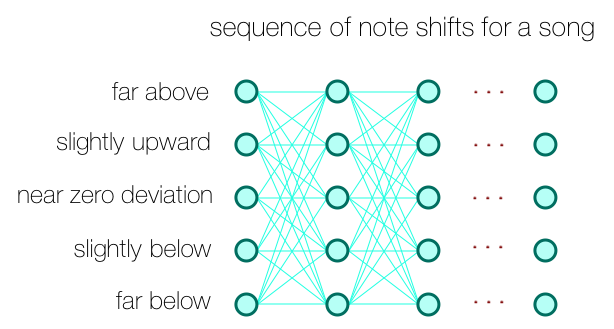
\includegraphics[width=8cm]{images/note_detuning_hmm.png}
    \caption{Note de-tuning Hidden Markov Model. The approximate de-tuning amount per note is defined in the hidden states. The exact de-tuning is sampled from the state using a Gaussian distribution,.}
    \label{fig:detuning_hmm}
\end{figure}

\begin{figure}[h]
    \centering
    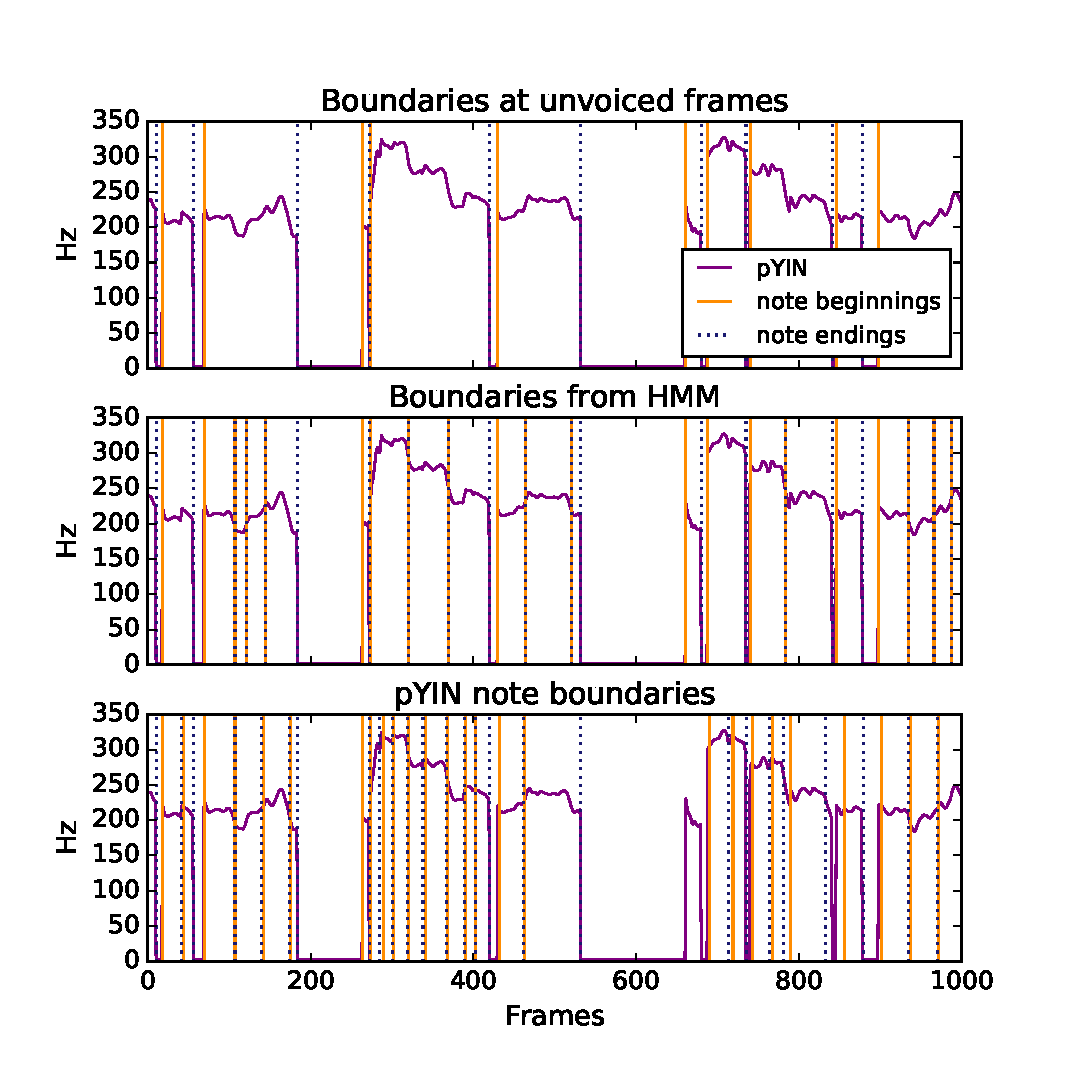
\includegraphics[width=\columnwidth]{figures/note_parse_comparison_attention_5.eps}
    \caption{Comparison of three different note boundary detection outputs for an excerpt from \textit{Attention} by Charlie Puth. The purple line shows the \gls{pyin} frame-wise pitch contour. The vertical lines show the note boundaries. The first and second approaches use the frame-wise \gls{pyin} pitch output. The first approach assigns note boundaries at the beginnings and ends of unvoiced sections. The second approach fits a Gaussian \gls{hmm} to the pitch contour, and uses the hidden state sequence of equal-tempered scale frequencies along with unvoiced frames to assign boundaries. The third one uses the \gls{pyin} note-wise output. In this example, the unvoiced frame approach fails to split some legato passages into individual notes and the \gls{pyin} note approach is the most sensitive, assigning the largest number of notes. Sometimes this is musically relevant: for example, the lyrics in the three-step descending sequence around frames 300 to 400 are ``knew-that-I, knew-that-I, knew-that-I'', splitting each step into three musical events. The \gls{pyin} note detection detects these boundaries. However, it misses some notes---for example, the first note after frame 600---and its boundaries are not exactly aligned with the frames that switch between being voiced and unvoiced---for example, in multiple locations between frames 800 and 900.}
    \label{fig:note-parsing}
\end{figure}

The first, which produced the best result, was to define every transition silence as a note boundary. To this end, I analyzed the vocals pitch using the frame-wise \gls{pyin} algorithm, implemented as a Vamp plugin in \cite{cannam2010sonic}. The frame-wise pitch is set to 0 for unvoiced frames, which makes it possible to easily treat transitions between voiced and unvoiced frames as note boundaries. A small amount of smoothing was required to avoid glitches in the case where a single frame had value 0. The advantage of this technique is that it minimizes artifacts during shifting. Any discontinuities arising due to pitch shifting a section of an audio recording are insignificant because the audio is silent at the discontinuity points. The disadvantage is that this note parsing technique fails to split notes when they are connected, though this is common in \textit{legato} melodies. This means that if one part of a legato passage is out of tune and another part isn't, a shift that would correct the out-of-tune part would de-tune the other part.

The second approach, which turned out to be too error-prone for the task of automatic pitch correction, was to use the note-wise \gls{pyin} plugin available as an extension to the original frame-level pitch detection algorithm algorithm. This program is useful for melody detection, but I found that it did not always start and end notes at exactly the right frame for minimizing discontinuity. It often left small gaps between the end of one note and the beginning of the next one, making it difficult to determine what to do with these unaccounted frames. It also tended to be rather sensitive, converting pitch bending into two discrete notes. Any undesirable splitting of notes can have a significant impact on the ability of the model to perform reliably well. If a part of a note is separated from the rest and shifted in a different direction, the unnatural result can be displeasing enough to make a whole excerpt sound bad to the listeners.

The third approach assigns note boundaries to the vocal track using a Gaussian \gls{hmm} applied to the frame-wise \gls{pyin} pitch contour. This approach combines the reliable output of \gls{pyin} with a customized note parsing technique. The hidden states in the \gls{hmm} are the equal-tempered scale frequencies within the range of the minimum and maximum value in the pitch contour, $440 * 2^{\frac{p - 69}{12}}$, where $p \in [21, 108]$, the standard \gls{midi} range. They also include 0 for silence or unvoiced frames. The standard deviations correspond to the absolute difference in pitch between each equal-tempered scale frequency, leaving much room for the frame-wise pitch to deviate from the scale. The transition matrix is set to 0.001 everywhere except in the diagonal, which makes each row sum to 1. The starting probabilities are uniformly distributed. Fitting this model assigns a \textit{note} state to each frame and provides boundaries both between \textit{legato} notes and between unvoiced and voiced sections. The potential shortcoming of this approach is that it relies on the definition of a discretized scale. I note that it would be possible to use a more fine grained scale if working with a musical style that is not based on the equal-tempered scale---for example, use 22 subdivision of the octave for Classical Indian music. I used the equal-tempered scale here because the dataset I worked with was mostly made of popular music that used that scale.  

%    - hmm for note splitting (ok)
%        - now set up for equal-tempered for simplicity (ok)
%        - could set up a fine-grained scale, 22 notes as %in raga, or any other customization (ok)
% could, in the future, try WaveNet (ok)
%- model structure with CNN and RNN
\subsection{Neural network structure}
This section describes two versions of the proposed algorithm. The second version is an extension of the first, designed to include more temporal context across notes. The first version of the network consists of six stacked convolutional layers followed by a \gls{gru} layer. The network architecture is illustrated in Figure \ref{fig:model_outline}. The last output of the \gls{gru} is fed to a dense layer that predicts a single scalar output, the note-level pitch shift. The convolutional filters pre-process the spectrogram tensor, reducing its dimensionality while also learning abstract features. Next, the \gls{gru}---from which the network only uses the last output---reduces the representation of a variable-length note to a fixed-length vector. Finally, the dense layer predicts the pitch shift in the approximate range of $-1$ to $1$, which is mapped to a semitone in either direction, or $-100$ to $100$ cents. The activation after each convolutional layer is the \gls{relu} \cite{he2015delving}. There is no nonlinear activation after the final dense layer, as this might encourage nonzero values. One example is the hyperbolic tangent function, which tends to move values closer to $-1$ or $1$ and away from 0. 

The \gls{gru} recurrent structure is a way for the model to analyze the singer's note contour, which can last from a split second to multiple seconds, while smoothing over unvoiced or noisy sections. This is crucial because the algorithm is expected to rely on aligning harmonics, which only occur in pitched sounds. Another advantage of using the \gls{gru} is that the hidden state output by one note can initialize the hidden state for the following note, passing along some information about the previous notes. Even when using the simplest possible detuning model, which shifts every pitch by an independent amount, we can assume that some information from past notes (e.g. from the backing track) is useful.

\begin{table}[t]
  \begin{center}
    \caption{The proposed network architecture.}
    \begin{tabular}{|c||c|c|c|c|}
    \hline
      & Conv1 & Conv2 & Conv3 & Conv4 \\
      \hline
      \#Filters/Units & 128 & 64 & 64 & 64 \\
      Filter size & (5, 5) & (5, 5) & (3, 3) & (3, 3) \\
      Stride & (1, 2) & (1, 2) & (2, 2) & (1, 1) \\
      Padding & (2, 2) & (2, 2) & (1, 1) & (1, 1) \\
      \hline
      & Conv5 & Conv6 & \gls{gru} & Linear \\
      \hline
      \#Filters/Units & 8 & 1 & 64 & 1 \\
      Filter size & (48, 1) & (1, 1) & & \\
      Stride & (1, 1) & (1, 1) & & \\
      Padding & (24, 1) & (0, 0) & & \\
      \hline
    \end{tabular}
    \vspace{-.1in}
    \label{tab:network}
  \end{center}
\end{table}

%- option of adding additional song-rnn
The second version of the algorithm is designed to enable the model to include more temporal context. As shown in Figure \ref{fig:model_outline_extended}, the final dense layer is replaced by a second \gls{gru} that takes as input the sequence of note representations output one-by-one by the first \gls{gru}. It finally applies a dense layer to the full sequence to output a song-level prediction sequence. This version has the potential to reach farther back in time, and include information from the chord progression in the backing track and long-term melodic patterns in the vocals. The downside of this model design is that the \gls{dnn} is deeper, which makes it more difficult to train. 

% - predict shift, apply it later (ok)
Table \ref{tab:network} displays the structure of the proposed network without the song-level \gls{gru} extension. The feature extraction layers are convolutional, which is common for image processing. The input to the model is in spectrogram format, which resembles an image, except for the fact that its meaning is different along the time and frequency axes. In image progessing, dimensions reduction techniques like max pooling are common. These techniques treat the x and y axes in the same way, which we wish to avoid. To preserve the frequency patterns axis, the proposed approach instead uses strides of two only in the time axis in three of the convolutional layers, as done successfully for the task of learning latent representations for speech generation and transformation in \cite{hsu2017learning}. The third layer also includes a stride along the frequency axis, but this occurs only in one layer to not lose too much information. The fifth convolutional layer has a filter of size 48 in the frequency domain, which captures frequency relationships in a larger range of the \gls{cqt}, as shown to be successful in \cite{bittner2017deep} and \cite{hsu2017learning}. 
The error function is the \gls{mse} between the pitch shift estimate and ground truth over the full sequence of notes in a performance. The \gls{mse} corresponds to the error in cents using the formula $\left|\text{cent error}\right| = 100 * \sqrt{\text{\gls{mse}}}$. % When training and testing the program, \gls{mse} is the only objective accuracy metric, though we have audio examples for an informal evaluation. A subjective test provides a qualitative evaluation when applying automatic pitch correction to real-world singing examples.

\subsubsection{Applying the predicted pitch corrections}
Once the program has output pitch correction predictions, these are applied to the vocals. The \gls{psola} algorithm provides a natural sounding output with few artifacts. The shifting is constant across note, and subtle cross-fading is applied between legato notes---in between which there is no silence---to avoid glitches at the boundaries.

%- post-processing focus
\subsection{Post processing versus real time}
The neural network introduced in this thesis is not explicitly designed to work in real time. First, the algorithm is designed for post-processing plug-ins such as are found in music apps like Smule. Second, the task of automatic pitch correction is challenging enough even given abundant computation time, so I choose to leave real-time applications to future work. 

Even in its current form, though, the model might be adaptable to near-real-time processing as it only uses information from previous notes to make a prediction for the current note. Even within a note, it processes one frame at a time in order. The challenge would be to make the data pre-processing---involving pitch detection and feature extraction---fast enough. 

%Dataset
%- Intonation introduction, refer to chapter (ok)
%    - genres in the dataset (ok)
%Real-world dataset (ok)
%- real-world set for testing (ok)
\subsection{Dataset}
\label{sec:dataset-autotune}
During my internship with Smule, Inc, a company that offers a singing app for smartphone, my team and I constructed a training dataset by deriving from the ``Intonation" dataset \cite{wager2018intonation}, which is assumed to be a collection of in-tune singing voice tracks. A detailed description of the dataset, including instructions on how to access it, is available in Chapter \ref{chap:thesis-damp}. The 4702 separate vocal tracks in the dataset are mostly of Western popular music, collected at Smule for good intonation. While browsing the dataset, I also discovered a few tracks of Blues; Western Classical music; Latin, Japanese, and Indian popular music, Country; and Rock. The songs are mostly based on the equal-tempered scale, but contain a wide variety of pitch deviation patterns from the scale. I discuss the measured pitch distribution in Chapter \ref{chap:thesis-damp}. While these real-world recordings contain some artifacts, no particular signal processing---e.g. denoising or filtering---has been applied to them. Each recording contains one minute of a performance, starting 30 seconds into the song. Although they are assumed to be in tune, this is not always exactly the case as the users are not necessarily professional singers. Overall, the sung pitch is sounds quite accurate and aligns reasonably well in timing and in pitch with the known musical score. Note when compared with the intended pitch. Hence, we can treat this paper as a proof of concept. The model can be trained on professional singing for best results.

Based on the metadata for each track indicating the backing track and user index, the dataset is split into 4561 training performances, 49 validation performances, and 64 test performances. The training set contains 709 backing tracks performed by 3468 different users, while the validation set is with 17 tracks sung by 43 users and the test set is with 16 sung by 62. There is no overlap in the backing tracks across the three sets. Overlap exists in the singer ID between the training and validation sets, but not with the test set. 

%For a subjective listening test, I also create another real-world test set using the test backing tracks. Originally, 8 volunteers sang along with them outside of Smule. Singing experience ranged from beginner to semi-professional. The singers chose what to sing, and selected a total of 9 different arrangements. The dataset consisted of a total of 24 performances. The dataset later grew to N performances to increase its size and diversity of voices and singing styles. Instructions during the recording session included singing once in a normal manner and once mimicking an imaginary out-of-tune karaoke singer. The reason for this is that it is interesting to examine how the algorithm performs both with performances that are already quite accurate, and with performances that are severely out of tune. Singers familiarized themselves with their chosen songs at their own pace over the course of a few days before the recording session. They used the Smule interface, which provides the lyrics and the piano roll score for reference. During the performance, they listened to the backing track through headphones so that it would not interfere with the vocals recording.

%De-tuning process
\subsection{The detuning process}
As introduced in Section \ref{sec:proposed-autotune}, the \gls{dnn} is trained in a supervised manner. An input data sample consists of an out-of-tune performance, and the target consists of the note-wise shifts that should be applied to the vocals track to make it sound in tune. This type of pair is difficult to come across, unless one manually labels the corrections for every note in hundreds or in thousands of performances. The proposed approach to constructing training examples is to synthesize de-tuned examples. Singing performances from the ``Intonation'' dataset are de-tuned by shifting every note up or down and recording the amount of shift as the target. The synthetic pitch deviations are limited to approximately one semitone (100 cents) in either direction, a larger interval than the standard score-free approach of snapping to the nearest pitch, which limits the shift to 50 cents. In practice, it prevents errors in cases where the required shift is greater than 50, but can lead to degradation of the prediction accuracy on a too badly detuned input. 

To detune the training data, the program shifts the magnitude \gls{cqt} up or down. This is expected to not produce too noticeable artifacts that the program could learn instead of the pitch relationships. The one issue is formant shifting, but this is not a big concern when only shifting by $\pm$100 cents or less. I experimented with shifting the training data using \gls{psola}, but this did not produce noticeably better convergence, and increased the computational complexity due to the need to compute autocorrelation instead of simply shifting a matrix. 

\subsubsection{De-tuning distributions}
%- data de-tuning, different versions (ok)
%    - runif (ok)
%    - hmm (ok)
%        - MIR-1K (ok)
% rnn (ok)
The de-tuning process described in the previous section requires assigning a distribution to the random shifts. Choosing a proper distribution involves balancing exposing the model to a wide variety of errors with ensuring it also is exposed to small deviations. A too spread distribution risks causing the model to frequenly apply large corrections, and produce noticeable errors. 

I experimented with two distributions. The first is the random uniform distribution in the range [-100, 100] cents, adjusted to the logarithmic scale of cents so that the shift of the \gls{cqt} spectrogram is linear. Random uniformly distributed shifts are very simple to implement, and provide the model with plenty of examples of a wide variety of shifts, ranging from zero---which is useful, because singers are not likely to sing every note out of tune---to large ones. The downside is that this de-tuning technique is not based on real intonation patterns in out-of-tune singing. Furthermore, it is based on the strong and likely incorrect assumption that the detuning for every notes is independent from that of other notes.

A Gaussian \gls{hmm} addresses both of the shortcomings of the random uniform distribution in a simple manner. \gls{hmm} states represent deviation levels, while the Gaussian distribution provides variance. The \gls{hmm} structure is illustrated in Figure \ref{fig:detuning_hmm}. The \gls{hmm} is trained on real-world singing examples in the publicly available MIR-1K dataset of karaoke performances \cite{hsu2009improvement}. The proposed \gls{hmm} outputs deviations in cents from the equal-tempered scale. These deviations are represented as the difference between the equal-tempered frequency output by the \gls{hmm} used to parse notes, described in Section \ref{sec:notes}, and the median of the measured frame-wide \gls{pyin} pitch. As before, the equal-tempered scale can be replaced with any other division of the octave. The proposed model uses five hidden states, but the number is arbitrarily chosen and can be replaced by a different value.  Sampling from this \gls{hmm} produces sequences of pitch deviations that are based on real-world deviations and are not completely independent across notes.

To address the issue that all deviations will be 50 cents or less, because the distance to the nearest scale degree will never be greater than this, the \gls{midi} pitch is moved by a semitone 5 per cent of the time across the median measured pitch, increasing the range to 100 cents. 5 per cent was another arbitrary choice, but the use of \gls{hmm} is still expected to produce a slightly more accurate pitch behavior representation than the random uniform distribution.

The parameters learned from the MIR-1K dataset are in Table \ref{tab:detuning-hmm}. The means show a state very close to the equal-tempered scale, at 3, two that are offset by a few cents---one in each direction---and two that are more than a quarter tone away. I note that singers were very likely to start close to an equal-tempered scale degree, and almost never started far off. They also didn't tend to stay far off, as the transition probabilities from a larger deviation to a larger deviation are the smallest.\footnote{I later realized that the pitch detection was based on mixed MIR-1K signals, which included the accompaniment. This resulted in a more spread and noisy distribution, but I believe this larger spread was useful for training the model to address larger shifts.} One should note that these parameters include the occasional shifts of the note across the median pitch. Despite this modification, the distribution is slightly less spread than the random uniform option, as shows in Chapter \ref{chap:results}, Figure \ref{fig:test-comparison}.

\begin{table}[t]
  \begin{center}
    \begin{tabular}{|c|c|c|c|}
    \hline
      $\mu$ & $\sigma$ & $p_{start}$ & $p_{trans}$ \\
      \hline
      &&& \\
      $\left[ \begin{array}{c} 52 \\  13 \\3\\-8\\-73 \end{array}\right]$
      & $\left[ \begin{array}{c} 31  \\ 25\\16\\25\\24 \end{array}\right]$
      & $\left[ \begin{array}{c} 0.1  \\ 9\\76\\15\\0.1 \end{array}\right]$
      & $\left[ \begin{array}{ccccc} 4 & 30 & 30 & 35 & 1  \\ 13&27&30&24&5\\24&17&22&15&23\\16&25&28&23&7\\3&36&30&30&0 \end{array}\right]$  \\
      &&& \\
      \hline
    \end{tabular}
    \label{tab:detuning-hmm}
    \caption{The de-tuning Gaussian \gls{hmm} parameters fitted to the MIR-1K dataset. The first column shows the means, or hidden states, and the second column shows the standard deviations. The final two columns show the start and transition probabilities. All parameters are in cents, a logarithmic measure, and rounded to the nearest integer, except for zeros, which are set to $0.1$ to show that no transition had zero probability.}
  \end{center}
\end{table}

The \gls{hmm} model pitch deviation is not the most complex model that could be used for the task. It could be replaced by a RNN that uses additional information, such as absolute frequency---given that a singer might be more likely to sing sharp or flat based on the register---or spectral information. One could go another step further and synthesize out-of-tune singing using a WaveNet and/or adversarial training.

\subsection{Data pre-processing details}
\label{sec:data-format-autotune}
The audio signals are normalized, then transformed using the \gls{cqt}. The \gls{cqt} covers 5.5 octaves with a resolution of 16 bins per semitone. The lowest frequency is 125 Hz. The top and bottom 16 bins are used as a buffer for pitch shifting, then truncated so that every input has dimension 1024. The frame size spans 92 ms and the hop size 11 ms. The vocals and backing track \gls{cqt}s form two input channels to the neural network. In previous work, I experimented with using a third channel that would help bring out the contrast between the first two channels. I binarized the two \gls{cqt} spectrograms using the mean modulus as a threshold, a technique used in computer vision \cite{sezgin2004survey}. I then took the bitwise disagreement of the two matrices based on the expectation that the in-tune singing voice, better aligned with the backing track, would cancel out more harmonic peaks than the out-of-tune tracks. Figure \ref{fig:model-input-autotune} illustrates the three channels. It includes the binarized \gls{cqt} before and after shifting though the third channel was ultimately left out, because it helps visualize the shift. Surprisingly, though the convergence with the third channel was better for multiple epochs, the loss with two channels ultimately dropped below its counterpart. The difference took long enough to appear that I only discovered it because I had left two models training for additional time despite having already concluded that the third channel improved the results. 
%- \gls{cqt} parameters, etc… (ok)
%- tried third channel, did not help (ok)
%- tried the binary channel but did not help (plot)? (ok)
%- Tried \gls{psola}, expensive but not better (ok)

%Experimental setup
\section{Experimental configuration}
\label{sec:experiments-autotune}
\subsection{Training setup}
The program uses the Adam optimizer \cite{kingma2014adam}. It processes one note at a time as a minibatch of seven differently pitch-shifted versions. It does not include batch normalization because the different versions of the same note are not \textit{i.i.d}. When using the second \gls{gru} layer that bases the prediction on the sequence of notes, the outputs for each note are stored, then input to the \gls{gru}. 

The program applies gradient clipping \cite{pascanu2013difficulty} with a threshold of 100. It reports validation loss every 500 songs and save the model with the best result along with the latest one. 
%- loss function, etc… (ok)
%- Adam (ok)
\subsection{Initialization}
The convolutional parameters are initialized using He \cite{he2015delving}, and the \gls{gru} hidden state of the first note of every song is initialized using a normal distribution with $\mu=0$ and $sd=0.0001$. The hidden state of the note sequence \gls{gru} is initialized in the same way. When using the note sequence \gls{gru}, the weights from the note-by-note model can optionally be used to initialize the lower layers. These lower layers can also be fixed for an epoch before being trained all the network parameters. 

\subsection{Experiments}
\label{sec:experiment-list}
In this thesis, I report test results on a set of different configurations, listed in Table \ref{table:experiments}. Note that I only report configurations that showed the strongest convergence. First, I compare note parsing techniques and de-tuning techniques when training the smaller version of the model. I examine various learning rates. For the best performing models, I add the song-level \gls{gru} extension to check whether the deeper neural network performs better. I train the extended model either from scratch or initializing feature extraction parameters with the values learned for the smaller model. In the latter case, I freeze the pre-trained weights for one epoch. This technique was shown successful in previous work, e.g., \cite{wager2020fully}. For each model, I report results either with learning rate 0.00001 or 0.000005, based on which setting converged best. Other learning rates did not converge.

\begin{table*}
\centering
\begin{tabularx}{\columnwidth}{ |X|X|X|X|X| } 
\hline
\multicolumn{5}{|c|}{\textbf{Experiment settings}}\\
\hline\hline
\textbf{Note parsing} & \textbf{De-tuning} & \textbf{Learning rate} & \textbf{Extension} & \textbf{Initialization} \\
\hline\hline
Silence & Uniform & 0.00001 & No & He, Gauss \\
\hline
Silence & \gls{hmm} & 0.000005 & No & He, Gauss\\ 
\hline
\gls{hmm} & \gls{hmm} & 0.00001 & No & He, Gauss\\ 
\hline
Silence & Uniform & 0.000005 & Yes & pre-trained, Gauss\\
\hline
Silence & \gls{hmm} & 0.000005 & Yes & He, Gauss\\ 
\hline
Silence & \gls{hmm} & 0.000005 & Yes & pre-trained, Gauss\\ 
\hline
\end{tabularx}
\label{table:experiments}
\caption{The \textit{Note parsing} column indicates whether the note boundaries were assigned based on silent \gls{pyin} frames or based on state changes in the \gls{hmm} assigning a scale degree to each frame. The \textit{De-tuning} column indicates whether the de-tuning distribution was random uniform or sampled from the \gls{hmm} trained on MIR-1K. The \textit{Extension} refers to whether the song-level \gls{gru} is added to the model architecture. Finally, the \textit{Initialization} column provides the distributions used to initialize the parameters, and whether the feature extraction layers were initialized using pre-trained parameters from the model without extension.}
\end{table*}

%\begin{table*}
%\centering
%\begin{tabularx}{\columnwidth}{ |X|X|X|X| } 
%\hline
%\multicolumn{4}{|c|}{\textbf{Experiment settings}}\\
%\hline\hline
%\textbf{Model names} & \textbf{Learning rate} & \textbf{Initialization} & \textbf{De-tuning} \\
%\hline\hline
%Note-runif-1e-5 & 0.00001  & He, Gauss & Uniform \\
%\hline
%Note-runif-5e-6 & 0.000005 & He, Gauss & Uniform \\
%\hline
%Note-\gls{hmm}-1e-5 & 0.00001 & He, Gauss & \gls{hmm} \\ 
%\hline
%Song-runif-1e-5 &  0.00001 & He, Gauss & Uniform \\ 
%\hline
%Song-runif-5e-6 &  0.000005 & He, Gauss& Uniform \\ 
%\hline
%Song-\gls{hmm}-1e-5 & 0.00001 & He, Gauss & \gls{hmm} \\ 
%\hline
%Song-\gls{hmm}-5e-6 & 0.000005 & He, Gauss & \gls{hmm} \\ 
%\hline
%Song-\gls{hmm}-pretrain-1e-5 & 0.00001 & ``Note-\gls{hmm}-1e-5'' weights, Gauss & \gls{hmm} \\ 
%\hline
%Song-runif-pretrain-1e-5 & 0.00001 & ``Note-\gls{hmm}-1e-5'' weights, Gauss & Uniform\\
%\hline
%\end{tabularx}
%\label{table:experiments}
%\caption{List of experiments}
%\end{table*}

%- initialization of weights
%- pre-training
%Experiments
%- runif by note
%- hmm by note
%- runif by sequence
%- hmm by sequence
%- learning rates
%- + pre-training

%%%%%%%%%%%%%%%%
% Chapter 5
%%%%%%%%%%%%%%%%

\chapter{``Intonation'': A dataset of quality vocal performances refined by spectral clustering on pitch congruence}
\label{chap:thesis-damp}
%Introduction
%- dataset of musical performances
%    - how to gain access
%- semi-supervised approach that can be used for other data %collection tasks (describe in next section)
%- provides an analysis in light of chapter 2
This chapter describes the collection process of the ``Intonation'' dataset used in this thesis\footnote{This work was supported by the internship program at Smule, Inc.}. The ``Intonation'' dataset consists of amateur vocal performances with a tendency for good intonation, collected from Smule, Inc. The dataset can be used for music information retrieval tasks such as automatic pitch correction, query by humming, and singing style analysis. It is publicly available.\footnote{The dataset and detailed description of the contents are available upon request via \url{https://ccrma.stanford.edu/damp}.} I describe a semi-supervised approach to selecting the audio recordings from a larger collection of performances based on intonation patterns. The approach can be applied in other situations where a researcher needs to extract a subset of data samples from a large database. A comparison of the ``Intonation'' dataset and the remaining collection of performances shows that the two have different intonation behavior distributions. I also analyze the ``Intonation'' dataset to check whether its amateur performances of mostly Western popular music show similar tendencies to those described in studies in Chapter \ref{chap:intonation}. 

%Need for music datasets
%- semi-supervised approach
\section{Datasets for music research}
Useful datasets have been made available for certain research topics in the fields of music information retrieval and audio. These include sound event detection \cite{Mesaros2018_DCASE}, source separation \cite{SiSEC17}, and recommendations \cite{bertin2011million}. Sometimes, though, the best dataset available for a topic is huge and difficult to process. A large collection of audio recordings is available, but the recordings with suitable characteristics for the given analysis form a smaller subset of the dataset. The filtering process to extract the desired samples can be labor intensive, requiring that the researcher select the samples with the desired features, which may or may not be labeled and can be hard to model. One way to approach this selection process is to automate it using feature engineering and clustering. 

This chapter provides an example of a semi-automatic process for the task of searching through a large database of amateur karaoke performances for samples with a tendency for good musical intonation. The need for this task arose when designing a machine-learning model to predict pitch correction. The task requires selecting performances that were in tune enough but not those that were out of tune or contained little singing. Note that this task requires quantifying the concept of singing in tune. As described in Chapters \ref{chap:intonation} and \ref{chap:tech-background}, the concept is not obvious to model directly. A semi-supervised approach makes it possible to avoid creating an explicit definition of in tune. We first extracted musical intonation features from each performance, then applied spectral clustering to them and subjectively choose clusters that sound in tune by listening to samples from each. We also introduced the resulting dataset and an analysis of the intonation tendencies of its performances. Though I present this approach for the automatic pitch correction task, it can be adapted to other tasks, datasets, and features.

\begin{figure*}[h!]
    \subfigure{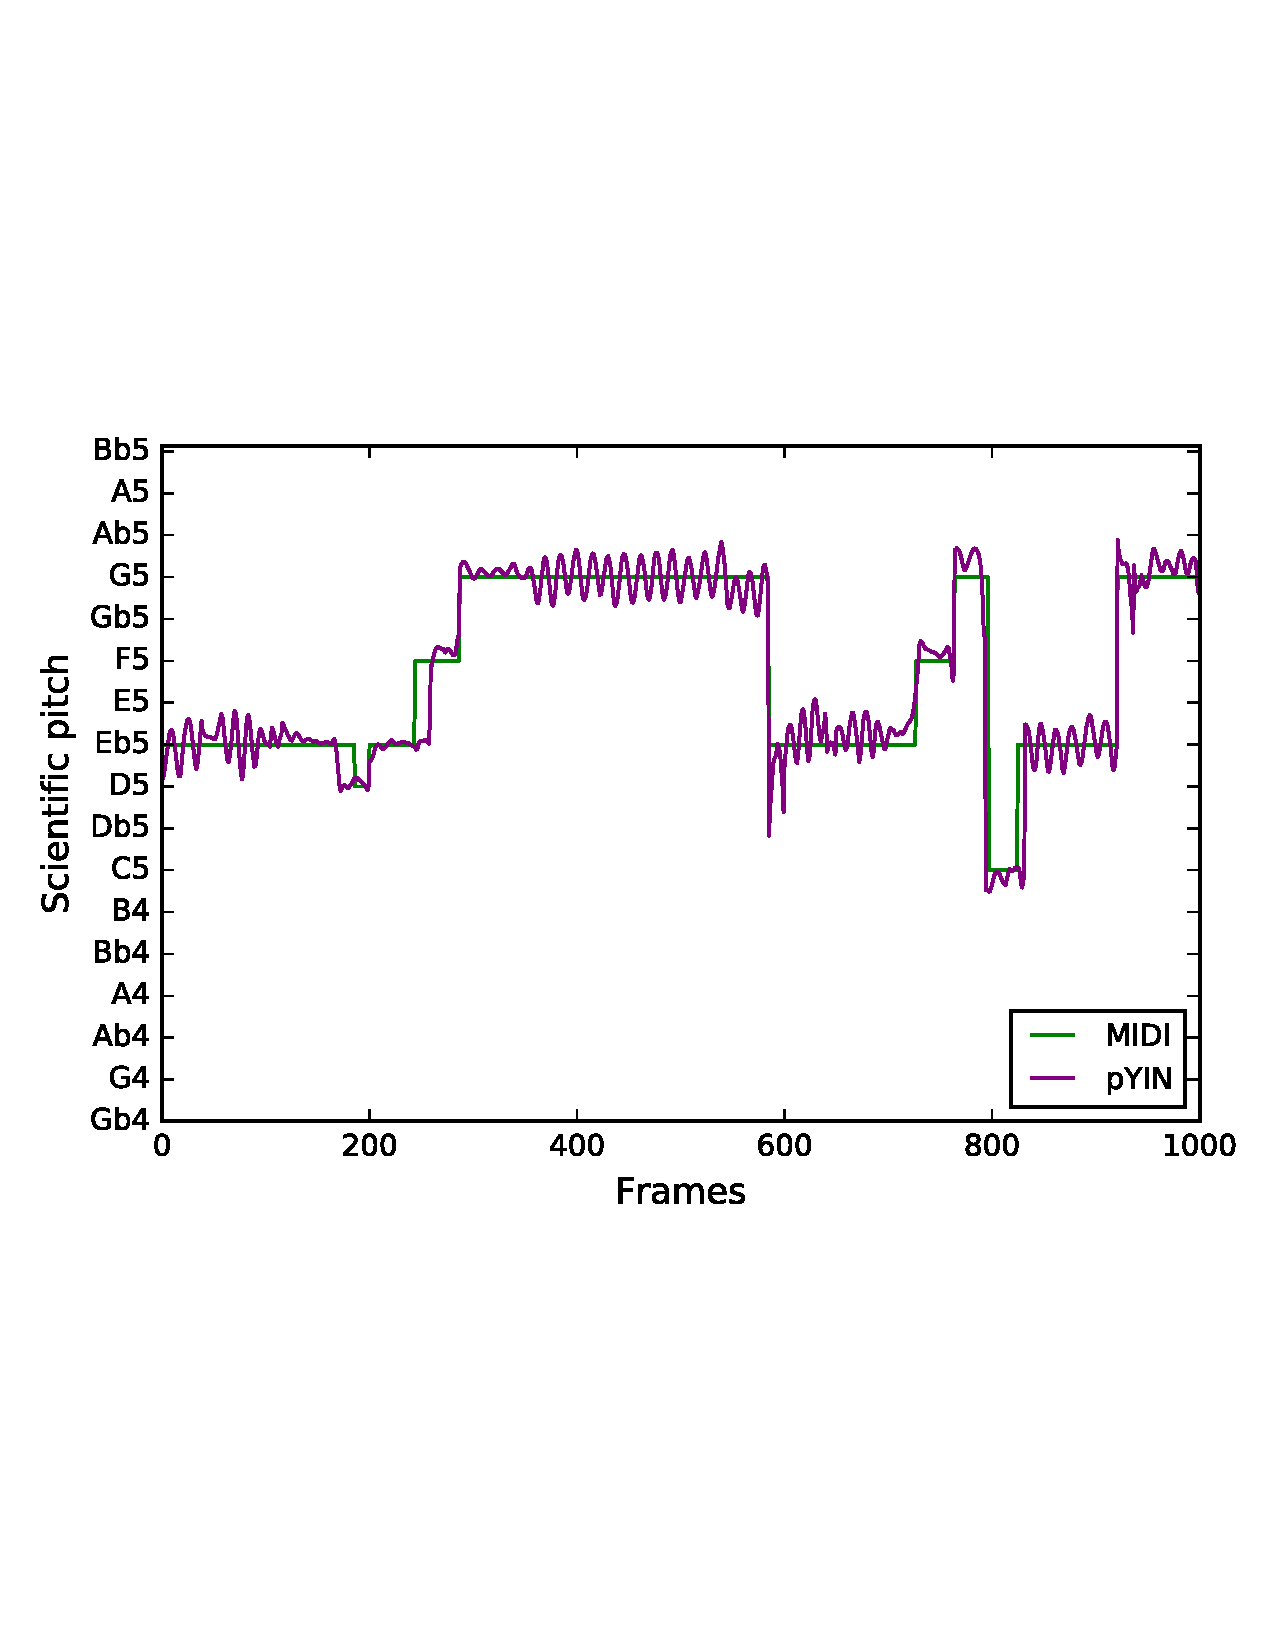
\includegraphics[width=0.5\textwidth]{figures/intonation_midi_and_pyin_aligned_active_54932280_1996063255.pdf}}\vspace{-1in}
    \subfigure{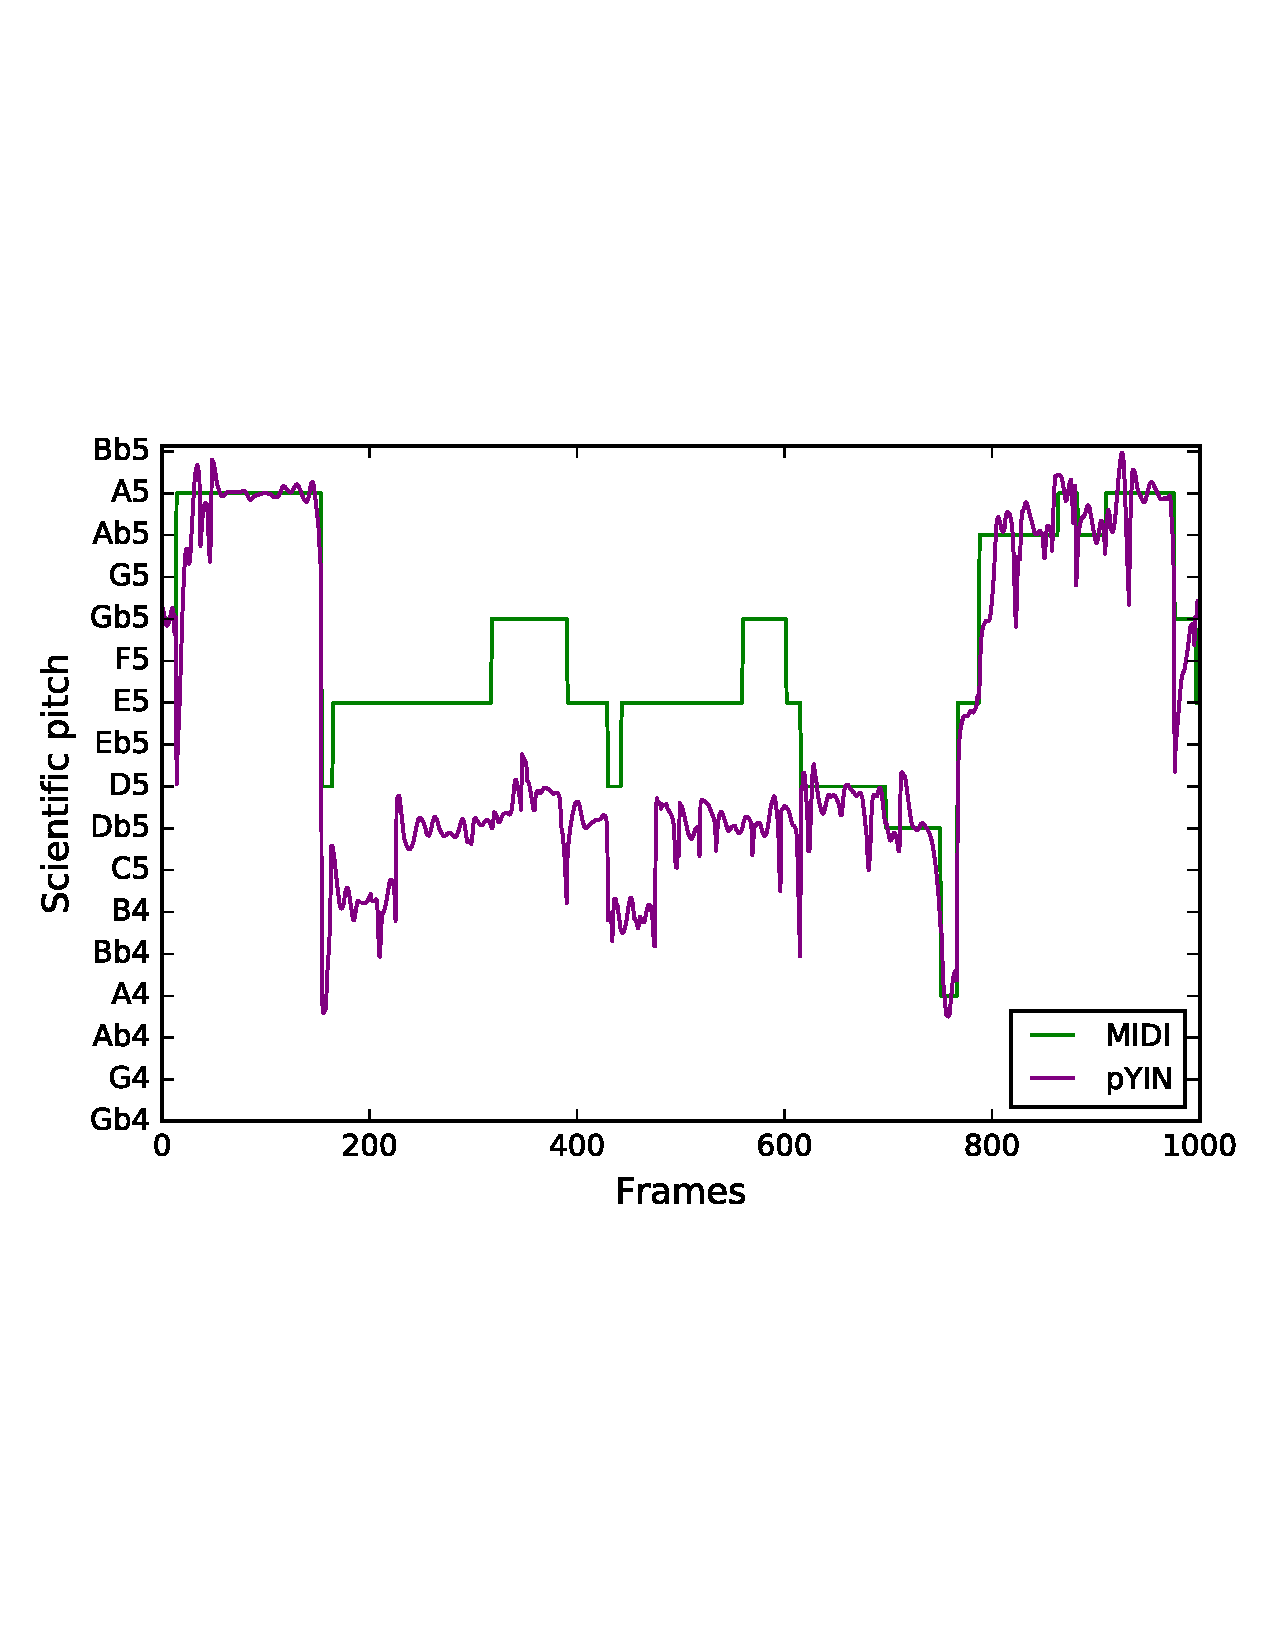
\includegraphics[width=0.5\textwidth, ]{figures/intonation_midi_and_pyin_aligned_active_544169967_2234781750.pdf}}\vspace{-1in}
    \subfigure{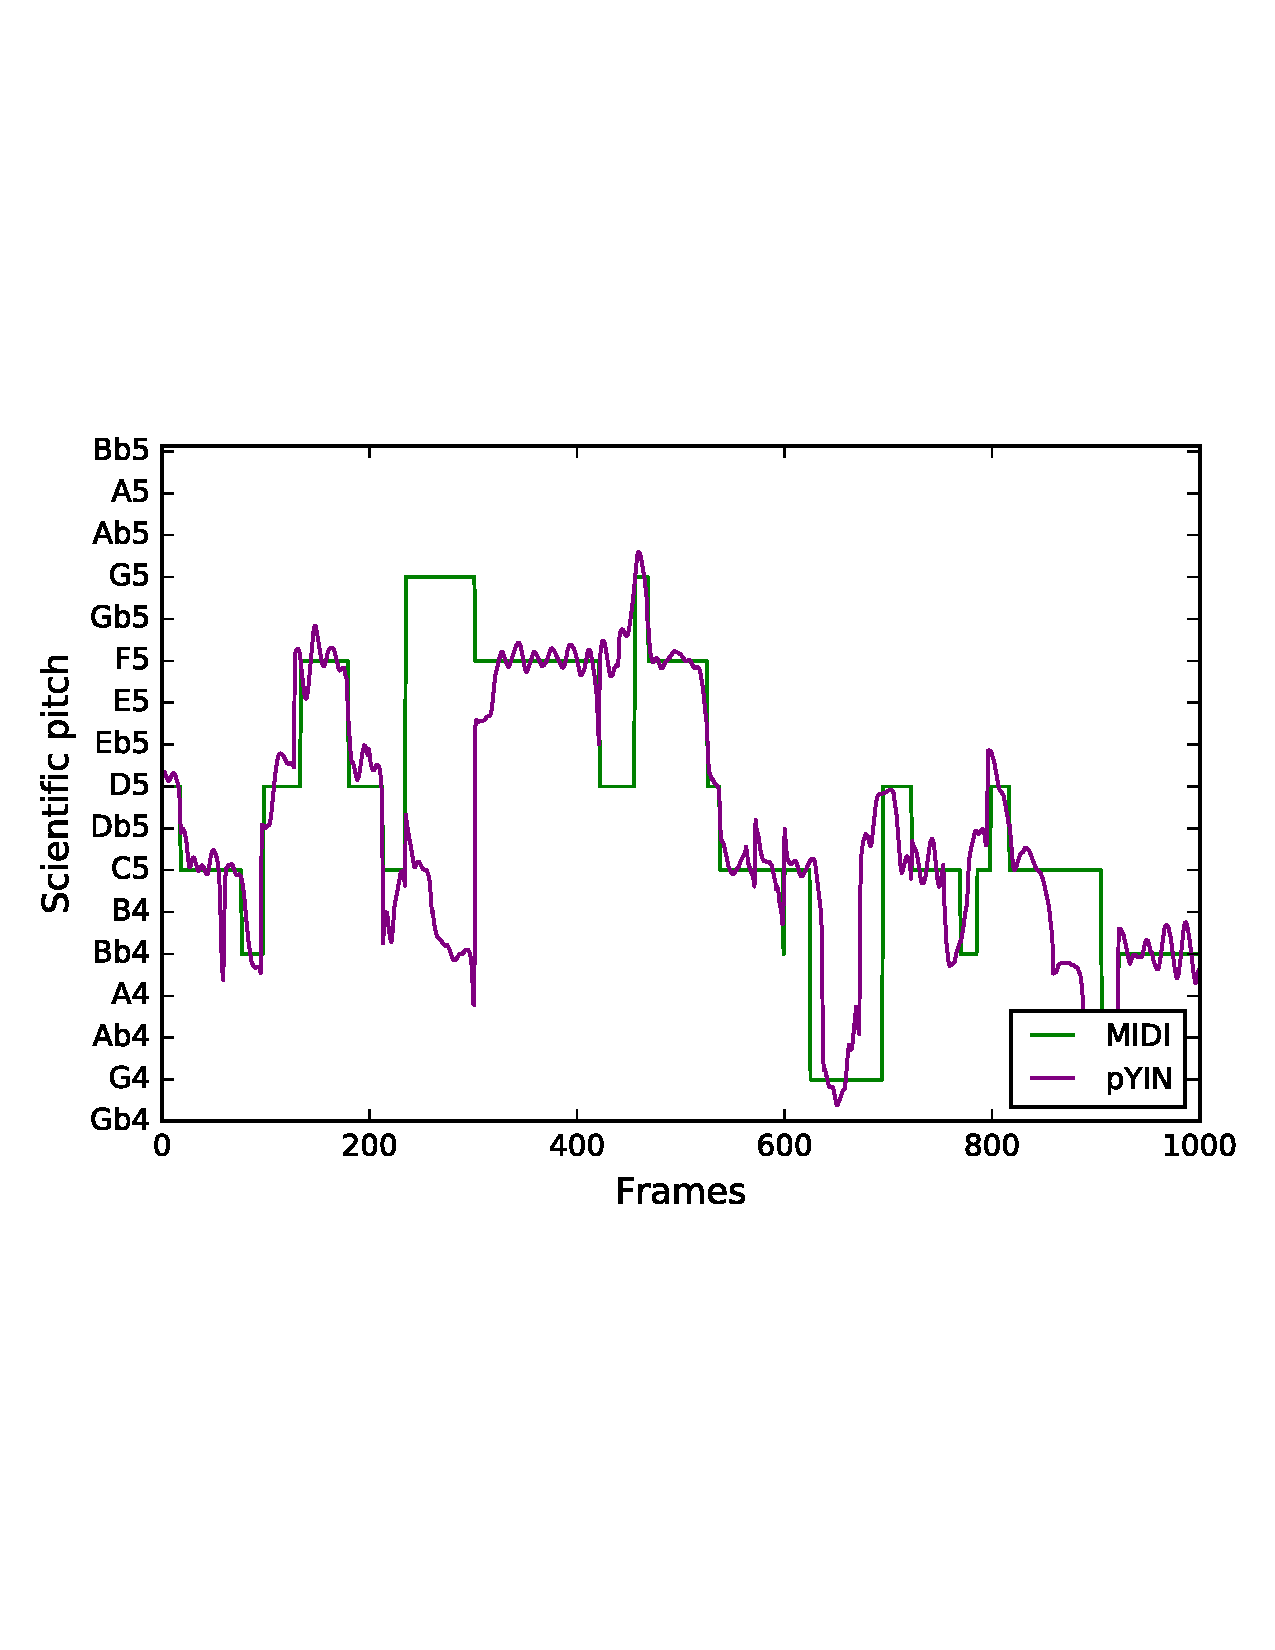
\includegraphics[width=0.5\textwidth, ]{figures/clustering_midi_and_pyin_aligned_active_545284262_2000375574.pdf}}\vspace{-0.5in}
    \subfigure{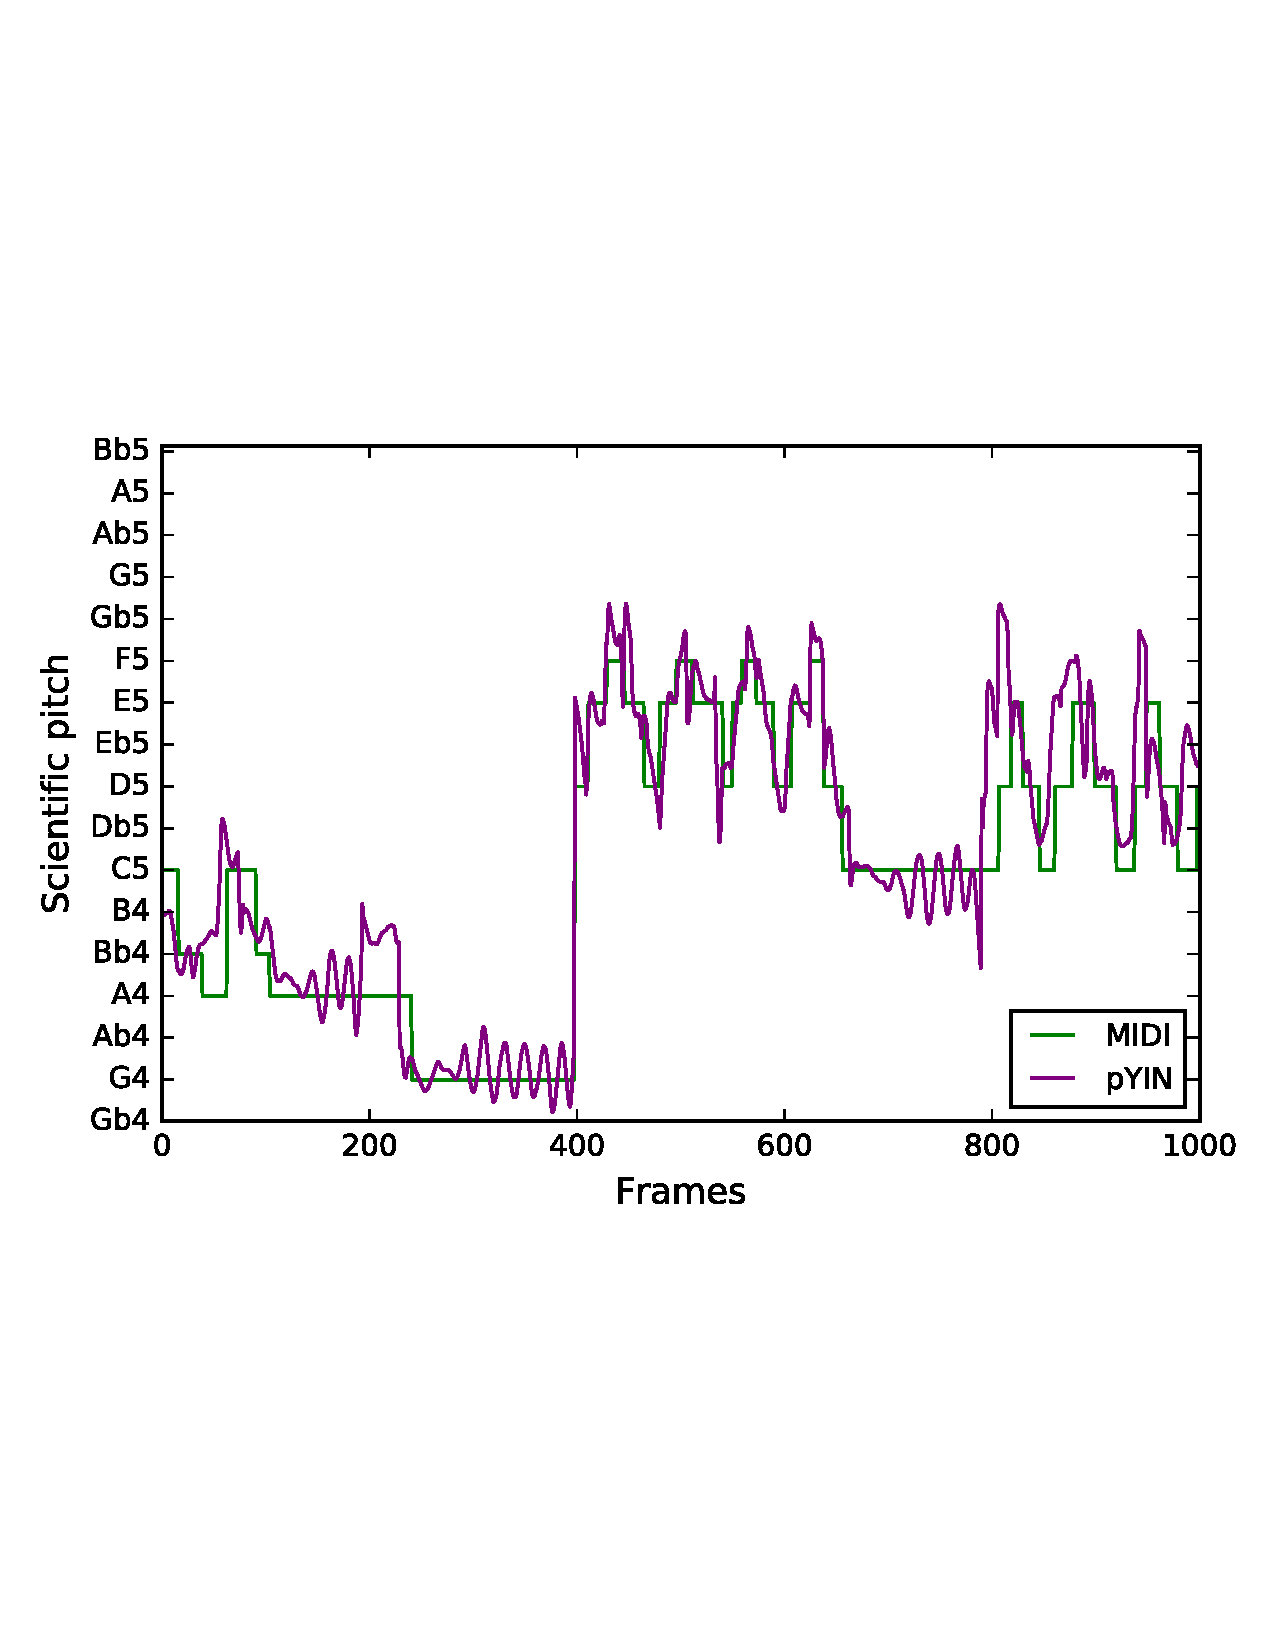
\includegraphics[width=0.5\textwidth, ]{figures/clustering_midi_and_pyin_aligned_active_54195986_1647186097.pdf}}\vspace{-0.5in}
    \caption{Singing pitch analysis of sample performances with aligned \gls{midi}. Two are in the clusters selected for  ``Intonation'' dataset (top), two in the remaining clusters (bottom). Much can be learned about the individual performances. The top two appear more tightly aligned to the expected pitch, though the second plot contains harmonization at a major third below the musical score. The vibrato in the first plot is particularly smooth, a sign of an advanced singer. The third plot shows frequent deviation from the score, while the fourth shows deviation at the beginning and the end but accuracy in the middle, along with a smooth vibrato. Still, it is difficult visually determine from this data format whether a performance sounds in tune.}
    \label{fig:sample_intonation}
\end{figure*}

%Related work
%- pitch deviation analysis
\section{Related work}
\label{sec:related}

\begin{figure}[h!]
    \centering
    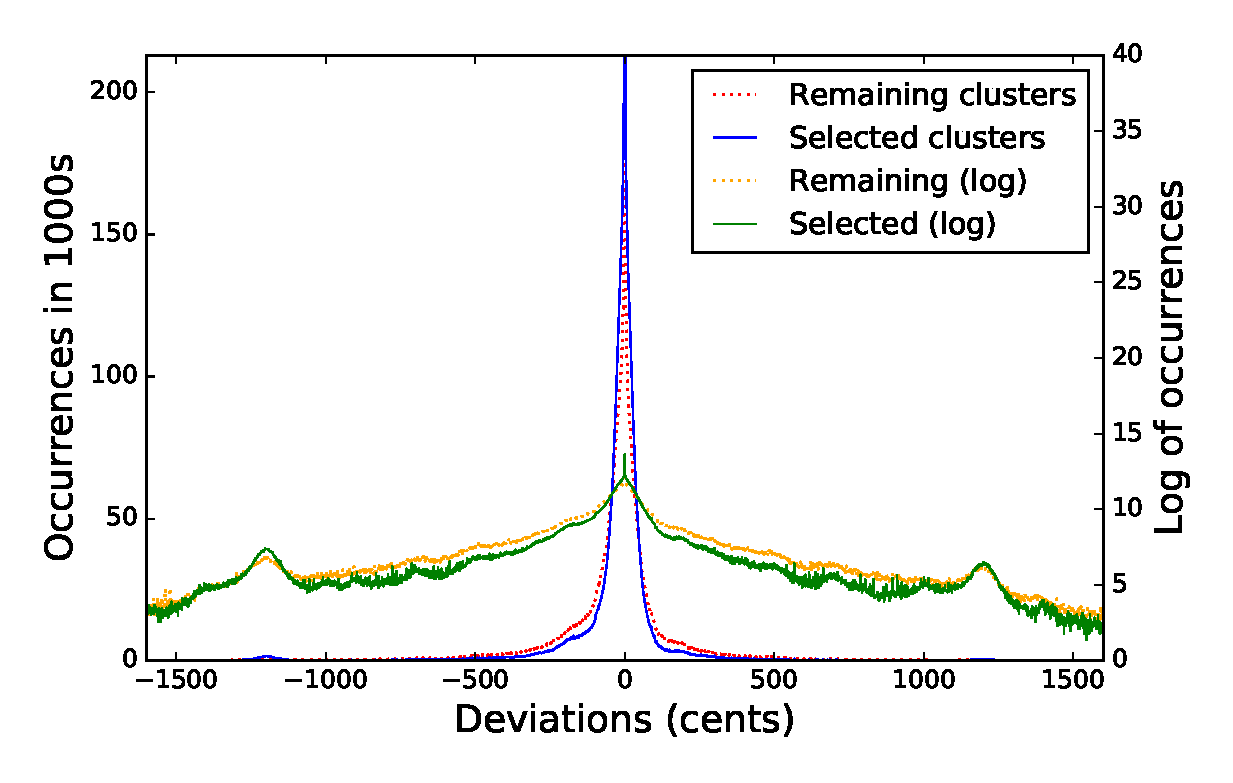
\includegraphics[width=\textwidth]{figures/full_histograms_comparison.eps}
    \caption{Global histograms of singing pitch deviations from the expected \gls{midi} pitch in cents summed over 4702 performances in the ``Intonation'' dataset and 4702 in the remaining clusters. The plot is truncated at the top for readability. Scaled log histograms make more noticeable the small peaks at 1200 cents in both directions, due to octave deviations, common among singers. There is also, interestingly, a larger number of deviations between 100 and 300 cents in the negative direction than in the positive direction.}
    \label{fig:full_hist}
\end{figure}

\subsection{Automatic pitch deviation analysis}
Automatic analysis of musical intonation behavior has also been performed in other contexts. For example, Nichols \textit{et al.} \cite{nichols2012automatically} described an approach to discovering talented singers on YouTube based on features extracted mostly from the audio. One of the main features they chose consisted of a pitch deviation histogram, which characterizes intonation behavior of a full performance in a low dimension. Given that the performances were typically not associated with a musical score and that the singing was mixed with the accompaniment and other background sounds, the authors built the histogram from the \gls{stft} amplitude peaks. A singer who sings flat should have a histogram skewed to the left, and an active vibrato will cause values to spread. The proposed feature extraction task is different from \cite{nichols2012automatically} because, as described below, the proposed model has access to the musical scores of the vocals and because the audio sources are separated. One can, therefore, apply a standard pitch detection algorithm to each vocal track and compare the results to the musical score. Comparison of performance pitch and musical score is also used by \cite{lim2010intune} in the context of a tool for musical performance visualization.


\begin{figure}[h!]
    \centering
    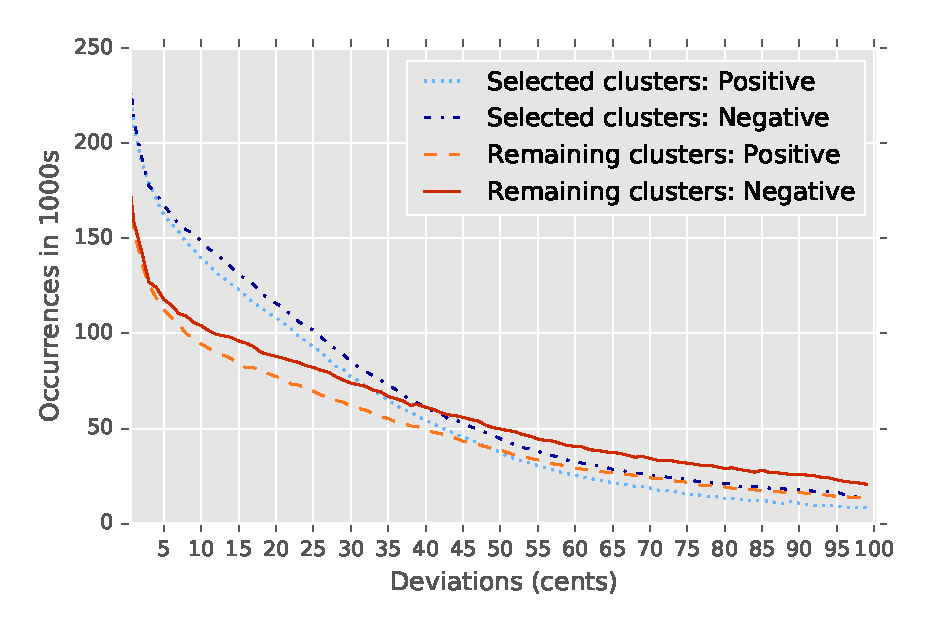
\includegraphics[width=\textwidth]{figures/full_pos_vs_neg_line.eps}
    \caption{Comparison of positive and negative deviation counts for cents ranging from 1 to 100 (omitting 0) for both datasets. In both groups, negative deviations are more common than positive ones. The ``Intonation'' dataset deviations are more concentrated around zero. }
    \label{fig:pos_neg}
\end{figure}

%Data collection and feature extraction
\section{Data collection and feature extraction}
\label{sec:features}
We collected solo vocal tracks of karaoke performances from a very large database. The first step was to filter for performances where singers used a headset---avoiding incorporating noise from the backing track into the recording. Given that we had access to a musical \gls{midi} score of expected pitches, we also used a simple heuristic to filter for performances that were aligned enough with the score to exclude scenarios such as people speaking instead of singing. We kept this heuristic lenient enough that in-tune performances where the singer used harmonization (sang different pitches than the expected melody) or made other intentional deviations from the \gls{midi} track wouldn't be excluded. This pre-filtering provided 14403 performances. 

The next step was to summarize intonation patterns of a performance using a low-dimensional set of features. The procedure is shown in Figure \ref{fig:pipeline} for two example performances. We first compared the singing pitch to the expected pitch in the \gls{midi} score. We computed the singing pitch using the pYIN algorithm \cite{mauch2014pyin} on one minute of audio, starting at 30 seconds to avoid silence, with one sample (frame) per 11 milliseconds. pYIN has a high frequency resolution because it is based in the time domain and refines results using linear interpolation. Resolution is crucial for musical intonation, where a few cents difference can determine whether a pitch sounds in or out of tune. We shifted the \gls{midi} score by a global constant to the octave nearest to the singing pitch, which can differ based on gender, age, and vocal type. We then computed the frame-wise absolute values of the difference in cents $\left| 1200 * log_2 \frac{f_1 + \epsilon} {f_2 + \epsilon} \right|$ between the performance and \gls{midi} score. Of this set of values, we kept the differences less than or equal to 200 cents, equivalent to two semitones, in order to focus the analysis on intonation behavior when the singer was close to the expected pitch. Larger differences could be due to many reasons, ranging from misalignment of notes in time to harmonization, and might add undesired noise to the distributions. 

Finally, we summarized these variable-length sequences of frame-wise differences in a fixed, low-dimensional representation. We generated a random sample of 10,000 differences with replacement for every performance and kept 31 evenly spaced quantiles. This empirically chosen number is large enough to effectively summarize the characteristics of the distribution but produces a low enough dimensionality for clustering.

\begin{figure}[h!]
    \centering
    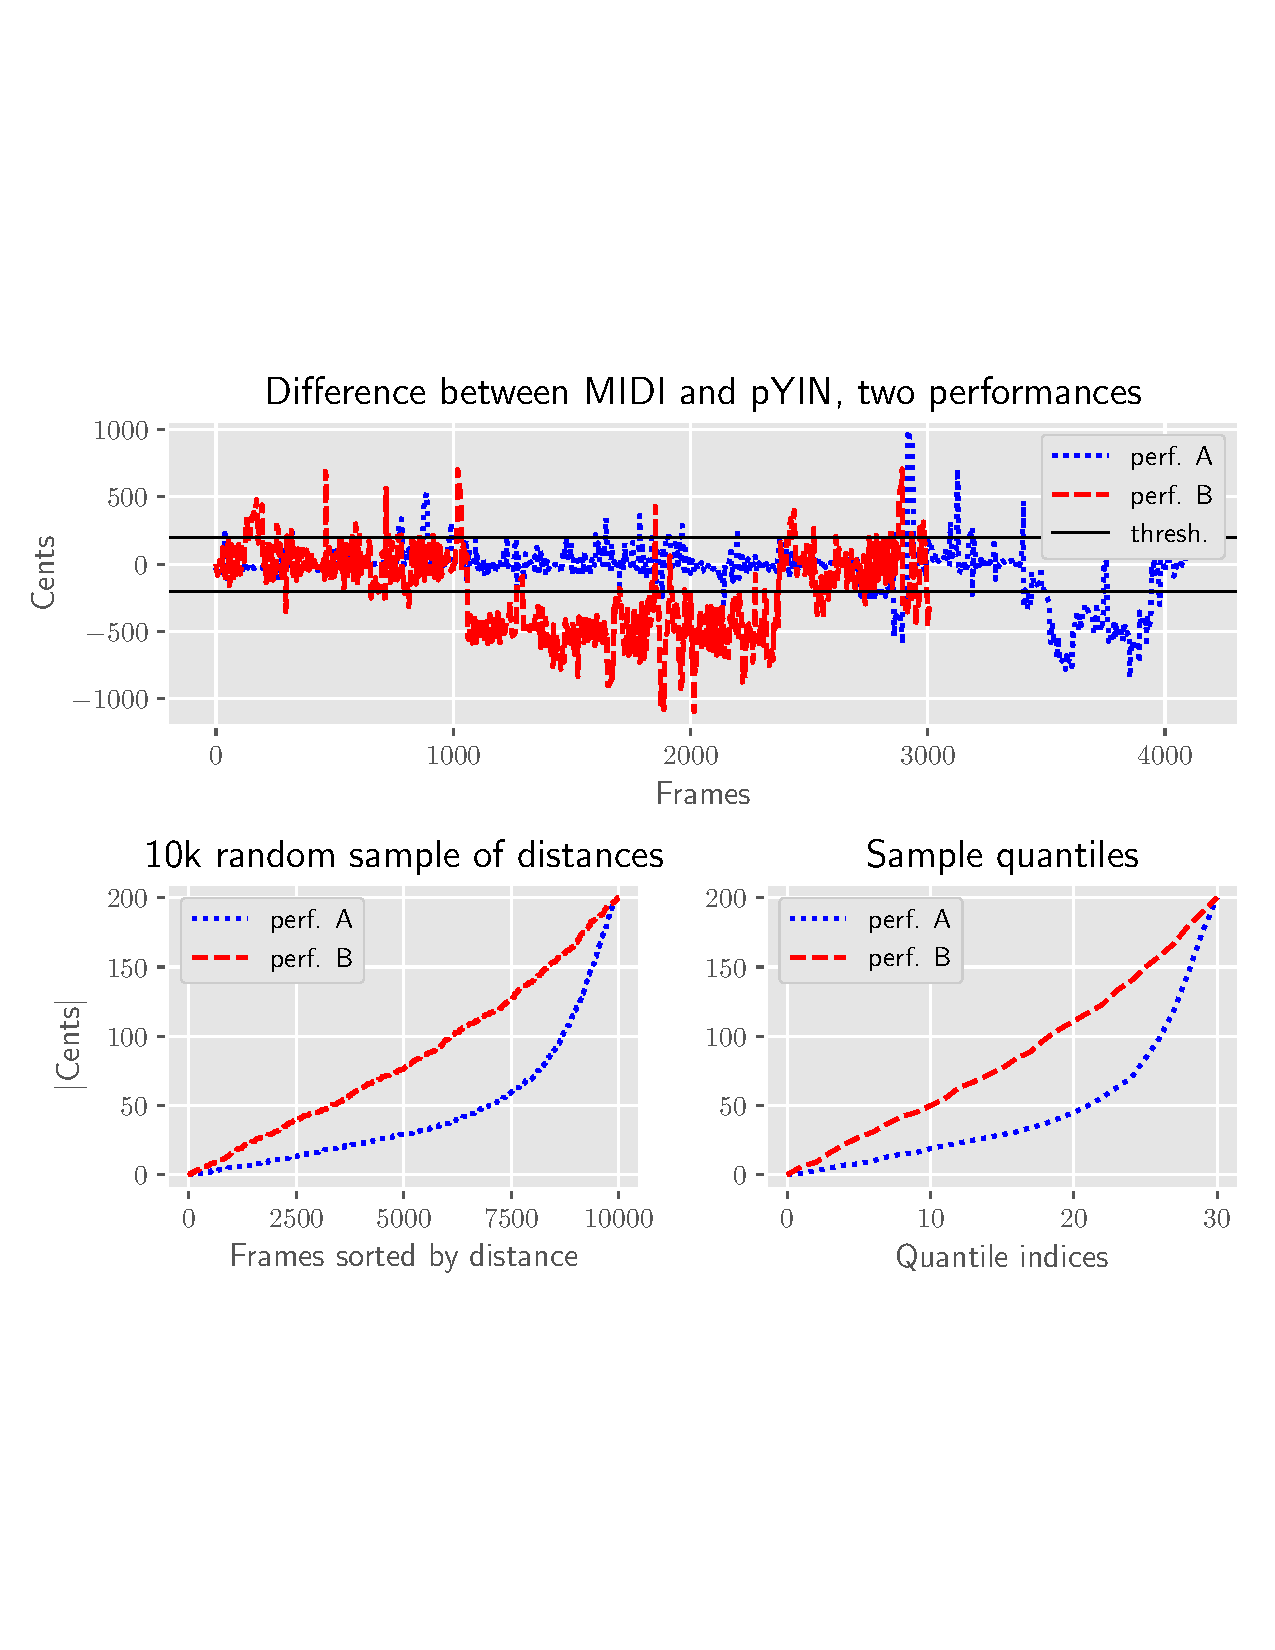
\includegraphics[width=\textwidth]{figures/data_processing_pipeline.pdf}\vspace{-1in}
    \caption{Data pre-processing steps for two example performances. The blue performance was selected for the ``Intonation'' dataset and the red performance was not. The first plot shows the frame-wise differences in cents between the measured singing pitch and equal-tempered \gls{midi} score. We computed the absolute values of these differences and discarded those whose deviation was larger than 200 cents. The second plot shows random samples of 10,000 from the frame-wise difference lists, sorted by distance. The blue curve shows less deviation from the expected pitch than the red. The third plot shows 31 quantiles summarizing the curve in the second plot in a lower dimension.}
    \label{fig:pipeline}
\end{figure}
%Spectral clustering
% - genres and bias
\section{Spectral clustering}
As suggested by the studies described in Chapter \ref{chap:intonation}, an advanced singer might produce both smaller and wider pitch deviations, due to a pronounced vibrato or expressive variations such as pitch bending, time shifting, or harmonization, than a singer who sings close to the musical score but is slightly off pitch. For this reason, selecting performances based on a simple metric like average distance of singing pitch from the score would not have been suitable. A semi-supervised approach also made it possible to avoid directly modeling the concept of being in tune. The approach clustered performances based on features generated from the deviations. The choice of which cluster to keep was based on listening to samples from each.

Spectral clustering was applied to the summarized performances using the signless Laplacian matrix as the adjacency graph \cite{lucinska2012spectral}. This graph is based on selecting nearest neighbors (50 in this case). In practice, the program clustered approximately 5000 songs at a time into 3 or 4 clusters, depending on which value produced better Newman modularity \cite{newman2006modularity}. I then listened to 50 samples from every cluster and subjectively determined the intonation of every performance by evaluating it as in tune, ``neutral'', out of tune. Consistently, one cluster produced distinctly good results with roughly 75 per cent of the songs classified as in tune and many of the remaining songs being classified as neutral rather than out of tune, while the other clusters had only a small percentage of performances classified as in tune. 

Keeping the samples from the selected clusters resulted in the ``Intonation'' dataset of 4703 performances. Though not every performance is in tune and not every performance in remaining clusters is out of tune, a majority of in-tune performances in this dataset suffices for many machine-learning applications.

\subsection{Genre, bias, and related challenges}
An undesirable outcome of this clustering approach was that musical genres were clustered along with intonation patterns. As described in Chapter \ref{chap:intonation}, different musical traditions and sub-traditions often have diverging traditions regarding musical intonation. In the Smule samples, a majority were of Western popular music, and the in-tune clusters tended to consist mostly of such music. I had planned to use performances from other clusters for testing, but realized that many of the performances were country, where singers deliberately might wish to sing flat, and the automatic pitch correction model trained on a different genre might not apply. As this was an intern project, I do not currently have the ability to update the clustering technique, and have to focus on the effects of the proposed algorithm on Western pop music. In future work, if implementing this program for real-world use, I would first separate performances by genre, then apply spectral clustering within the genre. This improvement requires advanced genre classification, but this field is growing and improving quickly in the context of music recommendation systems.  

%Analysis
\section{Analysis}

The quality of the dataset is difficult to measure without a subjective listening test. At this point, we do not attempt to directly show that the ``Intonation'' dataset performances have better intonation than those in the remaining clusters. Instead, we show a difference in the intonation behavior distributions in the two collections. In order to compare samples of the same size, we analyzed the full ``Intonation'' dataset of size 4702 and a randomly selected a sample of the same size of performances from the remaining clusters.

\subsection{Data pre-processing for analysis}
We computed the frame-wise differences between singing pitch and \gls{midi} score similarly to the way described in Section \ref{sec:features}. Unlike before, we retained the sign instead of taking the absolute value in order to know whether the pitch was sharp or flat. We also kept all deviations instead of discarding those larger than 200 cents: At the analysis stage, we are interested in intonation characteristics across the whole performance, including the larger deviations due to harmonization, expressive deviations, or inaccuracy. 

To minimize misalignment before computing the deviations, we applied dynamic time warping \cite{berndt1994using} to better align the \gls{midi} and singing pitch tracks. This algorithm stretches both signals in time in a way that minimizes the total sum of distances between the two. We used the algorithm as described in \cite{muller2015fundamentals} and implemented in \cite{mcfee2015librosa}. To avoid distorting the pitch track, we forced the algorithm to apply most time warping to the \gls{midi}, which consists of straight lines. We discarded frames where either the musical score or pitch tracks were silent in order to only consider active frames in the analysis. Figure \ref{fig:sample_intonation} shows four example performances after the initial processing. The top two are from the selected clusters and the bottom two from the remaining clusters.

\subsection{Pitch deviation histogram}
We compared the sequences of frame-wise pitch deviations from the selected clusters to those from the remaining clusters. Similarly to \cite{nichols2012automatically}, we computed histograms of the deviations from the equal-tempered \gls{midi} score summed over all performances in each group, normalizing them to have the same total counts. Figure \ref{fig:full_hist} shows that the ``Intonation'' dataset deviations are more concentrated very close to 0 than those in the remaining clusters. The same can be observed at other harmonization peaks, $\pm1200$ cents (an octave) and other values in between, indicating more intentional harmonization and less accidental deviation. There is also, interestingly, a higher concentration of counts between 100 and 300 cents especially in the negative direction. This dataset is of amateur singing, so there is also a chance that some singers would be singing flat. However, this clearly visible peak might be due to intentional harmonization and expressive suspensions. 

\subsection{Pitch deviation probabilities}
We examined whether we could find intonation tendencies like those described in Section \ref{sec:empirical}. Unlike in the data used in the cited studies, the backing tracks are fixed recordings, so all pitch adjustments happen in the voice. This can affect the pitch deviation distributions. In Figure \ref{fig:pos_neg}, we examine deviations within 100 cents because a larger deviation corresponds a different note. Both collections tend towards negative deviations, but the tail is lighter in the selected clusters.

We quantify this result by estimating the probability of negative versus positive deviations within various absolute deviation thresholds using bootstrapping \cite{efron1994introduction} with 10000 iterations, as shown in Table \ref{table:1}. We choose ranges of cents that are of interest when comparing theoretical musical intervals generated using the equal temperament versus other intonation systems (e.g., Pythagorean or Just intonation, described in the cited studies). Use of other intonation systems would explain deviations of 2 to 16 cents. We first examine the ratio of deviations less than 2 cents. As expected, a probability of 0.5 shows no significant preference for flat versus sharp intonation. Within 2 to 16 cents, we get 0.51. However, the largest probabilities occur at larger values, 300 cents. We cannot determine whether this deviation is a desirable effect or due to an unknown factor. The tendencies are observed in both collections. 


\begin{table}[t!]
\centering
\begin{tabular}{ |c|c|c| } 
\hline
\multicolumn{3}{|c|}{Results from ``Intonation'' dataset (4702 performances)}\\
\hline\hline
Cents range & Negative/positive deviation ratio & Var \\
\hline
1 to 2 & 0.500 & 0.001 \\ 
2 to 16 & 0.506 & 0.001 \\ 
1 to 100 & 0.532 & 0.002\\ 
100 to 300 & 0.727 & 0.002\\ 
\hline\hline
\multicolumn{3}{|c|}{Results from other performances (9701 performances)}\\
\hline\hline
Cents range & Negative/positive deviation ratio & Var \\
\hline
1 to 2 & 0.500 & 0.001 \\ 
2 to 16 & 0.509 & 0.001 \\ 
1 to 100 & 0.541 & 0.002\\ 
100 to 300 & 0.700 & 0.002\\ 
\hline
\end{tabular}
\caption{Probability estimates of negative versus positive frame-wise deviations of singing pitch from the equal-tempered \gls{midi} score, computed using bootstrapping. The analysis was performed within different ranges of interest. When the deviation is less than 100 cents, the singer did not sing a different note. We found a particularly strong tendency towards negative deviations in the range of 100 to 300 cents.}
\label{table:1}
\end{table}

%Dataset description and applications
\section{Dataset description and applications}
The ``Intonation'' dataset contains the full unmixed and unprocessed vocal tracks of 4702 performances. It consists of 474 unique arrangements by 3556 singers. It also contains the \gls{pyin} pitch analysis and multiple backing track features for the range of 30 to 90 seconds: constant-Q transform, chroma, mel-frequency cepstrum coefficients, root mean square error, and onset, all computed using the Librosa \cite{mcfee2015librosa} package. Metadata of the performances is included. The dataset has applications ranging from the study of singing style in the context of karaoke performances, with optional study of user meta-data, to machine learning. For example, the vocal tracks can be used for informed source separation, an approach similar to separation by humming, described in \cite{smaragdis2009separation} and \cite{liutkus2012informed}. Similarly, the dataset can be used for training a query-by-humming system, in a similar way to \cite{huq2010crowdsourcing}. The vocal pitch tracks and backing track features can be used to study automatic pitch correction applications trained on real-world singing and develop a proof-of-concept model for vocal pitch correction \cite{wager2018pitch}.

%Conclusion
\section{Summary}
We present a semi-automatic process for the task of searching through a large database of amateur karaoke performances for samples with a tendency for good musical intonation. The approach can be applied in other situations where a researcher needs to extract a subset of data samples from a large database. We show that the set of collected performances has a different intonation behavior distribution than the set of remaining performances. The resulting public dataset, ``Intonation'', of 4702 performances is available on the Stanford CCRMA DAMP website. The ``Intonation'' dataset can be used for music information retrieval applications like query-by-humming systems. Analyzing the dataset, we find that pitch deviations between the measured singing pitch and the \gls{midi} score are more often negative than positive, implying that singers more often choose lower frequencies, use them unintentionally by singing flat, or decorate pitch contours with flat sections.

%%%%%%%%%%%%%%%%
% Chapter 6
%%%%%%%%%%%%%%%%

\chapter{Conclusion}
Lorem ipsum dolor sit amet, consectetur adipiscing elit, sed do eiusmod tempor incididunt ut labore et dolore magna aliqua. Ut enim ad minim veniam, quis nostrud exercitation ullamco laboris nisi ut aliquip ex ea commodo consequat. Duis aute irure dolor in reprehenderit in voluptate velit esse cillum dolore eu fugiat nulla pariatur. Excepteur sint occaecat cupidatat non proident, sunt in culpa qui officia deserunt mollit anim id est laborum.


%%%%%%%%%%%%%%%%
% Chapter 7
%%%%%%%%%%%%%%%%

%\chapter{Conclusion}
Lorem ipsum dolor sit amet, consectetur adipiscing elit, sed do eiusmod tempor incididunt ut labore et dolore magna aliqua. Ut enim ad minim veniam, quis nostrud exercitation ullamco laboris nisi ut aliquip ex ea commodo consequat. Duis aute irure dolor in reprehenderit in voluptate velit esse cillum dolore eu fugiat nulla pariatur. Excepteur sint occaecat cupidatat non proident, sunt in culpa qui officia deserunt mollit anim id est laborum.


%%%%%%%%%%%%%%%%
% Appendices
%%%%%%%%%%%%%%%%

\begin{appendices}

%Some Table of Contents entry formatting
\addtocontents{toc}{\protect\renewcommand{\protect\cftchappresnum}{\appendixname\space}}
\addtocontents{toc}{\protect\renewcommand{\protect\cftchapnumwidth}{6em}}

%Begin individual appendices, separated as chapters

\chapter{``Intonation'': A dataset of quality vocal performances refined by spectral clustering on pitch congruence}
\label{chap:thesis-damp}
%Introduction
%- dataset of musical performances
%    - how to gain access
\section{Overview and access}
This chapter describes the set of vocal performances used to train the autotuning program, and how I collected it.\footnote{This work was supported by the internship program at Smule, Inc.} The ``Intonation'' dataset consists of amateur vocal performances with a tendency for good intonation, collected from Smule, Inc. The dataset can be used for music information retrieval tasks such as autotuning, query by humming, and singing style analysis. It is publicly available.\footnote{The dataset and detailed description of the contents are available upon request via \url{https://ccrma.stanford.edu/damp}.} We describe a semi-supervised approach to selecting the audio recordings from a larger collection of performances based on intonation patterns. The approach can be applied in other situations where a researcher needs to extract a subset of data samples from a large database. A comparison of the ``Intonation'' dataset and the remaining collection of performances shows that the two have different intonation behavior distributions. 

%- semi-supervised approach that can be used for other data %collection tasks (describe in next section)
%- provides an analysis in light of chapter 2
Pitch in a karaoke context and, more generally, in many scenarios where a musical score is used, is modeled as the twelve discrete frequencies per octave, evenly spaced in the logarithmic scale, that constitute the equal-tempered scale. Quantitative and qualitative studies on musical intonation of professional-level singers, however, indicate frequent, deliberate deviations from the equal-tempered scale. In particular, musicians often sing or play sharp relative to an accompaniment. \cite{parncutt2018psychocultural} describes this phenomenon, citing \cite{barbour1938just, schoen1926pitch, cameron1907tonal}. Research such as described in \cite{devaney2011intonation} finds much variety in musical interval sizes both above and below the equal-tempered intervals in polyphonic choral music. The results are interesting in our context because they indicate that the pitch of good singers might not simply deviate from a center pitch that is equal to the equal-tempered pitch we will find in a musical score. Instead, singers may choose to center their pitch at a different frequency. In this paper, we analyze the ``Intonation'' dataset to check whether its amateur performances of mostly Western popular music show similar tendencies to those described in the studies.

%Need for music datasets
%- semi-supervised approach
section{Music datasets and related work}
Useful datasets have been made available for certain research topics in the fields of music information retrieval and audio. These include sound event detection \cite{Mesaros2018_DCASE}, source separation \cite{SiSEC17}, and recommendations \cite{bertin2011million}. Sometimes, though, the best dataset available for a topic is huge and difficult to process. A large collection of audio recordings is available, but the recordings with suitable characteristics for the given analysis form a smaller subset of the dataset. The filtering process to extract the desired samples can be labor intensive, requiring that the researcher select the samples with the desired features, which may or may not be labeled and can be hard to model. One way to approach this selection process is to automate it using feature engineering and clustering. 

In this paper, we present this kind of semi-automatic process for the task of searching through a large database of amateur karaoke performances for samples with a tendency for good musical intonation. The need for this task arose when we wished to train a machine-learning model to predict pitch correction. We needed to select performances that were in tune enough but not those that were out of tune or contained little singing. We note that this task requires quantifying the concept of singing ``in tune''. As we describe in further sections, the task is not obvious, so we avoid creating an explicit definition of ``in tune'' by using a semi-supervised approach. We first extract musical intonation features from each performance, then apply spectral clustering to them and subjectively choose clusters that sound ``in tune'' by listening to samples from each. We also introduce the resulting dataset and an analysis of the intonation tendencies of its performances. Though we present this approach for our specific task, it can be adapted to other tasks, datasets, and features.

\begin{figure*}[h!]
    \subfigure{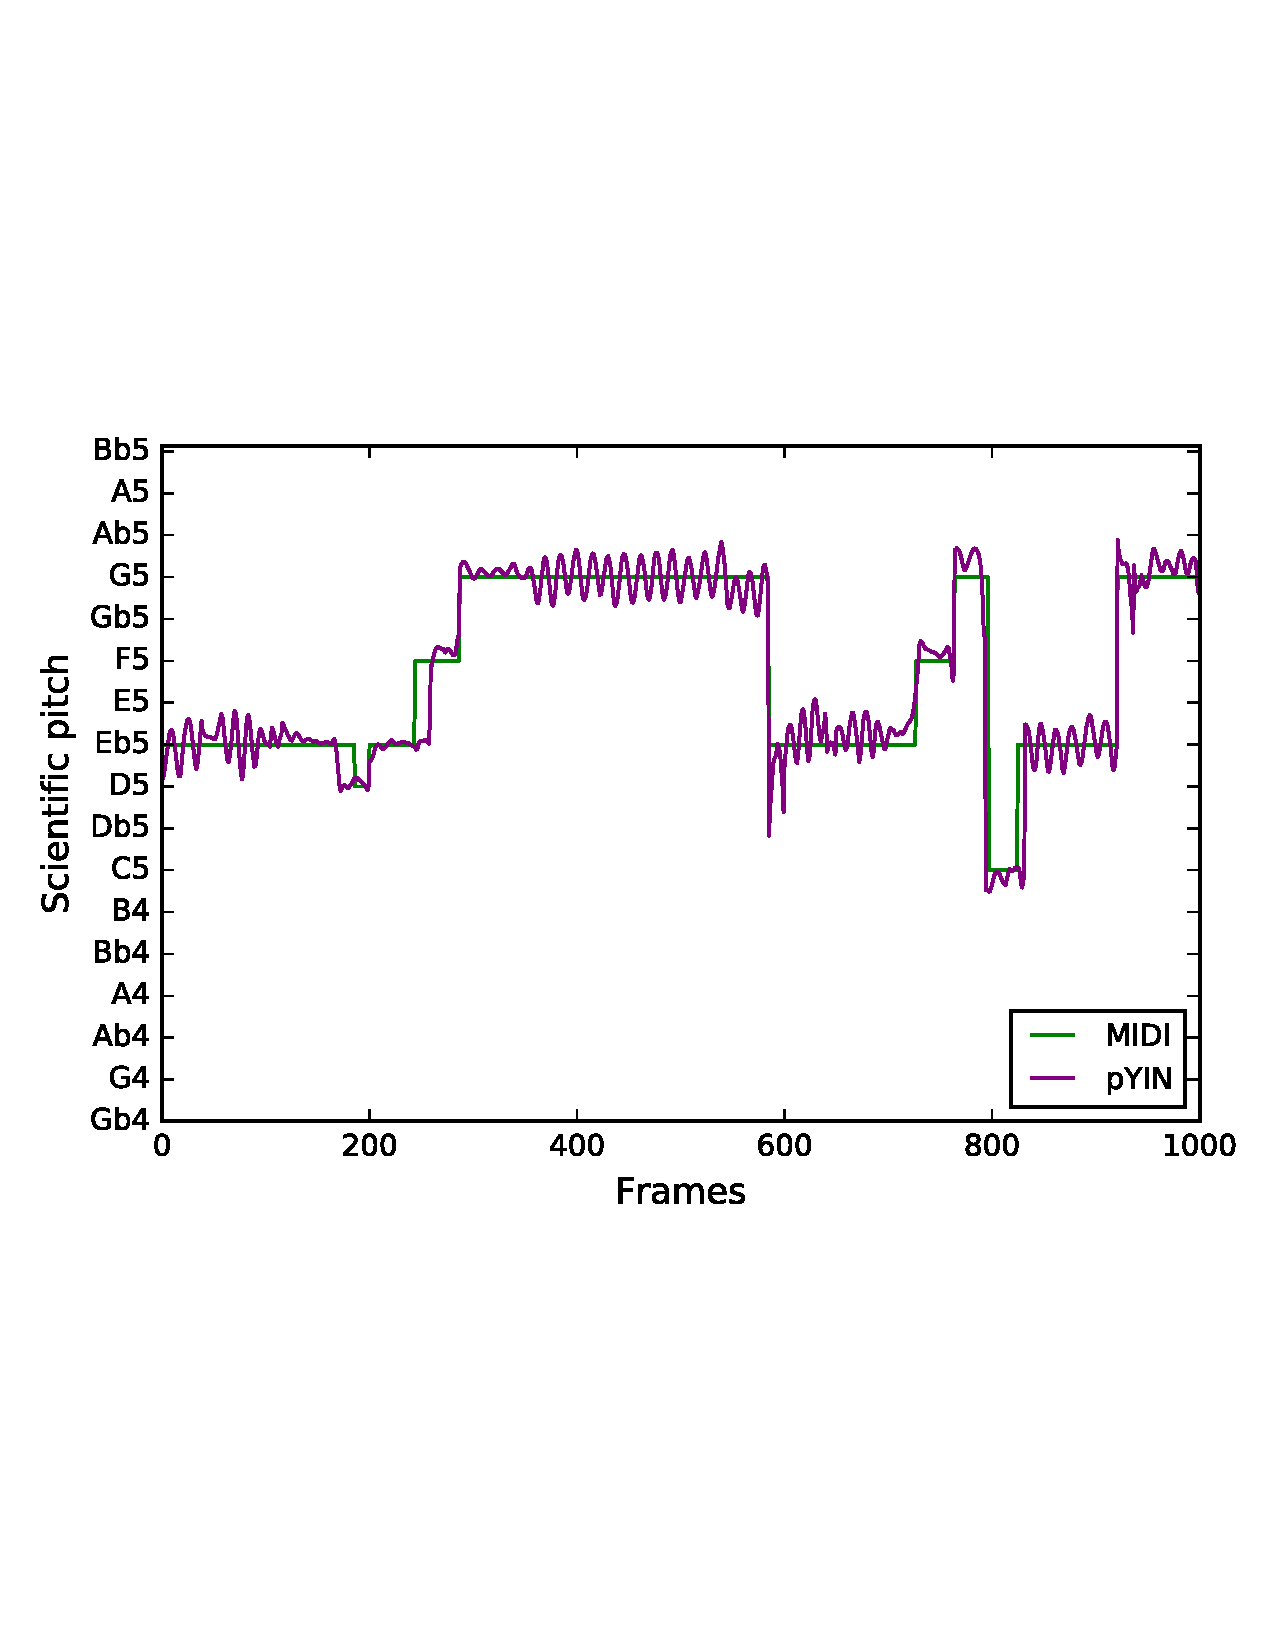
\includegraphics[width=0.5\textwidth]{figures/intonation_midi_and_pyin_aligned_active_54932280_1996063255.pdf}}\vspace{-1in}
    \subfigure{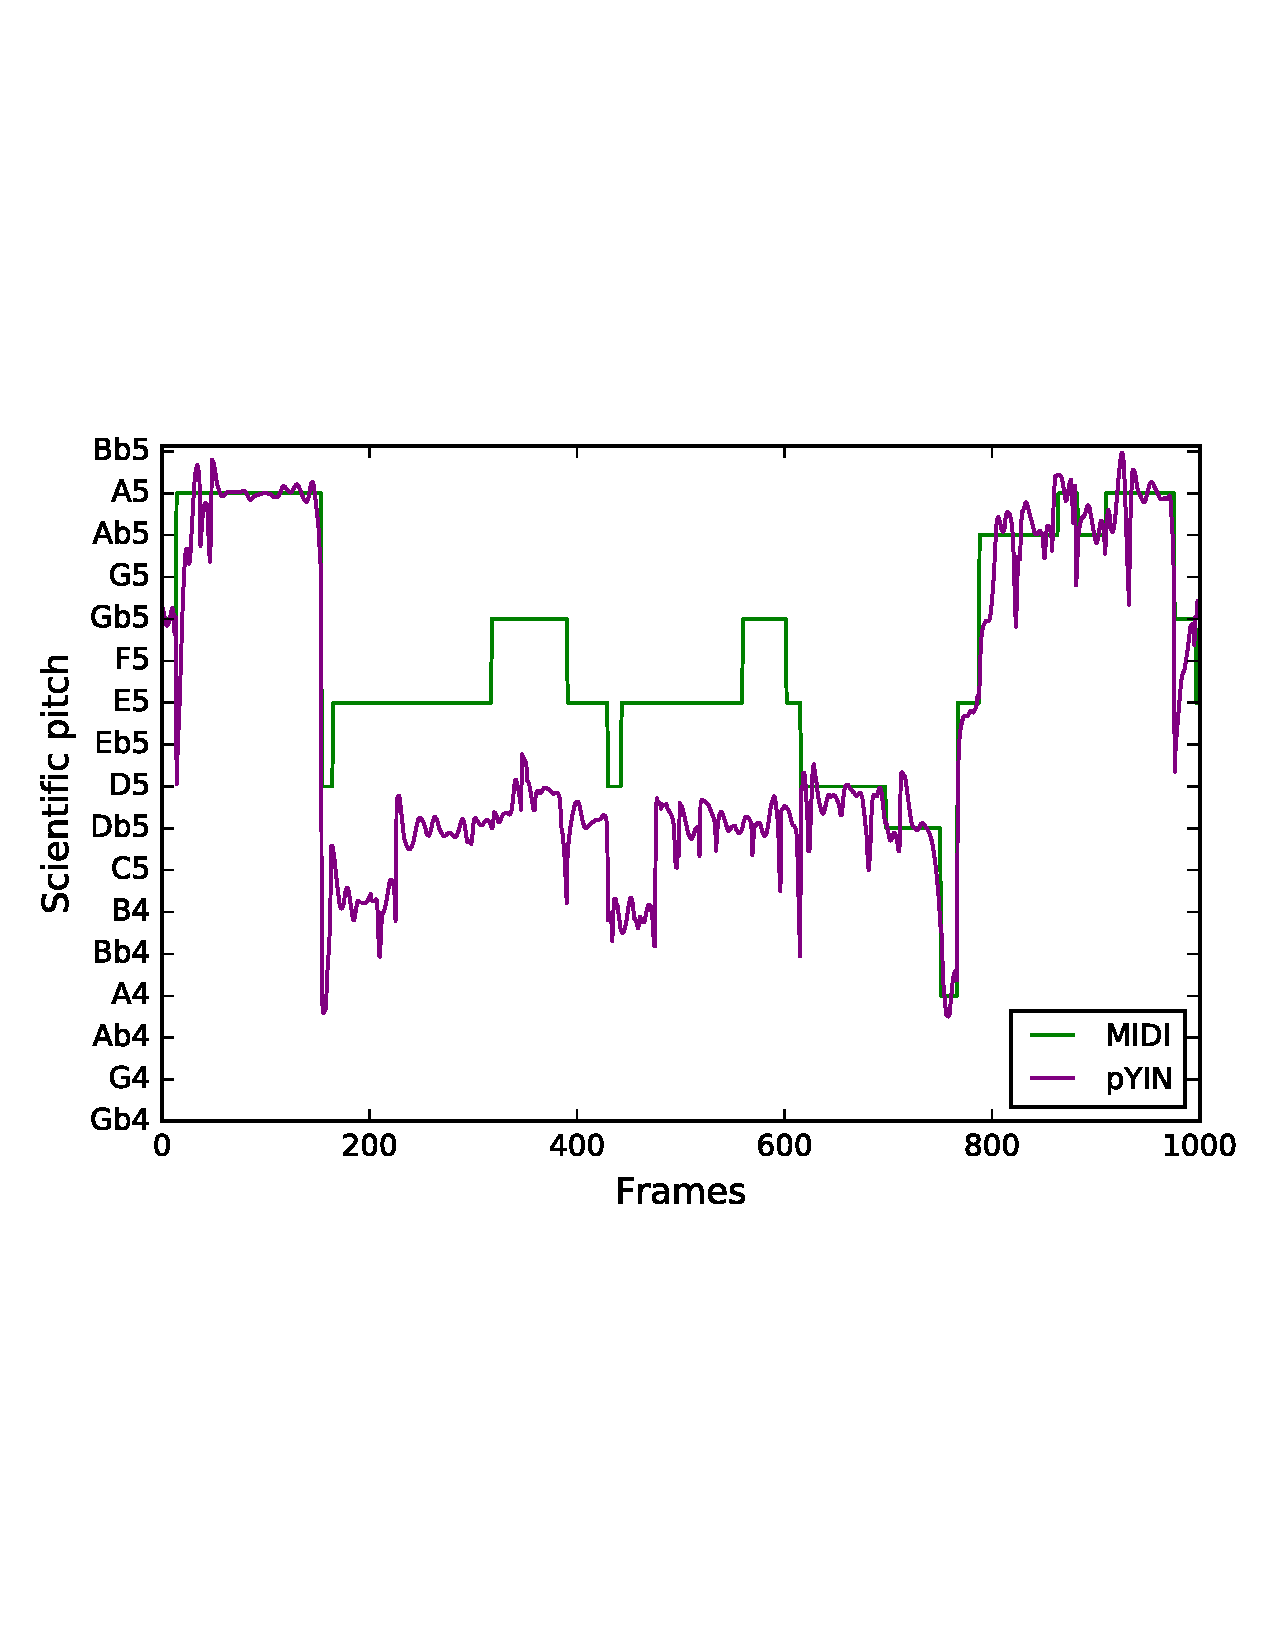
\includegraphics[width=0.5\textwidth, ]{figures/intonation_midi_and_pyin_aligned_active_544169967_2234781750.pdf}}\vspace{-1in}
    \subfigure{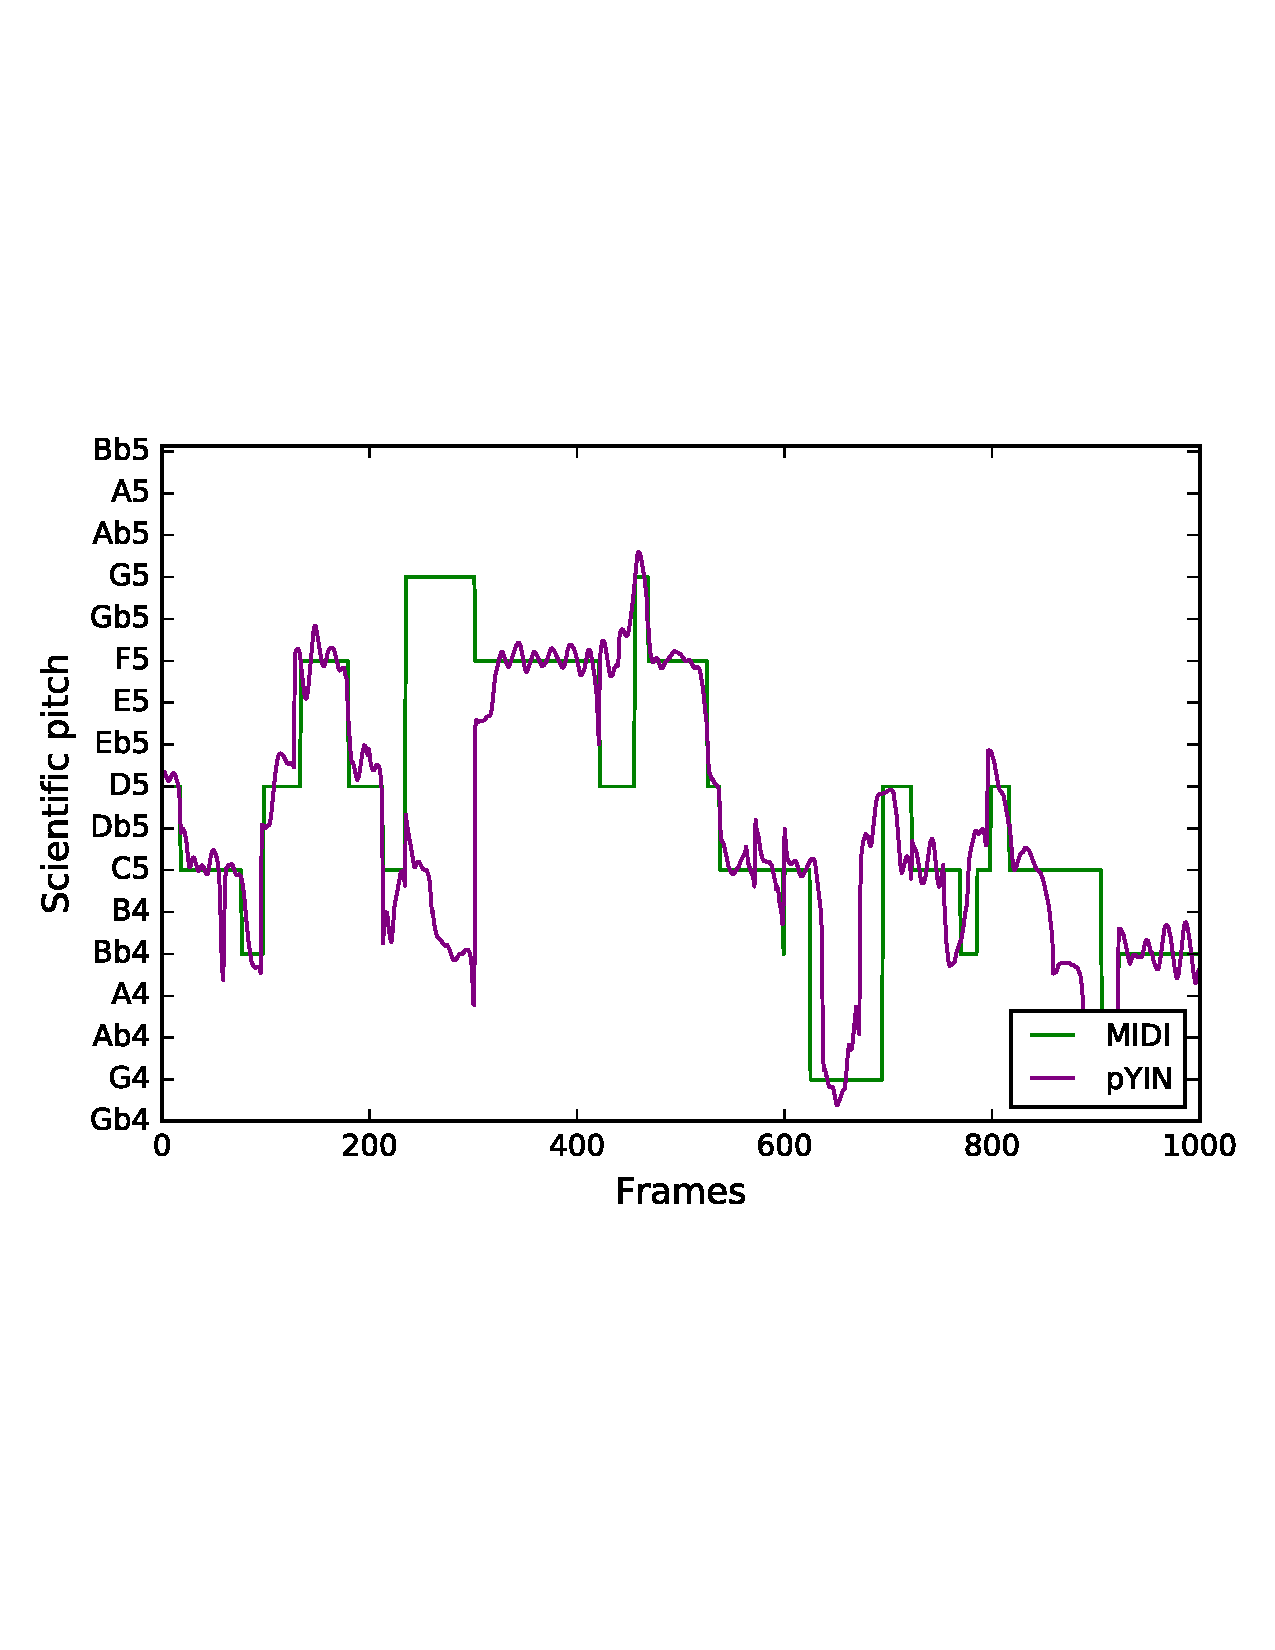
\includegraphics[width=0.5\textwidth, ]{figures/clustering_midi_and_pyin_aligned_active_545284262_2000375574.pdf}}\vspace{-0.5in}
    \subfigure{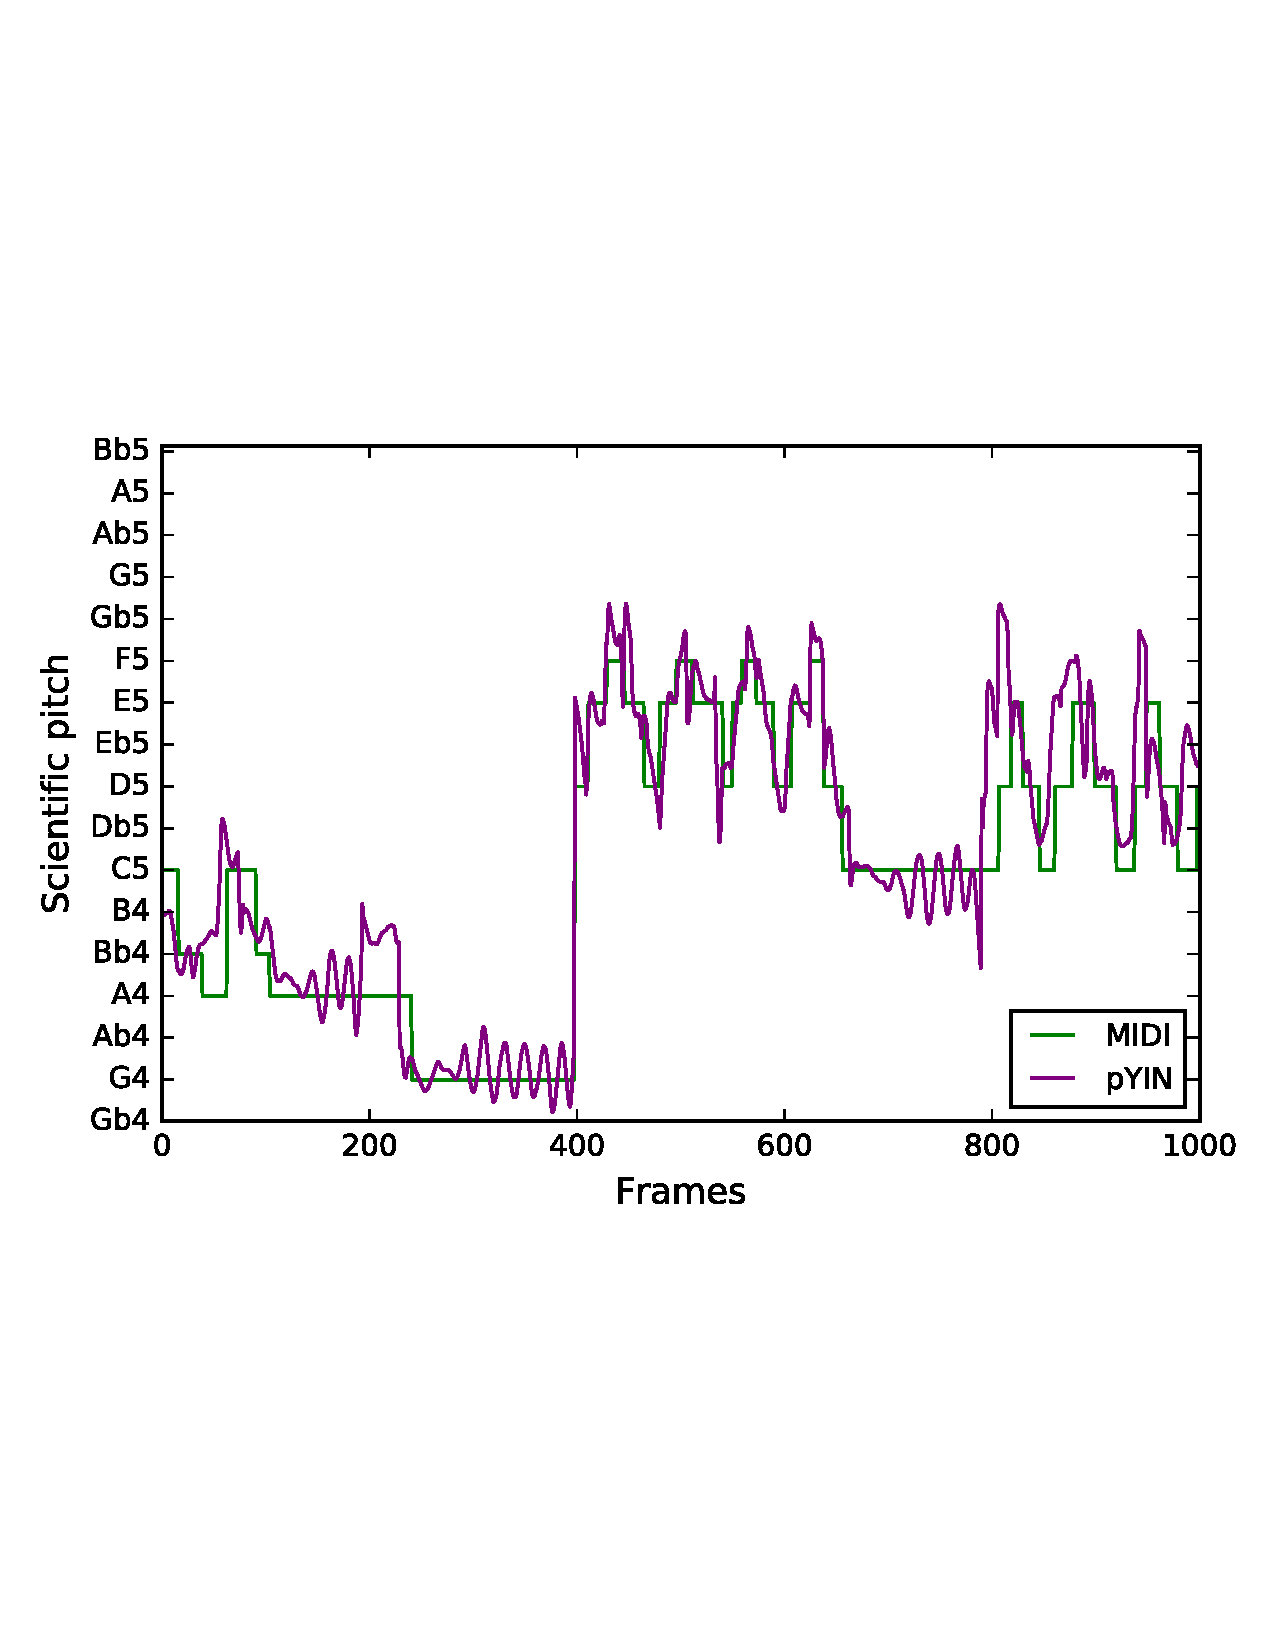
\includegraphics[width=0.5\textwidth, ]{figures/clustering_midi_and_pyin_aligned_active_54195986_1647186097.pdf}}\vspace{-0.5in}
    \caption{Singing pitch analysis of sample performances with aligned MIDI. Two are in the clusters selected for  ``Intonation'' dataset (top), two in the remaining clusters (bottom). Much can be learned about the individual performances. The top two appear more tightly aligned to the expected pitch, though the second plot contains harmonization at a major third below the musical score. The vibrato in the first plot is particularly smooth, a sign of an advanced singer. The third plot shows frequent deviation from the score, while the fourth shows deviation at the beginning and the end but accuracy in the middle, along with a smooth vibrato. Still, it is difficult visually determine from this data format whether a performance sounds ``in tune''.}
    \label{fig:sample_intonation}
\end{figure*}

%Related work
%- pitch deviation analysis
\section{Related work}
\label{sec:related}

\begin{figure}[h!]
    \centering
    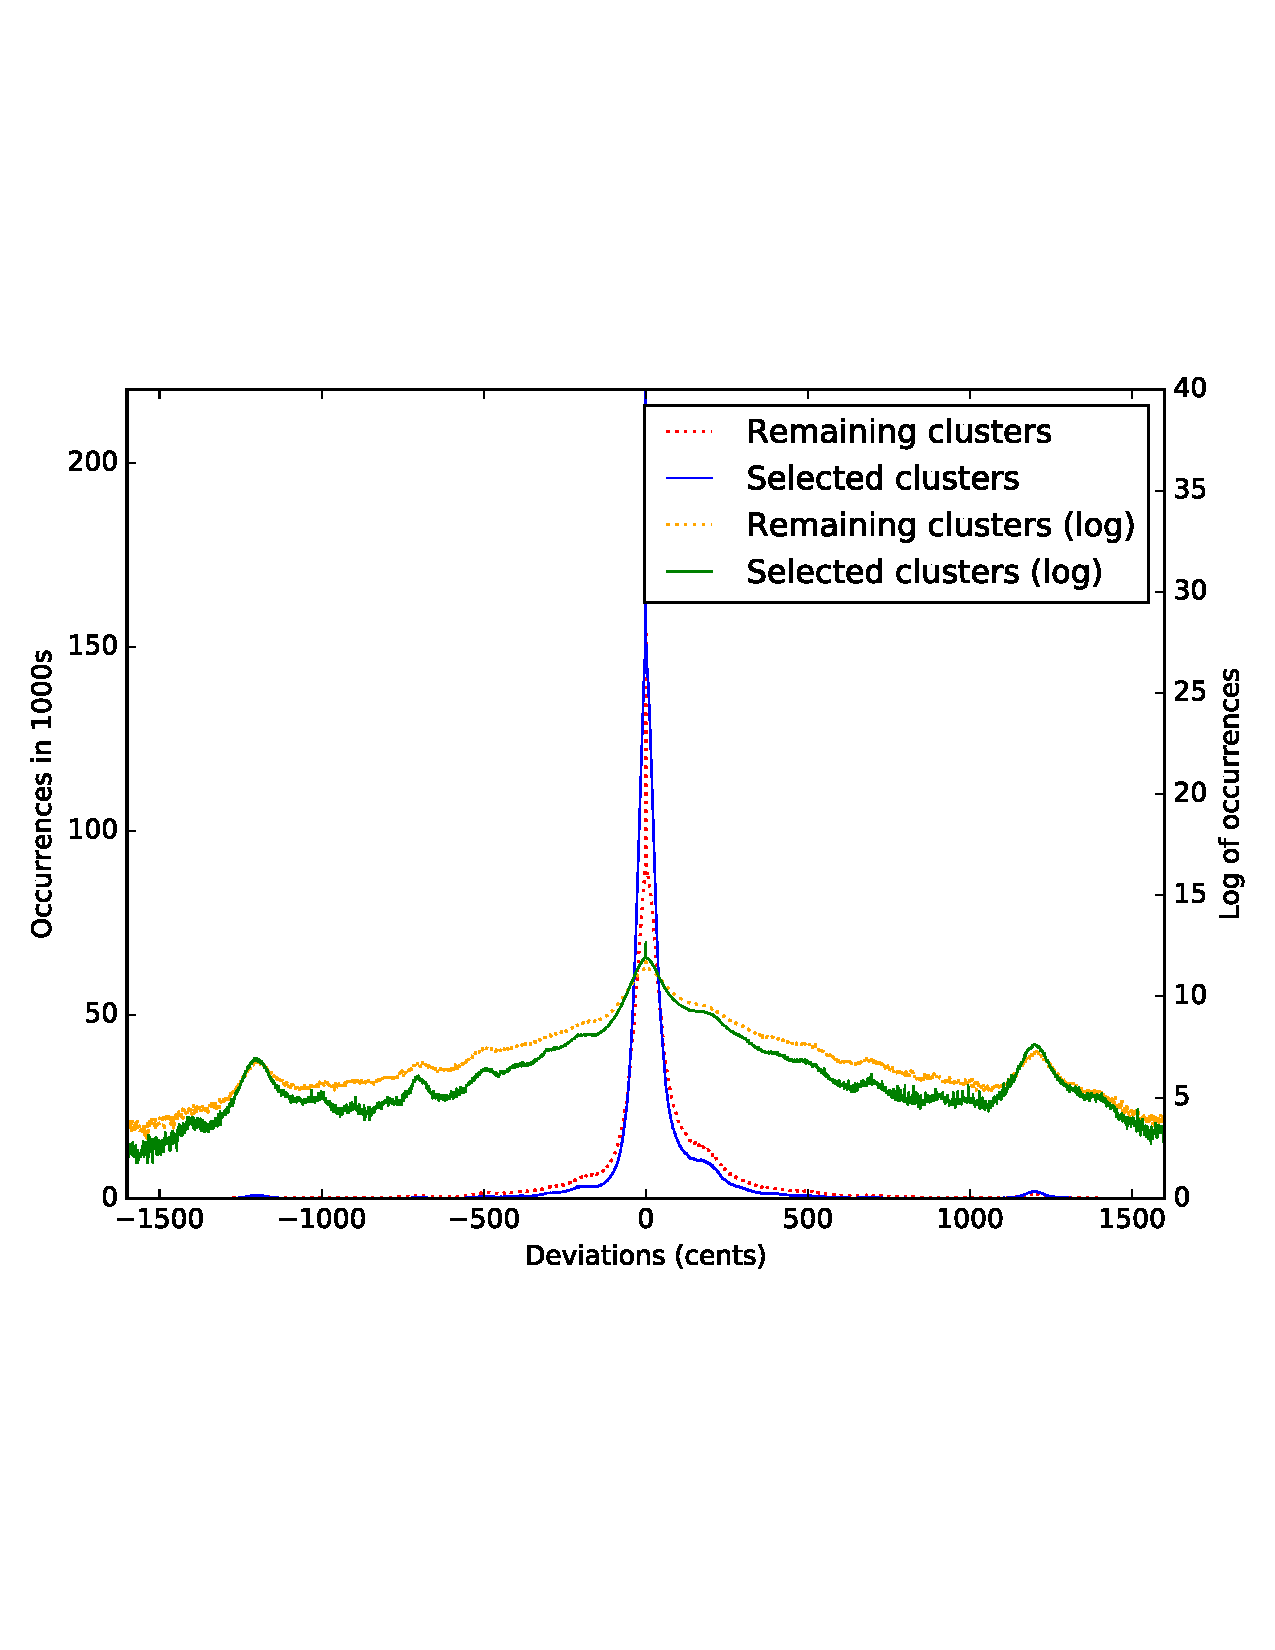
\includegraphics[width=0.75\textwidth]{figures/full_histograms_comparison.pdf}\vspace{-1in}
    \caption{Global histograms of singing pitch deviations from the expected MIDI pitch in cents summed over 4702 performances in the ``Intonation'' dataset and 4702 in the remaining clusters. The plot is truncated at the top for readability. Scaled log histograms make more noticeable the small peaks at 1200 cents in both directions, due to octave deviations, common among singers. There is also, interestingly, a larger number of deviations between 100 and 300 cents in the positive direction than in the negative direction.}
    \label{fig:full_hist}
\end{figure}

\subsection{Pitch deviation analysis}
Automatic analysis of musical intonation behavior has also been performed in other contexts. For example, the authors of \cite{nichols2012automatically} described an approach to discovering talented singers on YouTube based on features extracted mostly from the audio. One of the main features they chose consisted of a pitch deviation histogram, which characterizes intonation behavior of a full performance in a low dimension. Given that the performances were typically not associated with a musical score and that the singing was mixed with the accompaniment and other background sounds, the authors built the histogram from the Short-Time Fourier Transform amplitude peaks. A singer who sings flat should have a histogram skewed to the left, and an active vibrato will cause values to spread. Our feature extraction task is different from \cite{nichols2012automatically} because, as we describe below, we have access to the musical scores of the vocals and because the audio sources are separated. We can, therefore, apply a standard pitch detection algorithm to each vocal track and compare the results to the musical score. Comparison of performance pitch and musical score is also used by \cite{lim2010intune} in the context of a tool for musical performance visualization.


\begin{figure}[h!]
    \centering
    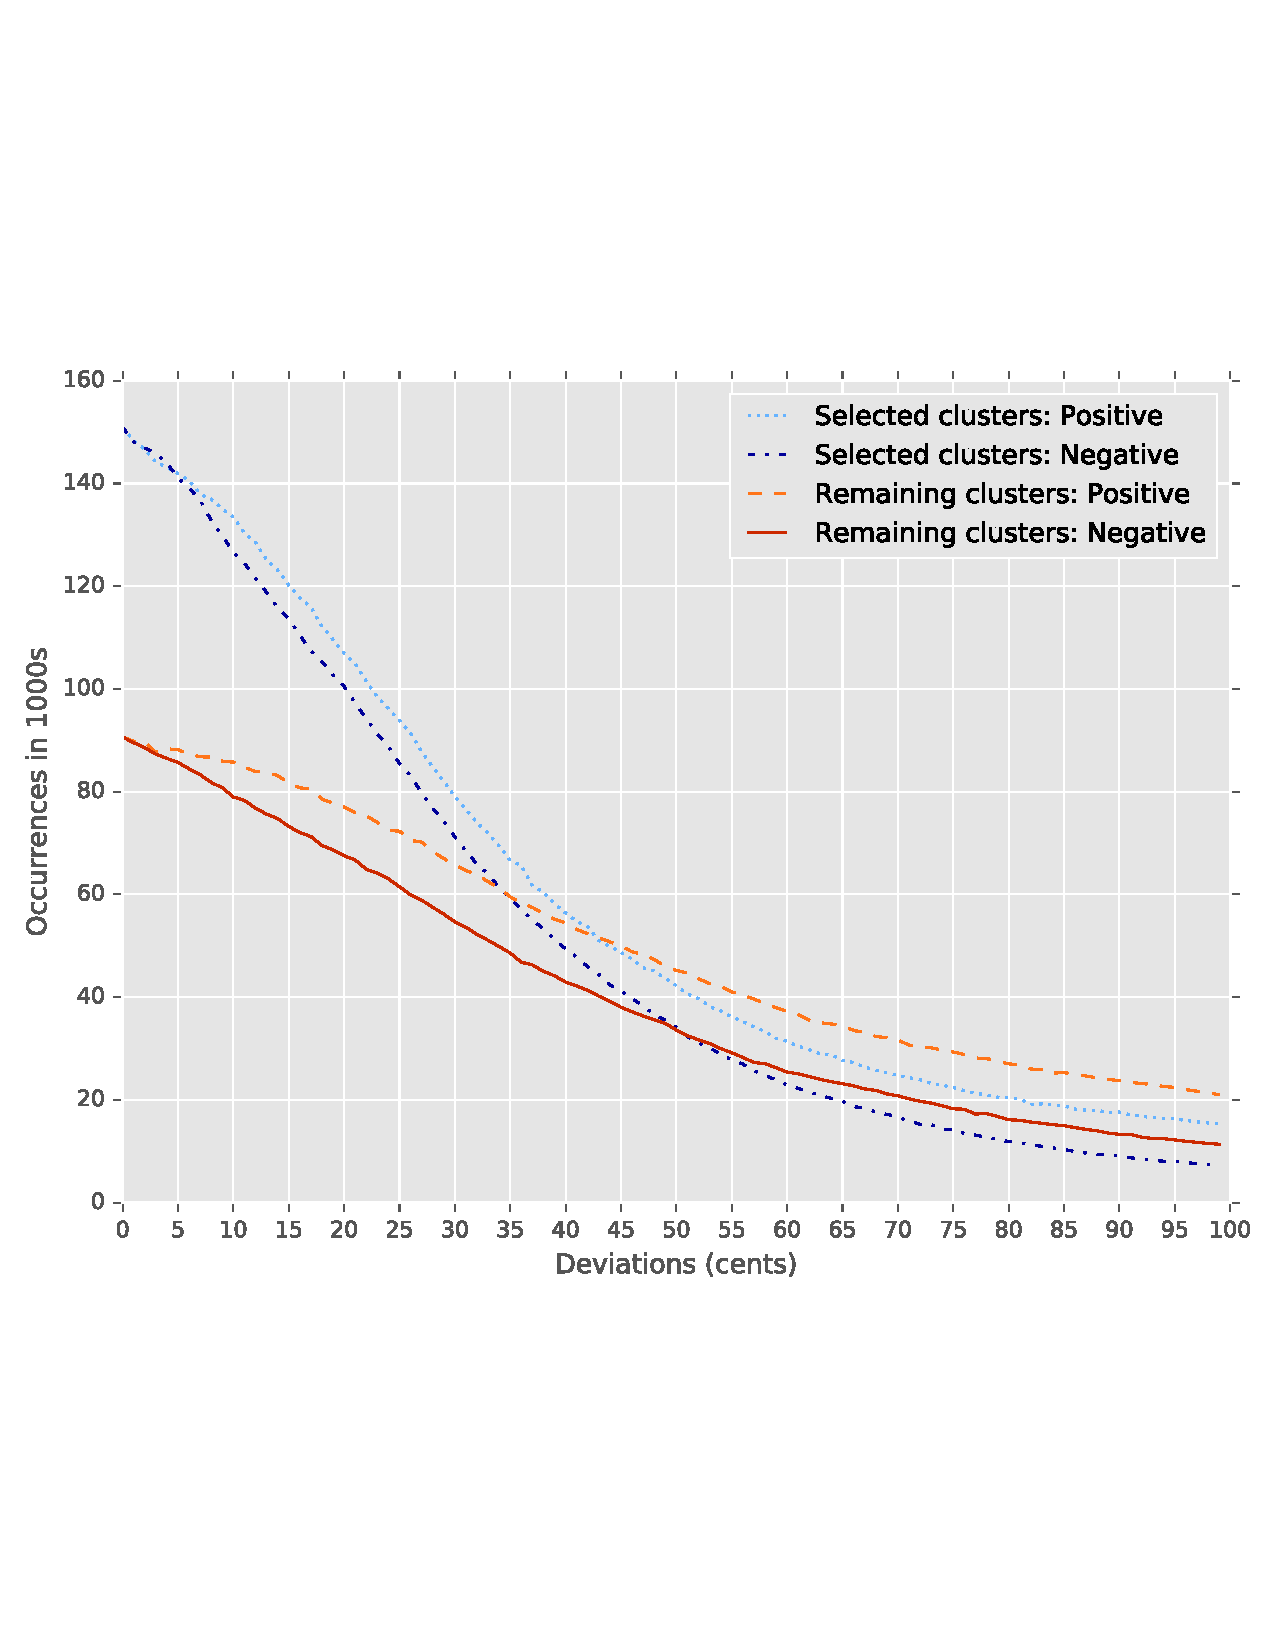
\includegraphics[width=0.75\textwidth]{figures/full_pos_vs_neg_line.pdf}\vspace{-1in}
    \caption{Comparison of positive and negative deviation counts for cents ranging from 1 to 100 (omitting 0) for both datasets. In both groups, positive deviations are more common than negative ones. The ``Intonation'' dataset deviations are more concentrated around zero. }
    \label{fig:pos_neg}
\end{figure}

%Data collection and feature extraction
\section{Data collection and feature extraction}
\label{sec:features}
We collected solo vocal tracks of karaoke performances from a very large database. The first step was to filter for performances where singers used a headset---avoiding incorporating noise from the backing track into the recording. Given that we had access to a musical MIDI score of expected pitches, we also used a simple heuristic to filter for performances that were aligned enough with the score to exclude scenarios such as people speaking instead of singing. We kept this heuristic lenient enough that in-tune performances where the singer used harmonization (sang different pitches than the expected melody) or made other intentional deviations from the MIDI track wouldn't be excluded. This pre-filtering provided 14403 performances. 

The next step was to summarize intonation patterns of a performance using a low-dimensional set of features. The procedure is shown in Figure \ref{fig:pipeline} for two example performances. We first compared the singing pitch to the expected pitch in the MIDI score. We computed the singing pitch using the pYIN algorithm \cite{mauch2014pyin} on one minute of audio, starting at 30 seconds to avoid silence, with one sample (frame) per 11 milliseconds. pYIN has a high frequency resolution because it is based in the time domain and refines results using linear interpolation. Resolution is crucial for musical intonation, where a few cents difference can determine whether a pitch sounds in or out of tune. We shifted the MIDI score by a global constant to the octave nearest to the singing pitch, which can differ based on gender, age, and vocal type. We then computed the frame-wise absolute values of the difference in cents $\left| 1200 * log_2 \frac{f_1 + \epsilon} {f_2 + \epsilon} \right|$ between the performance and MIDI score. Of this set of values, we kept the differences less than or equal to 200 cents, equivalent to two semitones, in order to focus the analysis on intonation behavior when the singer was close to the expected pitch. Larger differences could be due to many reasons, ranging from misalignment of notes in time to harmonization, and might add undesired noise to the distributions. 

Finally, we summarized these variable-length sequences of frame-wise differences in a fixed, low-dimensional representation. We generated a random sample of 10,000 differences with replacement for every performance and kept 31 evenly spaced quantiles. This empirically chosen number is large enough to effectively summarize the characteristics of the distribution but produces a low enough dimensionality for clustering.

\begin{figure}[h!]
    \centering
    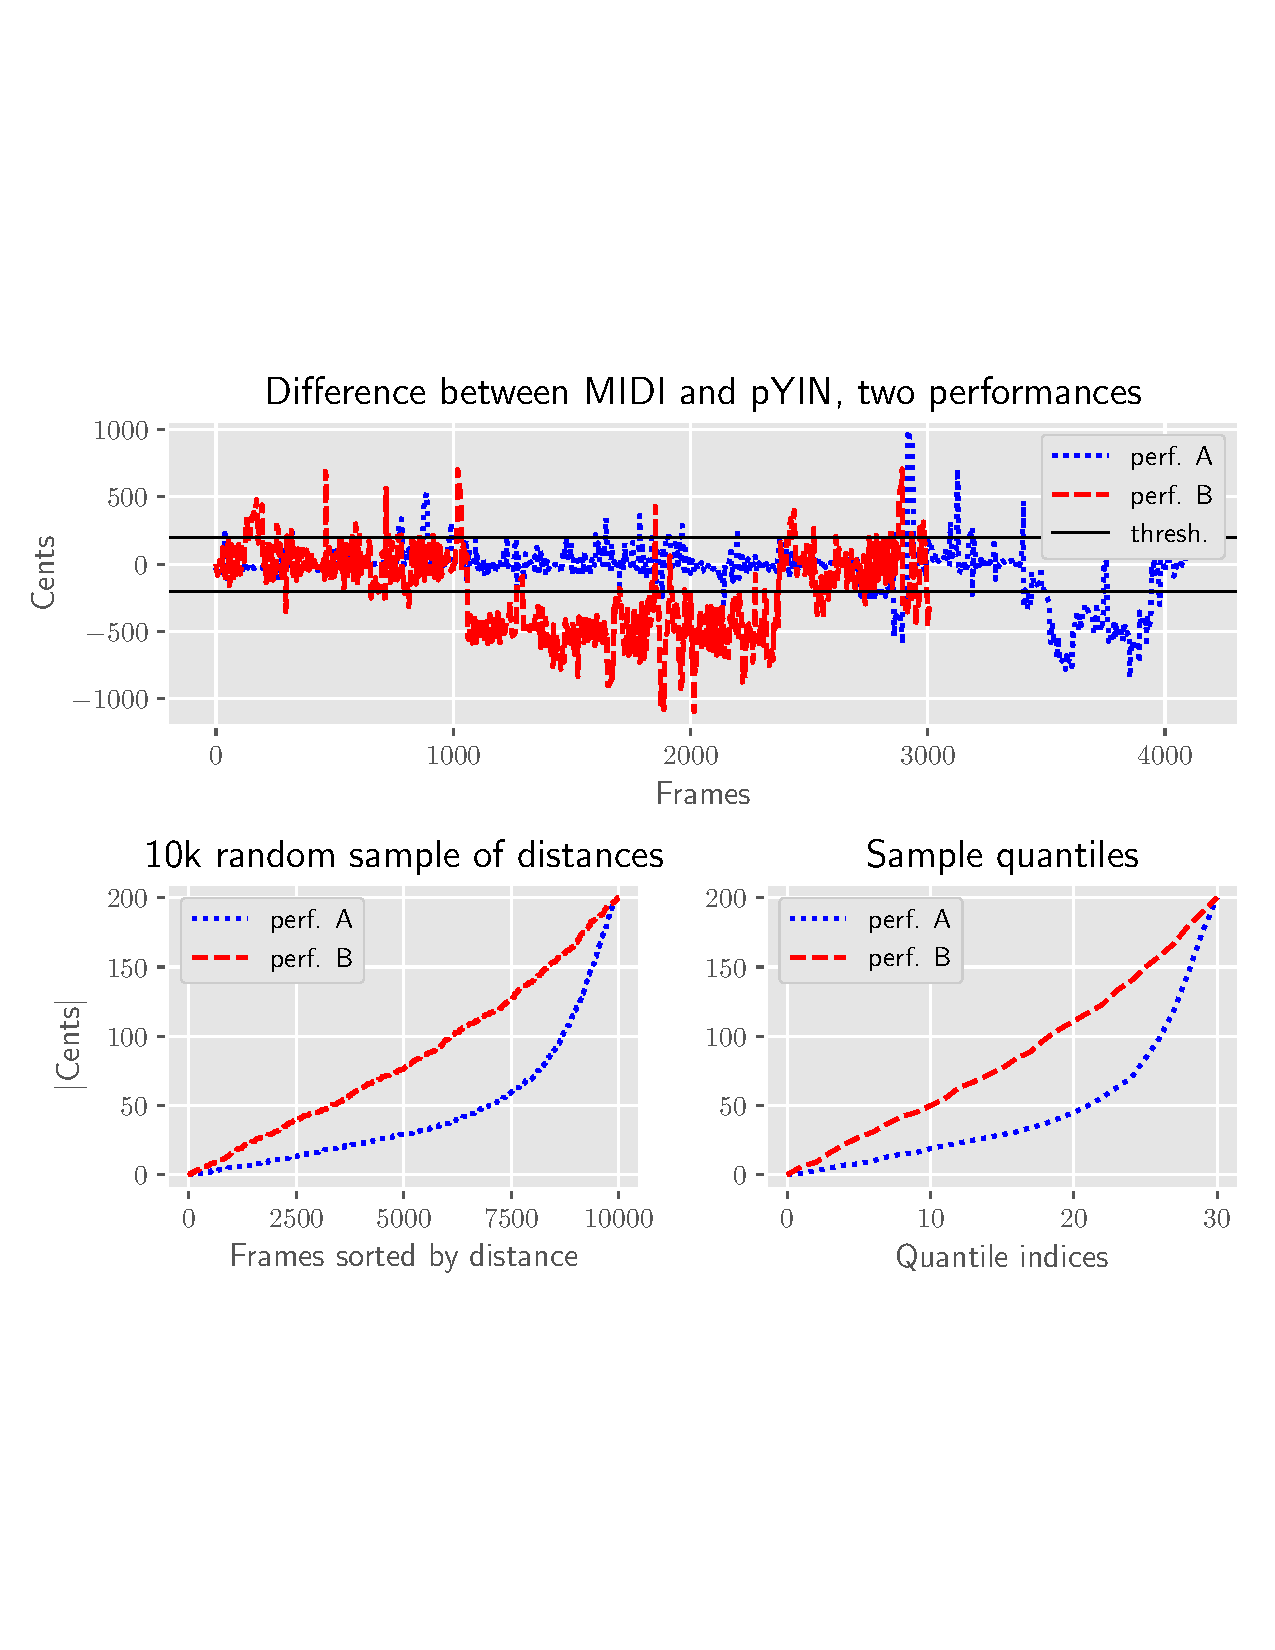
\includegraphics[width=0.75\textwidth]{figures/data_processing_pipeline.pdf}\vspace{-1in}
    \caption{Data pre-processing steps for two example performances. The blue performance was selected for the ``Intonation'' dataset and the red performance was not. The first plot shows the frame-wise differences in cents between the measured singing pitch and equal-tempered MIDI score. We computed the absolute values of these differences and discarded those whose deviation was larger than 200 cents. The second plot shows random samples of 10,000 from the frame-wise difference lists, sorted by distance. The blue curve shows less deviation from the expected pitch than the red. The third plot shows 31 quantiles summarizing the curve in the second plot in a lower dimension.}
    \label{fig:pipeline}
\end{figure}
%Spectral clustering
\section{Spectral clustering}
As suggested by the studies described in Section \ref{sec:intonation}, an advanced singer might produce wider pitch deviations, due to a pronounced vibrato or expressive variations such as pitch bending, time shifting, or harmonization, than a singer who sings close to the musical score but is slightly off pitch. For this reason, we didn't try to select performances based on a simple metric like average distance of singing pitch from the score. We also didn't attempt to directly model ``being in tune'', instead adopting a semi-supervised approach that clusters performances based on features generated from the deviations. We then chose which cluster to keep by listening to samples from each.

We applied spectral clustering to the summarized performances using the signless Laplacian matrix as the adjacency graph \cite{lucinska2012spectral}. This graph is based on selecting nearest neighbors (50 in our case). In practice, we clustered approximately 5000 songs at a time into 3 or 4 clusters, depending on which value produced better Newman modularity \cite{newman2006modularity}. We then listened to 50 samples from every cluster and subjectively determined the intonation of every performance by evaluating it as ``in tune'', ``neutral'', ``out of tune''. Consistently, one cluster produced distinctly good results with roughly 75 per cent of the songs classified as ``in tune'' and many of the remaining songs being classified as ``neutral'' rather than ``out of tune'', while the other clusters had only a small percentage of performances classified as ``in tune''. 

Keeping the samples from the selected clusters resulted in the ``Intonation'' dataset of 4703 performances. Though not every performance is in tune and not every performance in remaining clusters is out of tune, a majority of in-tune performances in this dataset suffices for many machine-learning applications.

%Analysis
\section{Analysis}

The quality of the dataset is difficult to measure without a subjective listening test. At this point, we do not attempt to directly show that the ``Intonation'' dataset performances have better intonation than those in the remaining clusters. Instead, we show a difference in the intonation behavior distributions in the two collections. In order to compare samples of the same size, we analyzed the full ``Intonation'' dataset of size 4702 and a randomly selected a sample of the same size of performances from the remaining clusters.

\subsection{Data pre-processing for analysis}
We computed the frame-wise differences between singing pitch and MIDI score similarly to the way described in Section \ref{sec:features}. Unlike before, we retained the sign instead of taking the absolute value in order to know whether the pitch was sharp or flat. We also kept all deviations instead of discarding those larger than 200 cents: At the analysis stage, we are interested in intonation characteristics across the whole performance, including the larger deviations due to harmonization, expressive deviations, or inaccuracy. 

To minimize misalignment before computing the deviations, we applied Dynamic Time Warping (DTW) \cite{berndt1994using} to better align the MIDI and singing pitch tracks. This algorithm stretches both signals in time in a way that minimizes the total sum of distances between the two. We used the algorithm as described in \cite{muller2015fundamentals} and implemented in \cite{mcfee2015librosa}. To avoid distorting the pitch track, we forced the algorithm to apply most time warping to the MIDI, which consists of straight lines. We discarded frames where either the musical score or pitch tracks were silent in order to only consider active frames in our analysis. Figure \ref{fig:sample_intonation} shows four example performances after the initial processing. The top two are from the selected clusters and the bottom two from the remaining clusters.

\subsection{Pitch deviation histogram}
We compared the sequences of frame-wise pitch deviations from the selected clusters to those from the remaining clusters. Similarly to \cite{nichols2012automatically}, we computed histograms of the deviations from the equal-tempered MIDI score summed over all performances in each group, normalizing them to have the same total counts. Figure \ref{fig:full_hist} shows that the ``Intonation'' dataset deviations are more concentrated very close to 0 than those in the remaining clusters. The same can be observed at other harmonization peaks, $\pm1200$ cents (an octave) and other values in between, indicating more intentional harmonization and less accidental deviation. There is also, interestingly, a higher concentration of counts between 100 and 300 cents especially in the positive direction, maybe due to harmonization and expressive suspensions.

\subsection{Pitch deviation probabilities}
We examined whether we could find intonation tendencies like those described in Section \ref{sec:intonation}. Unlike in the data used in the cited studies, the backing tracks are fixed recordings, so all pitch adjustments happen in the voice. This can affect the pitch deviation distributions. In Figure \ref{fig:pos_neg}, we examine deviations within 100 cents because a larger deviation corresponds a different note. Both collections tend towards positive deviations, but the tail is lighter in the selected clusters.

We quantify this result by estimating the probability of positive versus negative deviations within various absolute deviation thresholds using bootstrapping \cite{efron1994introduction} with 10000 iterations, as shown in Table \ref{table:1}. We choose ranges of cents that are of interest when comparing theoretical musical intervals generated using the equal temperament versus other intonation systems (e.g., Pythagorean or Just intonation, described in the cited studies). Use of other intonation systems would explain deviations of 2 to 16 cents. We first examine the ratio of deviations less than 2 cents. As expected, a probability of 0.5 shows no significant preference for sharp versus flat intonation. Within 2 to 16 cents, we get 0.51. However, the largest probabilities occur at larger values, 300 cents. We cannot determine whether this deviation is a desirable effect or due to an unknown factor. The tendencies are observed in both collections. 


\begin{table}[t!]
\centering
\begin{tabular}{ |c|c|c| } 
\hline
\multicolumn{3}{|c|}{Results from ``Intonation'' dataset (4702 performances)}\\
\hline\hline
Cents range & Negative/positive deviation ratio & Var \\
\hline
1 to 2 & 0.500 & 0.001 \\ 
2 to 16 & 0.506 & 0.001 \\ 
1 to 100 & 0.532 & 0.002\\ 
100 to 300 & 0.727 & 0.002\\ 
\hline\hline
\multicolumn{3}{|c|}{Results from other performances (9701 performances)}\\
\hline\hline
Cents range & Negative/positive deviation ratio & Var \\
\hline
1 to 2 & 0.500 & 0.001 \\ 
2 to 16 & 0.509 & 0.001 \\ 
1 to 100 & 0.541 & 0.002\\ 
100 to 300 & 0.700 & 0.002\\ 
\hline
\end{tabular}
\caption{Probability estimates of positive versus negative frame-wise deviations of singing pitch from the equal-tempered MIDI score, computed using bootstrapping. The analysis was performed within different ranges of interest. When the deviation is less than 100 cents, the singer did not sing a different note. We found a particularly strong tendency towards positive deviations in the range of 100 to 300 cents.}
\label{table:1}
\end{table}

%Dataset description and applications
\section{Dataset description and applications}
The ``Intonation'' dataset contains the full unmixed and unprocessed vocal tracks of 4702 performances. It consists of 474 unique arrangements by 3556 singers. It also contains the pYIN pitch analysis and multiple backing track features for the range of 30 to 90 seconds: constant-Q transform, chroma, mel-frequency cepstrum coefficients, root mean square error, and onset, all computed using the Librosa \cite{mcfee2015librosa} package. Metadata of the performances is included. The dataset has applications ranging from the study of singing style in the context of karaoke performances, with optional study of user meta-data, to machine learning. For example, the vocal tracks can be used for informed source separation, an approach similar to separation by humming, described in \cite{smaragdis2009separation} and \cite{liutkus2012informed}. Similarly, the dataset can be used for training a query-by-humming system, in a similar way to \cite{huq2010crowdsourcing}. The vocal pitch tracks and backing track features can be used to study autotuning applications trained on real-world singing and develop a proof-of-concept model for vocal pitch correction \cite{wager2018pitch}.

%Conclusion
\section{Conclusion}
We present a semi-automatic process for the task of searching through a large database of amateur karaoke performances for samples with a tendency for good musical intonation. The approach can be applied in other situations where a researcher needs to extract a subset of data samples from a large database. We show that the set of collected performances has a different intonation behavior distribution than the set of remaining performances. The resulting public dataset, ``Intonation'', of 4702 performances is available on the Stanford CCRMA DAMP website. The ``Intonation'' dataset can be used for music information retrieval applications like query-by-humming systems. Analyzing the dataset, we find that pitch deviations between the measured singing pitch and the MIDI score are more often positive than negative, implying that singers more often choose higher frequencies.

\end{appendices}

%%%%%%%%%%%%%%%%
% References
%%%%%%%%%%%%%%%%
%\begin{singlespace}  % use single-line spacing for multi-line text within a single reference
%	\setlength\bibitemsep{\baselineskip}  %manually set separataion betwen items in bibliography to double space
%	\printbibliography[heading=bibintoc,title={References}]
%\end{singlespace}
\printbibliography[heading=bibintoc,title={References}]
%\addcontentsline{toc}{chapter}{References}  %add References section to Table of Contents

%%%%%%%%%%%%%%%%
% Vita 
% Only for PhD students
% Masters students remove this line
%%%%%%%%%%%%%%%%
\chapter*{Curriculum Vitae}
\addtocontents{toc}{
 \unexpanded{\unexpanded{\renewcommand{\cftchapdotsep}{\cftnodots}}}%  
}
\addcontentsline{toc}{chapter}{Curriculum Vitae}

%%%%%%%%%%
%-----CUSTOM COMMANDS FOR FORMATTING SECTIONS----------------------------------
\newcommand{\CVItem}[1]{
  \item\small{
    {#1 \vspace{-2pt}}
  }
}

\newcommand{\CVSubheading}[4]{
  \vspace{-2pt}\item
    \begin{tabular*}{0.97\textwidth}[t]{l@{\extracolsep{\fill}}r}
      \textbf{#1} & #2 \\
      \small#3 & \small #4 \\
    \end{tabular*}\vspace{-7pt}
}

\newcommand{\CVSubSubheading}[2]{
    \item
    \begin{tabular*}{0.97\textwidth}{l@{\extracolsep{\fill}}r}
      \text{\small#1} & \text{\small #2} \\
    \end{tabular*}\vspace{-7pt}
}

\newcommand{\CVSubItem}[1]{\CVItem{#1}\vspace{-4pt}}

\renewcommand\labelitemii{$\vcenter{\hbox{\tiny$\bullet$}}$}

\newcommand{\CVSubHeadingListStart}{\begin{itemize}[leftmargin=0.5cm, label={}]}
% \newcommand{\resumeSubHeadingListStart}{\begin{itemize}[leftmargin=0.15in, label={}]} % Uncomment for US
\newcommand{\CVSubHeadingListEnd}{\end{itemize}}
\newcommand{\CVItemListStart}{\begin{itemize}}
\newcommand{\CVItemListEnd}{\end{itemize}\vspace{-5pt}}
%%%%%%%%%%

%-----EDUCATION----------------------------------------------------------------
\vspace{-30pt}
\singlespacing
\section*{EDUCATION}
%\vspace{-8pt}
  \CVSubHeadingListStart
%    \CVSubheading % Example
%      {Degree Achieved}{Years of Study}
%      {Institution of Study}{Where it is located}
    \CVSubheading
      {{Doctor of Philosophy in Informatics $|$ \emph{\small{Music Track}}}}{Aug. 2014 -- Feb. 2021}
      {Indiana University Bloomington}{Bloomington, Indiana, USA}
    \CVSubheading
      {Master of Science in Computer Science}{Aug. 2014 -- May 2018}
      {Indiana University Bloomington}{Bloomington, Indiana, USA}
    \CVSubheading
      {{Bachelor of Music $|$ \emph{\small{Major: Bassoon, Minor: Mathematics}}}}{Aug. 2009 -- May 2014}
      {Indiana University Bloomington}{Bloomington, Indiana, USA}
  \CVSubHeadingListEnd

%-----WORK EXPERIENCE----------------------------------------------------------

\section*{WORK EXPERIENCE}
%\vspace{-8pt}
  \CVSubHeadingListStart
  
    \CVSubheading
      {Research Scientist Intern, Music Intelligence Group}{Fall 2019 -- Winter 2020}
      {Spotify S.A.}{New York City, NY}
    \CVSubheading
      {Applied Scientist Intern, Alexa Speech}{Summer 2019}
      {Amazon, Inc.}{Santa Clara, CA}
    \CVSubheading
      {Audio Engineering Intern}{Summer 2018}
      {Smule, Inc.}{San Francisco, CA}
    \CVSubheading
      {Software Engineering Intern, Android Audio}{Summer 2017}
      {Google, Inc.}{Mountain View, CA}
    \CVSubheading
      {Teaching Assistant, Informatics and Computing}{Fall 2014 -- Spring 2016}
      {Indiana University Bloomington}{Bloomington, Indiana, USA}
    %\CVItemListStart
    %\CVItem{INFO-I547: Music Information Processing: Audio }
    %\CVItem{CSCI-B555: Machine Learning }
    %\CVItem{INFO-I101:Introduction to Informatics}
    %\CVItem{INFO-I201: Mathematical Foundations for Informatics}
    %\CVItemListEnd
  \CVSubHeadingListEnd


%-----CONFERENCES AND PRESENTATIONS--------------------------------------------

\section*{PUBLICATIONS AND PRESENTATIONS}

\hspace{\parindent}\textbf{S. Wager, G. Tzanetakis, C. Wang, and M. Kim}. ``Deep Autotuner: A Pitch Correcting Network for Singing Performance''. in Proc. IEEE Int. Conf. Acoustics, Speech, and Signal Processing (ICASSP), 2020.

\textbf{S. Wager, A. Khare, M. Wu, and S. Sundaram}. ``Fully learnable front-end for multi-channel acoustic modeling using semi-supervised learning,'' in Proc. IEEE Int. Conf. Acoustics, Speech, and Signal Processing (ICASSP), 2020.

\textbf{S. Wager, G. Tzanetakis, S. Sullivan, C. Wang, J. Shimmin, M. Kim, and P. Cook}. ``Intonation: a dataset of quality vocal performances refined by spectral clustering on pitch congruence,'' in Proc. IEEE Int. Conf. Acoustics, Speech, and Signal Processing (ICASSP), 2019.

\textbf{S. Wager and M. Kim}. ``Collaborative speech dereverberation: regularized tensor factorization for crowdsourced multi-channel recordings,'' in Proc. IEEE European Signal Processing Conf. (EUSIPCO), 2018.

\textbf{S. Wager, L. Chen, M. Kim, and C. Raphael}. ``Towards expressive instrument synthesis through smooth frame-by-frame reconstruction: From string to woodwind,'' in Proc. IEEE Int. Conf. Acoustics, Speech and Signal Processing (ICASSP), 2017.




\pagenumbering{gobble}

\end{document}
